\documentclass[12pt,a4paper]{book}
\usepackage[utf8]{inputenc}
\usepackage[spanish]{babel}

% Paquetes

\usepackage{amsmath}
\usepackage{amsfonts}
\usepackage{amssymb}
\usepackage{amsthm}  % Permite crear teoremas nuevos / Estilos de teoremas 
\usepackage{graphicx} % 
\usepackage[colorlinks=true,allcolors=blue]{hyperref} % Crea las hiperreferencias (clicas y te mueves)
\graphicspath{ {Imagenes/} }
\usepackage{fancybox} % para usar la caja de los ejemplos
\usepackage{subcaption}

% Autor y titulo

\title{Apuntes Óptica II}
\author{Daniel Vázquez Lago}

% Forma del  texto

\setlength{\parindent}{15px}
\usepackage[left=2.25cm,right=2cm,top=4cm,bottom=2cm]{geometry}

% Otros

\numberwithin{equation}{section}
\numberwithin{figure}{section}

% Comandos propios
\newcommand{\tquad}{\quad \quad \quad}

\newcommand{\parentesis}[1]{\left( #1  \right)}
\newcommand{\parciales}[2]{\frac{\partial #1}{\partial #2}}
\newcommand{\pparciales}[2]{\parentesis{\parciales{#1}{#2}}}
\newcommand{\ccorchetes}[1]{\left[ #1  \right]}
\newcommand{\D}{\mathrm{d}}
\newcommand{\derivadas}[2]{\frac{\D #1}{\D #2}}
\newcommand{\cte}{\mathrm{cte}}

\newcommand{\estado}[1]{| \Psi_{ #1} \rangle}
\newcommand{\1}{_{(1)}}
\newcommand{\2}{_{(2)}}
\newcommand{\Real}{\mathrm{Re} }
\newcommand{\sinc}{\mathrm{senc} }

\newcommand{\intinf}{\int_{-\infty}^{\infty}}

\newcommand{\TF}{\mathrm{TF}}

% Comandos vectoriales

\newcommand{\xn}{\mathbf{x}}
\newcommand{\yn}{\mathbf{y}}
\newcommand{\zn}{\mathbf{z}}
\newcommand{\vn}{\mathbf{v}}
\newcommand{\un}{\mathbf{u}}
\newcommand{\rn}{\mathbf{r}}
\newcommand{\qn}{\mathbf{q}}
\newcommand{\pn}{\mathbf{p}}
\newcommand{\kn}{\mathbf{k}}
\newcommand{\sn}{\mathbf{s}}
\newcommand{\an}{\mathbf{a}}
\newcommand{\bn}{\mathbf{b}}
\newcommand{\nn}{\mathbf{n}}


\newcommand{\rhon}{\mathbf{\rho}}


\newcommand{\An}{\mathbf{A}}
\newcommand{\Pn}{\mathbf{P}}
\newcommand{\Sn}{\mathbf{S}}
\newcommand{\En}{\mathbf{E}}
\newcommand{\Hn}{\mathbf{H}}
\newcommand{\Encal}{\boldsymbol{\mathcal{E}}}
\newcommand{\Ecal}{\mathcal{E}}
\newcommand{\Esf}{\mathsf{E}}

\newcommand{\Ccal}{\mathcal{C}}
\newcommand{\Scal}{\mathcal{S}}

% Comandos vectoriales unitarios

\newcommand{\hrho}{\hat{\rhon}}
\newcommand{\hnu}{\hat{\un}}
\newcommand{\hns}{\hat{\sn}}
\newcommand{\hnr}{\hat{\rn}}
\newcommand{\hnx}{\hat{\xn}}
\newcommand{\hny}{\hat{\yn}}
\newcommand{\hnz}{\hat{\zn}}
\newcommand{\hnn}{\hat{\nn}}

% Comandos teoremas

\newtheorem{theorem}{Teorema}[section]
\newtheorem{principio}{Principio}[section]

\theoremstyle{definition}
\newtheorem{definition}{Definicion}[section]
\begin{document}

\maketitle

\newpage

\tableofcontents

\newpage
\chapter{Ondas y discontinuidades paraxiales}

\section{Fundamentos de las ondas localmente planas}
\subsection{Ondas planas}

Para entender que es una onda plana primero debemos saber que es una \textbf{onda plana}. Una onda plana armónica definida en un medio de índice de refracción $n_0$ viene dado por:

\begin{equation}
\En (\rn,t) = \Encal  e^{i (\kn \cdot \rn - \omega t)}
\end{equation}
donde $ \Encal = \mathcal{E} \hnu$, siendo $\mathcal{E}$ una constante con unidades de campo eléctrico. La notación caligráfica se usa cuando los campos (o las variables) no dependen del tiempo. Puede ser una función compleja (espacial), pero no dependerá de $e^{-i \omega t}$. Definimos como \textbf{vector número de onda} $\kn$ al vector:

\begin{equation}
\kn \equiv n_0 k_0 \hns
\end{equation}
donde $\hns$ (en las ondas planas y las ondas localmente planas) será el vector unitario de Poyting, que nos da la dirección de la propagación de energía. Al factor $k_0$ lo llamamos número de onda en el vacío. En general en un medio cualquiera $k=n_0 k_0$ es el número de onda, a partir del cual podemos calcular la \textbf{longitud de onda}:

\begin{equation}
\lambda = \dfrac{2 \pi}{k}
\end{equation}

Como podemos ver existe entonces una fase dependiente del tiempo y una fase dependiente del espacio.

\subsection{Ondas localmente planas}

 Supongamos ahora que en realidad la onda plana no es mas que la aproximación de orden cero de una serie de Taylor. En ese caso las ondas localmente planas no serán mas que las ondas que surgen al aumentar el uno el orden de la aproximación, tal que:
 
\begin{equation}
\En (\rn,t) = \Encal (\rn) e^{-i \omega t} = \mathsf{E} (\rn_0) e^{ik_0[\mathcal{L} (\rn_0) + \nabla \mathcal{L} (\rn_0) (\rn - \rn_0)]} e^{- i \omega t}
\end{equation}
Cuando hablamos de un campo sin fase temporal, lo denotamos por letras caligráficas ($\mathcal{E}$ en el caso de un campo eléctrico). Si no lleva fase espacia y temporal, denotaremos el campo eléctrico con la caligrafía $\mathsf{E}$ (puede ser compleja, ya que puede llevar fase en el vector, o una fase constante, pero no dependerá de $(\rn,t)$). Aunque lo hagamos así ahora para una mayor inteligibilidad, en muchas ocasiones por no ser pedante se asumirá que el lector entiende las diferencias. Esta será la expresión de la \textbf{onda localmente plana} (LP). Esta expresión será valida en toda región del espacio de radio medio $\bar{R} \gg \lambda_0$. Dicha condición nos permite asegurar que los términos restantes tienden a cero, y por tanto constituye una buena aproximación de la realidad.

\section{Solución Eikonal de ondas localmente planas}

\subsection{Ecuación Eikonal}

En cualquier caso, hemos introducido un parámetro $\mathcal{L} (\rn)$ dependiente de la posición, de tal forma que en la fase aparece un término constante y un término dependiente del gradiente de dicho parámetro $\mathcal{L}$. Denominamos a $\mathcal{L}$ como el \textit{camino óptico}. \\

Podemos ver un paralelismo obvio entre la la ecuación de ondas planas y la ecuación de ondas localmente planas. Aunque a diferencia de las ondas planas ahora el vector de Poyting depende de la posición, podemos ver claramente que:

\begin{equation}
\hns (\rn) = \dfrac{\nabla \mathcal{L} (\rn)}{n} \label{Ec:01.02.1-Poyting_unitario}
\end{equation}

De aquí se obtiene la \textbf{ecuación Eikonal (EIK)} la cual es una ecuación diferencial no lineal para la fase espacial de la onda, aunque su deducción es trivial. Dado que $\hns$ es unitario $\hns^2 =1$. Consecuentemente:

\begin{equation}
(\nabla \mathcal{L})^2 = n^2
\end{equation}

\subsection{Vector de Poyting}

El \textbf{vector de Poyting} $\langle \Sn \rangle$ (no unitario) viene dado el promedio del producto vectorial de $\En$ y $\Hn$, tal que:

\begin{equation}
\langle \Sn \rangle  = \langle \En \wedge \Hn \rangle
\end{equation}
Dado que las ondas armónicas verifican que $\langle \En \wedge \Hn \rangle = \frac{1}{2} \En \wedge \Hn^*$. Teniendo esto en cuenta, según la ecuaciones de Maxwell se verifica que

$$ \Hn = \dfrac{1}{c \mu_0} (\hns \wedge \En^* ) $$
En ese caso podremos expresar el vector de Poyting como:

\begin{equation}
\langle \Sn \rangle \equiv \dfrac{n}{2 c \mu_0} \mathcal{E}^2 (\rn) \hns  (\rn)
\end{equation}
Aunque solo sea por consistencia, introduciremos la \textbf{teorema de Poyting}, que no es mas que la ecuación de continuidad para la energía en el campo electromagnético. Este nos dice que la variación temporal de la energía (energía mecánica y energía acumulada en los campos electromagnéticos)en un volumen es igual al flujo de energía que llega a través de dicha superficie. Escrito de manera diferencial, siendo $u_{mec}$ la energía mecánica por unidad de volumen:

\begin{equation}
\parciales{ \parentesis{u_{mec} + u_{em}}}{t} = \nabla \Sn \label{Ec:01.01.4-Th-Poyting}
\end{equation} 


\subsection{Amplitud de las ondas localente planas}

Aunque pueda parecer raro (ya que hasta ahora hemos trabajado con onda planas), la amplitud puede depender de la posición estudiada. Como sabemos la irradiancia depende del cuadrado del campo eléctrico. La conservación de la energía es vital a la hora de estudiar la irradiancia, y por tanto también a la hora de estudiar la amplitud del campo eléctrico. La conservación local de la energía en virtud del \ref{Ec:01.01.4-Th-Poyting} nos exige que $\langle \nabla \Sn \rangle$ sea cero. De esta manera tenemos que:

$$ \nabla (\mathcal{E}^2 (\rn ) \cdot \nabla \mathcal{L}) = 0 $$
De lo que se puede obtener (sin hacer un gran esfuerzo) que:

\begin{equation}
 \mathcal{E} (\rn) = A_0 \exp \ccorchetes{ - \int_{\rn_0}^{\rn} \frac{\nabla^2 \mathcal{L}}{2 n^2}  \nabla \mathcal{L} \cdot \D \rn }  = A_0 \mathcal{F} (\rn)
\end{equation}
siendo $\rn_0$ el punto de origen de la radiación electromagnética. Obviamente el término $\mathcal{F}(\rn)$ indica la \textit{fase espacial} que posee el campo eléctrico.
\subsection{Solución Eikonal}

Una vez hemos deducido cual es la forma de la fase espacial para la ecuación de ondas, y cual debe ser la forma de la amplitud para asegurar la conservación de energía, tenemos todos los ingredientes para formular la \textbf{solución Eikonal} del campo eléctrico:

\begin{equation}
\Encal (\rn) = \mathcal{E} (\rn) \hnu (\rn) = \mathcal{E} (\rn) e^{i k_0 \mathcal{L} (\rn)}  = \parentesis{ A_0 e^{- \int \frac{\nabla^2 \mathcal{L}}{2 n^2} \nabla \mathcal{L} \cdot \D \rn } } e^{i k_0 \mathcal{L} (\rn)} \hnu (\rn)
\end{equation}
donde recordamos que no es  el mismo $\Encal$ en ambas igualdades. 

\section{Flujo de energía y rayos de luz}

En esta sección vamos a calcular las envolventes de todas los vectores unitarios locales. Llamemos a $\D l = \sqrt{\D x^2 + \D y^2 + \D z^2}$ al diferencial de arco, siendo $l$ el parámetro longitud de arco.  La curva $\rn (l)$ determina la \textit{trayectoria de la luz}, de tal modo que los vectores $\hns$ son tangentes a la curva en toda su trayectoria, vendrán dadas por:

\begin{equation}
\hns =  \derivadas{\rn (l)}{ l} \equiv \rn ' (s) = \nabla \mathcal{L} / n
\end{equation}
En ese caso no es difícil deducir que:

\begin{equation}
\derivadas{}{l} \parentesis{ n \derivadas{\rn}{l}} = \nabla n
\end{equation}
El caso de índice de refracción constante es trivial, ya que en ese caso la curva $\rn = \an + l \bn$, esto es, una recta. Por tanto podemos afirmar que \textit{la luz en un medio con índice de refracción constante describe trayectorias rectas}. 

\section{Ondas no planas básicas}

Usando la ecuación general Eikonal en un medio homogéneo $n_0$ es posible hallar la fase y la amplitud de las ondas localmente planas. Consideremos los casos  mas comunes:

\subsection{Ondas esféricas}

Las ondas esféricas básicamente son las ondas para las cuales se verifica que $\mathcal{L} = \pm n_0 r$. En esta ecuación $\rn = | \rn  - \rn_0|$ (para así agrupar una onda esférica procedente de \textit{cualquier punto del espacio} y no solo de 0,. El signo $\pm$ determinará si es una onda de tipo convergente o divergente. Luego la solución será:

\begin{equation}
\Encal (\rn) = \dfrac{A_0}{r} e^{ \pm i kr} \hnu
\end{equation}

En ese caso tendremos que el vector de Poyting dependerá del signo impuesto para el camino óptico. En ese caso esta claro que el vector de poyting viene dado por:

\begin{equation}
\hns = \pm \hnr
\end{equation} 
es decir, la onda \textit{diverge} cuando el signo es positivo (es decir se aleja del $\rn_0)$ y la onda \textit{converge} cuando el signo es negativo (va hacia el $\rn_0$). Basta con estudiar la dirección del vector de Poyting dado por \ref{Ec:01.02.1-Poyting_unitario} para determinar su dirección. 

\subsection{Ondas cilíndricas}

Sean coordenadas cilíndricas centradas en $\rhon_0$ tal que $\rho = | \rhon - \rhon_0|$. La solución Eikonal para las ondas cilíndricas será $\mathcal{L} = \pm \rho n_0$. La onda cilíndrica vendrá dada por

\begin{equation}
\mathcal{E} (\rho) = \dfrac{A_0}{\rho^{1/2}} e^{i k \rho}
\end{equation}
De la misma manera que las ondas esféricas, podemos definir ondas divergentes y convergentes, que lógicamente dependerán del signo para el camino óptico.


\section{Polarización local}

Las ondas planas deben ser perpendiculares a la dirección de propagación de la onda. Supongamos entonces sin pérdida de generalidad que los vectores $\un_n$ y $\un_b$ son vectores perpendiculares entre sí y perpendiculares a la dirección $\hns$. En ese caso el vector $\un$ hacia donde vibra la onda será:

\begin{equation}
\un (\rn) = c_n (\rn) \un_n (\rn) + c_b (\rn) \un_b (\rn)
\end{equation}
Debido a que la dirección de los ejes cartesianos es arbitraria, podemos sin ningún tipo de problema asignar, por ejemplo, a la dirección $\un_b$, el eje $y$, tal que $\un_b \equiv \un_y \equiv  \hny$. Dado que el vector $\un_n$ debe ser perpendicular a $\un_y$ y a su vez de $\hns = \nabla \mathcal{L}$; tenemos que debe verificarse:

\begin{equation}
\un_n = \parentesis{ - \parciales{\mathcal{L}}{z} , 0 , \parciales{\mathcal{L}}{x}} 
\end{equation}
Lógicamente los coeficientes $c_n$ o $c_b$ son coeficientes complejos, que pueden tener fases diferentes. En función de la fase y la amplitud tendremos las diferentes polarizaciones: esférica, elíptica o lineal. La única condición que se debe verificar es que $||\un||=1$. 

\section{Introducción a las ondas paraxiales}

Probablemente esta sea la sección mas importante de todo el tema. Como sabemos las ondas planas no son mas que una aproximación, en la realidad las ondas planas no existen. La radiación electromagnética se produce en un punto muy concreto y se propaga en todas las direcciones del espacio. Sin embargo en muchos casos tenemos que el punto desde el que se emite la luz esta tan lejos, que en un entorno local las ondas son planas. Es lo que hemos definido anteriormente como ondas localmente planas. Definimos entonces como \textbf{aproximación paraxial} a la aproximacción localmente plana de ondas esféricas. \\ 

Supongamos entonces que una onda esférica procede de un punto $\rn_1 = (x_1,y_1,z_1)$. Supongamos además que el punto donde evaluamos la onda es   un punto muy alejado del mismo en la dirección $z$ (tal que $z \ll z_1$) tal que $|x-x_1|,|y-y_1| \ll |z-z_1|$. En ese caso $r$ puede aproximarse por

\begin{equation}
r = (z-z_1) \sqrt{\frac{(x-x_1)^2+ (y-y_1)^2}{(z-z_1)^2} + 1} \approx(z-z_1) \parentesis{1+\dfrac{(x-x_1)^2 + (y-y_1)^2}{2 (z-z_1)^2}}
\end{equation}
donde hemos usando la aproximación de Taylor de primer orden de $\sqrt{1+x}$. Una vez entendemos esto podemos ver claramente que la onda esférica se convierte, a grandes distancia, en una onda definida como:

\begin{equation}
\mathcal{E}_1 (\rn) \simeq \dfrac{A_{o1}'}{(z-z_1)} e^{i k_1 z} e^{i \ccorchetes{k_1 \frac{(x-x_1)^2+(y-y_1)^2}{2 (z-z_1)}}} \tquad A_{o1}' = A_{o1} e^{- i k_1 z_1}
\end{equation}
Esta será entonces la aproximación paraxial, una onda con una fase lineal y una fase cuadrática. Al valor $(z-z_1)$ lo llamamos \textbf{radio de curvatura de la onda}, ya que nos dice cual es la distancia paraxial desde el punto de donde diverge (converge) hasta la superficie de la onda (sección). \\

Uno puede ver claramente entonces que la onda ya no es una onda plana, ya que la región donde la fase es constante no es un plano, ahora es una \textit{parábola}. Por esa misma razón se llama aproximación paraxial. Es interesante tenerlo en cuenta. En la siguiente imagen presentamos como se ve $\cos (\varphi)$ en el plano X-Z donde $\varphi$ es la fase. Se pueden ver claramente las parábolas:

\begin{figure}[h!] \centering
\includegraphics[scale=0.8]{01-Onda_Paraxial.pdf}
\caption{Representación de $\cos(\varphi)$ en el plano X-Z.}
\end{figure}

Es evidente que ahora la expresión del camino óptico esférico $\mathcal{L}= n_0 r$ se debe generalizar al \textit{camino óptico paraxial}, que viene dado por:

\begin{equation}
\mathcal{L} (x,y,z) = (z-z_1)+\frac{(x-x_1)^2}{2(z-z_1)} + \frac{(y-y_1)^2}{2(z-z_1)}
\end{equation}
de tal modo que el vector de Poyting:

\begin{equation}
\hns =  \parentesis{\frac{x-x_1}{z-z_1}, \frac{y-y_1}{z-z_1}, 1 - \frac{(x-x_1)^2}{2(z-z_1)^2} + \frac{(y-y_1)^2}{2(z-z_1)^2}}
\end{equation}
donde lógicamente si se tiene en cuenta que estamos usando la aproximación paraxial ($|x-x_1|,|y-y_1|\ll|z-z_1|$), podemos ver claramente que nuestro vector de Poyting unitario viene dado por:

\begin{equation}
\hns \approx \frac{1}{(z-z_1)} \parentesis{x-x_1,y-y_1,z-z_1} \label{Ec:01.06.5-Poyting_Paraxial}
\end{equation}

Ahora la pregunta que debemos hacernos: ¿Cuándo la onda converge a $\rn_1$ y cuando diverge de $\rn_1$? Se puede ver, con mas o menos claridad, que cuando $z-z_1>0$ la onda diverge y cuando $z-z_1<0$ la onda converge. Para verlo podemos expresar \ref{Ec:01.06.5-Poyting_Paraxial} como:

\begin{equation}
\hns \approx \frac{\rn - \rn_1}{(z-z_1)}  \equiv \frac{\un_{\rn-\rn_1}}{(z-z_1)}
\end{equation} 
Esto es una consecuencia de que $\hns \propto \hnz$, ya que si $z_1$ se encuentra a la derecha de $z$, tendremos que la onda ira hacia $z_1$; y si se encuentra a la izquierda de $z$, tendremos que $z$ se alejará de $z_1$. 

\section{Ondas paraxiales y discontinuidades}

Sean dos medios dieléctricos y homogéneos de índices $n_1$ y $n_2$. En este aparatado trataremos de estudiar cual es el efecto de las ondas paraxiales al pasar a través de estas discontinuidades. Podemos suponer sin ningún tipo de problema que la onda paraxial producirá una onda paraxial trasmitida que vendrá dada condificada por otros parametros $\rn_2 = (x_2,y_2,z_2),A_{o2}$. La onda reflejada también se podrá entender como una onda paraxial donde $\rn_3 = (x_3,y_3,z_3),A_{o3}$ donde además $k_3 = - k_1$. En ese caso:

\begin{itemize}
\item La \textbf{onda esférica paraxial transmitida} vendrá dada por:

\begin{equation}
\mathcal{E}_{2t} (x,y,z) \simeq  \dfrac{A_{o2}}{(z-z_2)} e^{i k_2 z}  e^{i \ccorchetes{k_2 \frac{(x-x_2)^2+(y-y_2)^2}{2 (z-z_2)}}}  \tquad k_2 = n_2 k_0
\end{equation}

\item La \textbf{onda esférica paraxial reflejada} vendrá dada por:

\begin{equation}
\mathcal{E}_{3r} (x,y,z) \simeq  \dfrac{A_{o3}}{(z-z_3)} e^{-i k_1 z}  e^{i \ccorchetes{-k_1 \frac{(x-x_3)^2+(y-y_3)^2}{2 (z-z_3)}}}  \tquad k_1 = n_1 k_0
\end{equation}
\end{itemize}

Para las ondas cilíndricas paraxiales se podrá hacer esto de manera completamente análoga, solamente habrá que tener las características de una onda cilíndrica.

\section{Discontinuidades ópticas planas}

La principal pregunta que nos podemos hacer es: ¿Existe alguna manera de relacionar los parámetros trasmitidos/reflejados con los incidentes? Siempre se debe tener en cuenta que todo lo que estamos haciendo no es mas que una aproximación, de hecho, una aproximación localmente plana (cerca del punto estudiado la onda se comporta como una onda casi plana). Si tenemos esto en cuenta no debe sorprender  la suposición de que la trasmisión de una onda paraxial a través de una discontinuidad plana debe ser casi-idéntica a la trasmisión de una onda plana a través de la misma. Por lo que si $t$ es el coeficiente de trasmisión, y $r$ el coeficiente de reflexión, llegamos a que: 

\begin{equation}
t \mathcal{E}_1 (x,y,0) = \mathcal{E}_{2t} (x,y,0) \tquad t_1 \approx \dfrac{2 n_1}{(n_1 + n_2)} \label{Ec:01.07-01}
\end{equation}
\begin{equation}
r \mathcal{E}_1 (x,y,0) = \mathcal{E}_{3r} (x,y,0) \tquad r_1 \approx \dfrac{n_2-n_1}{(n_1 + n_2)} 
\end{equation}

Tratemos ahora de calcular como se relacionan los parámetros $(x_1,y_1,z_1)$ y $(x_2,y_2,z_2)$. Es evidente que si la relación es \ref{Ec:01.07-01}, tendremos que se debe verificar la igualdad de fases y la igualdad de amplitudes $t_1 A_{o1} = A_{o2}$ en el punto $z=0$. La igualdad de fases nos obliga a que 

$$ k_0 n_1 \frac{(x-x_1)^2+(y-y_1)^2}{2 (z-z_1)} = k_0 n_2 \frac{(x-x_2)^2 + (y-y_2)^2}{2 (z-z_2)} $$
que se verifica sin problemas cuando:

\begin{equation}
z_2 = \frac{n_2}{n_1} z_1 = n z_1 \tquad x_1 =  \frac{z_2}{n_2} \frac{n_1}{z_1} x_2 = m  x_2 \quad y_1 =  \frac{z_2}{n_2} \frac{n_1}{z_1} y_2 = m  y_2
\end{equation} 
Estas ecuaciones se llaman la \textit{ley de aumento} y la \textit{ley de conjugación}. En el caso del dioptrio plano tendremos que $m=1$, tal que $x_2 = x_1$ y $y_2 = y_1$. La conservación de la energía determina que (recordemos que evaluamos en $z=0$):

\begin{equation}
t_1 \frac{A'_{o1}}{z_1} =  \frac{A_{o2}}{z_2}
\end{equation}


\section{Ondas esfericas gaussianas}

\subsection{Onda gaussiana}

Como hemos visto, añadir términos (en nuestro caso un término de Taylor) nos ayuda a modelizar la realidad. La construcción de las ondas esfércias gaussianas o simplemente \textit{ondas gaussianas} implica convertir lo que era un término real en un término complejo (en vez de añadir un término de Taylor). En ese caso lo que haremos es trasformar al dominio complejo el parámetro $z_1$ tal que $z_1 \rightarrow z_1 + i z_{o1}$. El valor $z_{o1}$ será llamado como \textbf{longitud de Rayleigh}, y cobrará especial importancia posteriormente. Se suele denotar por $z_R$. En ese caso la nueva solución paraxial será:

\begin{equation}
\mathcal{E}_1 (\rn) = \dfrac{A_{o1}' e^{k_1 z}}{(z-z_1-iz_{o1})} e^{i k_1 \frac{(x^2+y^2)}{2(z-z_1-iz_{o1})}}  \tquad A_{o1}' = A_{og} e^{- i k_1 z_1} \label{Ec:01.09.1-Gauss}
\end{equation}
a partir de ahora denotaremos como $q_1 = (z-z_1-iz_{o1})$ al \textbf{radio de curvatura complejo}. Lo siguiente que haremos será pasar de un número complejo en el cociente a un número complejo en el numerador. Para esto dividimos y multiplicamos por el conjugado. En ese caso obtendremos algo como:

\begin{equation}
q_1 = -i[(z-z_1)^2 + z_{o1}^2]^{1/2} e^{i \arctan \ccorchetes{ \frac{(z-z_1)}{z_{o1}}}}
\end{equation}
Ahora solo habrá que substituir esta expresión en la onda gaussiana \ref{Ec:01.09.1-Gauss}, de tal modo que podemos obtener la \textbf{forma normal de una onda gaussiana}:

\begin{equation}
\mathcal{E}_1 (x,y,z) = \dfrac{i A_{o1}' e^{-i \Phi_G (z)}}{[(z-z_1)^2 + z_{o1}^2]^{1/2}} e^{i k_1 z} e^{i k_1 \frac{(x^2+y^2)}{2 R_1 (z)}} e^{- \frac{(x^2+y^2)}{2 w_1^2 (z)}} \label{Ec:01.09.1-Gauss}
\end{equation}

\begin{equation}
\Phi_G (z) = \arctan \parentesis{\frac{z-z_1}{z_{o1}}} \quad R_1 (z) = \dfrac{(z-z_1)^2 + z_{o1}^2}{z-z_1} \quad w_1^2 (z) = \dfrac{(z-z_1)^2 + z_{o1}^2}{k_1 z_{o1}}
\end{equation}
Al término $\Phi_G (z)$ se le conoce como \textbf{fase de Gouy}. La función $ w_1^2 (z)$ define una semianchura significativa Gaussiana, ya que nos da una medida del valor de $x^2+y^2$ para el cual la intensidad cae $1/e$. Se puede usar también $W_1 (z) = \sqrt{2} w_1 (z)$, la cual es la distancia radial para la cual la intensidad cae $1/e^2$. \\

Cuando $z=z_1$ obtenemos dos resultados interesantes: $w_1(z)$ alcanza un mínimo, es decir, la luz está mas concentrada en una región del espacio; y $R_1(z) \rightarrow \infty$, de tal modo que la región de fase constante es un plano. 

\subsection{Intensidad de una onda gaussiana}

La \textit{intensidad reducida} de una onda electromangnética (llamamos reducida a la intensidad obviando la constante $C = \varepsilon_0 n / 2$) viene determinada por:

\begin{equation}
I_1 (x,y,z) = |\mathcal{E}_1 (x,y,z)|^2 = \dfrac{|A_{og}|^2}{(z-z_1)^2+z_{o1}^2} e^{-\frac{(x^2+y^2)}{w_1^2 (z)}}
\end{equation}
Como podemos ver que si $z=z_1$, y por lo tanto $w(z_1)=w_{\min}$; la onda está mucho mas concentrada en la región $(x,y)\approx(0,0)$. Además la amplitud es mucho mayor. 


\section{Ondas de Hermite-Gauss}

Se puede comprobar que las derivadas de la solución gaussiana (ondas gaussianas, ecuación \ref{Ec:01.09.1-Gauss}) también son solución de la ecuación de ondas. A estas ondas se las conoce como las \textbf{ondas de Hermite-Gauss} o las \textbf{derivadas Gaussianas}. En cualquier caso, se denota por por el modo $T_{mn}$ a aquella solución con $m$ derivadas respecto a $x$ y con $n$ derivadas respecto a $y$. Por ejemplo:

\begin{equation}
\mathcal{E}_{01}  (\rn) =  (y/q_1) \mathcal{E}_{00} (\rn) \tquad \mathcal{E}_{10} (\rn) = (x/q_1) \mathcal{E}_{00} \tquad \mathcal{E}_{11} (\rn) = (xy/q_1^2) \mathcal{E}_{00}
\end{equation}
dado que $q_1 \propto e^{i \Phi_G}$ tenemos que las diferentes fases de Gouy de cada derivada vienen dadas por $\Phi_{10} = \Phi_{01} = 2 \Phi_G$, $\Phi_{11} = 3 \Phi_G $.  \\

A la superposición de los modos $\mathcal{E} = \mathcal{E}_{10} \pm i \mathcal{E}_{01}$ se les denomina \textbf{vórtices ópticos} y poseen un momento angular orbital igual tal que $l=\pm 1$. Definimos los parámetros $\rho$,$\varphi$ como $\rho = \sqrt{x^2 + y^2}$ y $\varphi = \arctan \parentesis{y/x}$. En cualquier caso:

\begin{equation}
\mathcal{E}_{\pm 1} = A_o ' \frac{(x \pm i y)}{q_1^2} e^{i k_1 z} e^{i \ccorchetes{k_o \frac{(x^2 + y^2)}{2 q_1}}}
\end{equation}
Podemos ver claramente que la onda esta rotando en la dirección $z$, por lo que transporta un momento angular:

\begin{equation}
L \equiv - i \parciales{\mathcal{E}_{\pm 1}}{\varphi} = \pm \mathcal{E}_{\pm 1} 
\end{equation}
al igual que para una onda plana transporta momento tal que $p \equiv - i \partial e^{i k_0 z} / \partial z = k_0 e^{i k_0 z}$

\section{Discontinuidades paraxiales no planas}

Como sabemos una superficie en 3D se puede construir como una función $z=z(x,y)$. Definimos entonces una \textbf{discontinuidad paraxial} como aquella superficie definida por la función $z_p$, que separa dos medios $n_1$ y $n_2$, y que debe verificar $z_p (0,0) = 0$ y que $|z_p (x,y) |\ll 1 \ \forall (x,y)$. Es decir, debe ser una \textit{superficie suave}. Además la norma local de dicha superficie debe verificar que $\hnn \approx \hnz$. \\

Las superficies mas interesantes son las superficies planas, cilíndricas y esféricas. Las primeras ya han sido estudiadas. En este apartado estudiaremos las superficies esféricas, ya que las cilíndricas no serán mas que un caso particular de las esféricas. Como sabemos una superficie esférica viene determinada por $(z-z_0) = \pm  (R^2 - (x-x_0)^2 - (y-y_0)^2)^{1/2}$. Para convertir esta superficie en una superficie paraxial tenemos que hacer que $z(0,0)=0$. Es evidente que para esto basta que se verifique la superficie venga dada por:

\begin{equation}
z_{p} = R_1  - \sqrt{R_1^2 - (x^2+y^2)}
\end{equation}
Si además imponemos la segunda condición ($|z_p (x,y) |\ll 1 \ \forall (x,y)$), basta que se verifique $R_1 \gg |x|,|y|$ para que se cumpla. En ese caso podremos hacer una aproximación a primer orden de Taylor de $z_{p}$. En ese caso la superficie esférica paraxial será:

\begin{equation}
z_p \approx \frac{x^2+y^2}{2 R_1}
\end{equation}


\section{Función de trasmisión}

Ahora que hemos determinado como debe ser una superficie paraxial, tenemos que estudiar como se comporta una onda al trasmitirse/reflejarse  en la misma. Lo que haremos será simplemente generalizar el coeficiente de trasmisión constante $t$ a una función de trasmisión. La \textbf{función de trasmisión} $t(x,y)$ vendrá dada por:

\begin{equation}
t(x,y) = t_1 e^{i k_0 (n_1 - n_2) z_p (x,y)} = t_1 e^{-i k_0 (n_2 - n_1) z_p (x,y)} 
\end{equation}
donde $t_1$ es el coeficiente de trasmisión para una superficie plana. El caso mas interesante es el caso en el que la superficie es una superficie esférica. Como sabemos la solución de este tipo de problemas se hará suponiendo que en la región $n_2$ nuestra onda esta determinado por unos parámetros ($A_2,x_2,y_2,z_2$), y en la región $n_1$ por ($A_1,x_1,y_1,z_1$). Para encontrar la relación entre parámetros se tendrá que verificar \textit{continuidad en la fase} y \textit{continuidad en la amplitud} en la región $z_p(x,y)$.  \\


\shadowbox{\textbf{Discontinuidad Paraxial Esférica}}

\hrulefill

Sea una discontinuidad cualquiera con superficie $z=z_p(x,y)$ paraxial esférica. Entonces tendremos que la función de trasmisión de esta discontinuidad vendrá dada por:

\begin{equation}
t(x,y) = t_1 e^{i k_0(n_1-n_2) \frac{x^2+y^2}{2 R_1}}
\end{equation}
Suponiendo ya que $x_1=x_2 = 0$ y que $y_1=y_2=0$ (lo cual no modifica el problema), tendremos que la continuidad de fase y amplitud exige que

\begin{equation}
t_1 \frac{A_1'}{z_p - z_1} e^{i k_0(n_1-n_2) \frac{x^2+y^2}{2 R_1}} e^{-i k_0 n_1 \frac{x^2+y^2}{2(z_p - z_1)}} = \frac{A_2}{z_p - z_2} e^{-i k_0 n_2 \frac{x^2+y^2}{2(z_p - z_2)}}
\end{equation}
donde claramente se verifica que $z_2,z_1 \gg z_p$ (condiciones paraxiales). De este modo asumimos que $z_p-z_{1/2} \approx - z_{1/2}$. Las condiciones son:

\begin{itemize}
\item La igualdad de fases exige que: 

\begin{equation}
\frac{(n_1-n_2)}{2 R_1} - \frac{n_1}{ 2 z_1} = - \frac{n_2}{2 z_2}
\end{equation}
si definimos $n=n_2/n_1$, y que $f_D = n_2 R_1 /(n_2-n_1)$, obtenemos que:

\begin{equation}
\frac{n_2}{f_D} = \frac{n_2}{z_2} - \frac{n_1}{z_1}
\end{equation}
de tal modo que:

\begin{equation}
z_2=\frac{n z_1 f_D}{f_D+nz_1}
\end{equation}

\item La igualdad de amplitudes obliga a que:

\begin{equation}
A2 = t_1 A_1' \frac{z_2}{z_1}
\end{equation}

\end{itemize}

\hrulefill

\section{Trasmisión en elementos ópticos delgados}

Definimos como \textbf{elemento óptico delgado} a aquel par de discontinuidades ($z_{(1)},z_{(2)}$) que se encuentran muy próximas entre sí, que separan 3 medios con $n_1,n_2,n_3$. Si $d_1$ es la separación entre dichas superficies, que se encuentren muy próximas entre si  $d_1 \ll z_{1(i)},z_{2(i)}, \ i=1,2$. Tenemos que el campo $\mathcal{E}_3$ en función de $\mathcal{E}_2$ es:

\begin{equation}
\mathcal{E}_3 (x,y,z_2) = t_2 e^{i (n_2-n_3)z_{(2)}} \mathcal{E}_2 (x,y,z_2)
\end{equation}
Ahora bien, el campo $\mathcal{E}_2$ depende de $\mathcal{E}_1$, tal que:

\begin{equation}
\mathcal{E}_2 (x,y,z_1) = t_1 e^{i (n_1-n_2)z_{(1)}} \mathcal{E}_1
\end{equation}
La pregunta ahora que debemos hacernos es: ¿Como varía la fase de $\mathcal{E_2}$ desde $z_{(1)}$ a $z_{(2)}$? Dado que la distancia entre ambas es muy pequeña (respecto el coeficiente $z_2$), la amplitud se puede suponer constante, al igual que la amplitud cuadrática. El factor que mas varía puede ser la fase lineal, tal que:

\begin{equation}
\mathcal{E}_2 (x,y,z_2) = e^{i k_0 n_2 d_1} \mathcal{E}_2 (x,y,z_1)
\end{equation} 
Entonces en ese caso el campo trasmitido $\mathcal{E}_3$ viene determinado por:

\begin{equation}
\mathcal{E}_{3t} = t_2 \mathcal{E}_2 (x,y,d_1) \approx \ccorchetes{ t_1 (x,y) t_2(x,y) e^{i k_0 (n_2-n_3) d_{1}}} \mathcal{E}_1 (x,y,0)
\end{equation}
Entonces podemos crear un \textbf{coeficiente de trasmisión de elementos delgados}, como puede ser una lente delgada. El coeficiente si hay 2 discontinuidades es:

\begin{equation}
t(x,y) = t_1 t_2 e^{ik_0n_2d} e^{i k_0 (n_1-n_2)z_{(1)}} e^{i k_0 (n_2-n_3)z_{(2)}}
\end{equation} \\

\shadowbox{\textbf{Función de trasmisión de una lente delgada}}

\hrulefill

Para una lente delgada la función de trasmisión tenemos que (con el medios $n_1,n,n_2$, en ese orden):

\begin{equation}
t(x,y) = t_1 t_2 e^{ik_0 n d} e^{i k_0 (n-n_1) \frac{(x^2+y^2)}{2R_1}} e^{ik_0(n_2-n) \frac{(x^2+y^2)}{2R_2}}
\end{equation}
de aquí se puede deducir que la función de trasmisión:

\begin{equation}
t(x,y) = t_1 t_2 e^{i k_0 n d} e^{-i \frac{k_0 n}{2} \parentesis{\frac{1}{n} \ccorchetes{\frac{n-n_2}{R_2} +\frac{n_1-n}{R_1}} (x^2+y^2)}}
\end{equation}
tal que si definimos la \textbf{focal} de la lente delgada como:

\begin{equation}
\dfrac{1}{f} = \dfrac{1}{n} \ccorchetes{\dfrac{n-n_2}{R_2} + \dfrac{n_1-n}{R_1}}
\end{equation}
tenemos que la \textbf{función de trasmisión de una lente delgada} de focal $f$:

\begin{equation}
t_L (x,y) = t_1 t_2 e^{i k_0 nd_1} e^{-ik_0n_2 \frac{x^2+y^2}{2f}}
\end{equation}
evidentemente si $f\rightarrow\infty$ tendremos que recuperamos la expresión de una lamina plano-paralela delgada.  \\

\hrulefill \\

\section{Discontinuidades reflejantes simples}

Al igual que una discontinuidad genera una onda trasmitida, también se genera una onda reflejada. Si solo hay onda reflejada la discontinuidad es un \textit{espejo}. La generalización del coeficiente de trasmisión de la onda reflejada se hace de manera análoga a la onda trasmitida, salvo que ahora $n_2 = - n_1$. En ese caso obtenemos que:

\begin{equation}
r(x,y) = r_1 e^{i k_0 2 n_1 z_{(1)}}
\end{equation}

\shadowbox{\textbf{Espejo Paraxial Esférico}}

\hrulefill

Para el caso de un espejo esférico tenemos que $z_{(1)} = (x^2+y^2)/2R$. Si suponemos que la onda reflejada viene dada por los parámetros $A_{r}$ y $\tilde{z}_2$ (suponiendo que $\tilde{x}_2 = x_1 = 0$, $\tilde{y}_2 = y_1 = 0$), tendremos que nuestra onda reflejada:

\begin{equation}
\mathcal{E}_{2r} = \frac{A_{r}}{(z-\tilde{z}_2)} e^{- i k_1 z} e^{- i \ccorchetes{k_1 \frac{x^2 + y^2}{2(z-\tilde{z}_2)}}}
\end{equation}
Si aplicamos la formula de continuidad de amplitud-fase tenemos que:

\begin{equation}
r_1 \frac{A'}{(z_{(1)}-z_1)} e^{2k_0n_1 z_{(1)}} e^{i k_0 n_1 \frac{(x^2+y^2)}{2(z_{(1)}-z_1)}} = \frac{A_r}{(z_{(1)}-\tilde{z}_2)} e^{-i k_0 n_1 \frac{x^2+y^2}{2(z_{(1)}-\tilde{z}_2)}}
\end{equation}
Analizamos la continuidad:

\begin{itemize}
\item La \textit{igualdad de fases} exige que (recordad que $z_{(1)} = (x^2+y^2)/2R$):

\begin{equation}
\dfrac{1}{R} + \frac{1}{2(z_{(1)}-z_1)} = -\frac{1}{2(z_{(1)}-\tilde{z}_2)}
\end{equation}
si además tenemos que $z_1,\tilde{z}_2 >> z_{(1)}$, llegamos a que:
\begin{equation}
\tilde{z}_2 = \frac{z_1 R}{(2z_1 - R)}
\end{equation}

\item La \textit{igualdad de amplitudes}, a su vez, exige que:

\begin{equation}
A_r = r_1 \frac{\tilde{z}_2}{z_1} A
\end{equation}


\end{itemize}

\hrulefill


\newpage

\chapter{Interferencia y Coherencia}

\section{Introducción}

La \textbf{interferencia} no es otra cosa que la superposición de ondas electromagnéticas, de tal modo que la energía luminosa se redistribuye en el espacio. Nosotros diremos que solo hay interferencia si la redistribución espacial permanece estacionaria. De este modo:

$$\En (\rn,t) = \En_1 (\rn,t) + \En_2 (\rn,t) \Longrightarrow I \neq I_1 + I_2$$
Llamamos \textbf{coherencia óptica} a la correlación entre dos valores del campo en distintos puntos espaciales cuando hay fluctuaciones. \\


\section{Pulsos de luz}

\subsection{Medios poco dispersivos}

Una onda electromagnética real es en realidad un conjunto de ondas esféricas de diferentes frecuencias que forman un \textbf{pulso}. Un pulso se puede describir en el dominio temporal o en el dominio frecuencial. Ambas contienen la misma información. Para transformar la información del dominio frecuencial al dominio temporal lo que usamos es la transformada de Fourier. Entonces si $E(\omega)$ es la amplitud de la onda para la frecuencia $\omega$, y $E(t-ks(\rn))$ la amplitud de la onda para la frecuencia para un instante $t$ y posición $s(\rn)$ (tenemos que el camino óptico $\mathcal{L}=ns$): 

\begin{equation}
\En (\rn,t) = \mathsf{F} (\rn) \int_0^\infty \mathbf{\mathsf{E}} (\omega) e^{-i (n(\omega)k_0 s(\rn) - \omega t )} \D \omega
\end{equation}
donde claramente $\mathsf{F} (\rn) $ es el factor que conserva la intensidad ($\mathsf{F} (\rn) = 1,1/\rho,1/r...$). A partir de esto podemos hacer las aproximaciones correspondientes  (aunque ya hemos supuesto algunas, como medio isótropo, homogéneo... de tal manera que la dirección de propagación es una recta). \\

Aunque existen multitud de aproximaciones, la mas interesante para este nivel es la aproximación a medios poco dispersivos y ondas casi-monocromáticas. Las ondas casi monocromáticas son ondas con amplitud nula si nos alejamos de la llamada \textbf{frecuencia central} $\omega_c$. Si el medio es poco dispersivo podemos hacer una aproximación de primer orden de $n$, tal que:

\begin{equation}
n(\omega) = n_0 +  \parentesis{\parciales{n}{\omega}}_{\omega_c} (\omega_c - \omega) + \ldots
\end{equation}
tal que $k = k_0 n_0$ y $k'_c = k_0 \parentesis{\parciales{n}{\omega}}_{\omega_c}$. Si usamos esta aproximación tenemos que el resultado viene dado por:

\begin{equation}
\En (\rn,t) = \mathsf{F} (\rn) A(t-k_c's(\rn)) e^{i (k s(\rn) - \omega t) } \un
\end{equation}
pudiendo definir fácilmente la velocidad de grupo y la velocidad de fase. La velocidad de fase será $v_f=\omega/k$, y la velocidad de grupo $b_g=1/k'_c$. \\

\subsection{Anchura espectral}

Para definir lo que es la anchura espectral lo mejor es hacerlo con un ejemplo. Supongamos un pulso rectangular, que es recibido durante un tiempo $t_0$, en un punto fijo del espacio. En ese caso nuestro detector recibirá una señal:

\begin{figure}[h!] \centering
 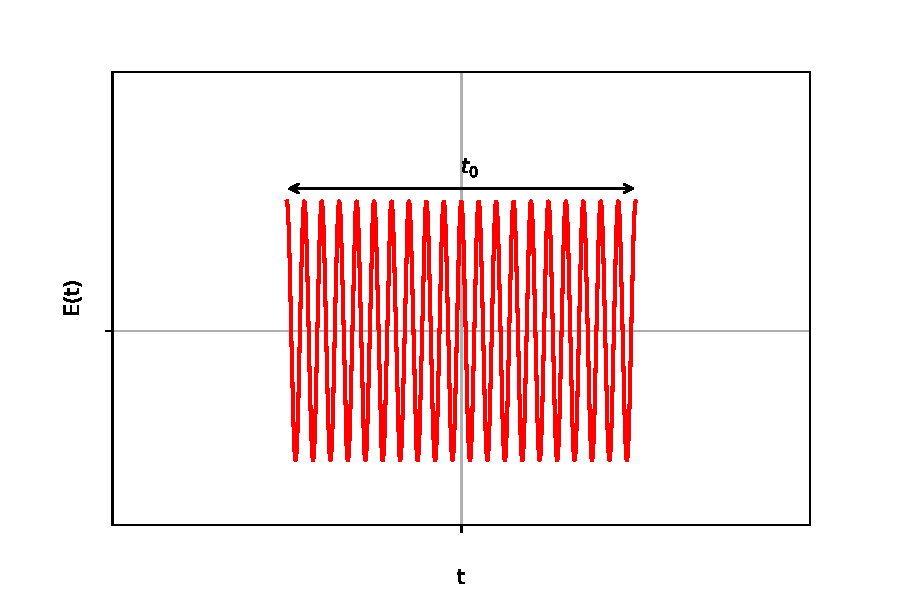
\includegraphics[scale=0.8]{02-Achura_espectral.pdf}
\end{figure}

Es evidente que dicho pulso tiene una frecuencia definida, tal que $E =E_0 \cos (\omega_c t - \epsilon) \ t \in [0,t_0]$. Para $t \notin [0,t_0] \ E(t)=0$. Supongamos ahora que queremos calcular $E(\omega)$, para ver luego calcular la intensidad $I(\omega)$:

\begin{equation}
E (\omega) = \int_{-\infty}^{\infty} \mathsf{E}(t) e^{i (\omega-\omega_c)t + \epsilon} \D t = \int_{0}^{t_0} \mathsf{E}(t) e^{i (\omega-\omega_c)t + \epsilon} \D t 
\end{equation}
si definimos $\omega_d = \omega-\omega_c$:

\begin{equation}
E(\omega) = \frac{e^{i \epsilon} \mathsf{E}_0 }{i \omega_d} (e^{i \omega_d t_0} -1)
\end{equation}
la intensidad definida como $I(\omega) = |E(\omega)|^2$ vendrá dada por:

\begin{equation}
I (\omega) = \mathsf{E}_0^2 \ t_0^2 \ \mathrm{senc} (\omega_d t_0 /2)
\end{equation}
Si definimos la \textbf{anchura espectral} $\Delta\omega$ como la relación para la cual $I(\omega\pm\Delta\omega)$ cae un $40\%$, tenemos que se verifica la relación:

\begin{equation}
\Delta \omega t_0 \approx 2 \pi
\end{equation}
es decir existe una relación intrínseca entre la duración de un pulso y la anchura espectral. Aunque esto solo se verifica para un pulso rectangular, es una buena aproximación para casi cualquier pulso. A partir de la anchura espectral definimos los siguientes conceptos:

\begin{itemize}
\item \textbf{Tiempo de coherencia:} ($\tau$) es el intervalo durante el cual la onda (especialmente un haz láser) puede ser considerada coherente, y viene dada por:

\begin{equation}
\tau = \dfrac{2 \pi}{\Delta \omega}
\end{equation}
el tiempo de coherencia no es mas que la duración del intervalo para el cual una onda se puede considerar monocromática, sinusoidal ideal. Por eso cuando $\Delta \omega \rightarrow 0$, el tiempo $t_0 \rightarrow \infty$, porque para una onda ideal un pulso de duración infinita tendrá una fase conocida. 

\item \textbf{Longiutd de coherencia}: ($l_0$) es la distancia de propagación sobre la que una onda coherente mantiene un grado especificado de coherencia, definido como:

\begin{equation}
l_0 = \dfrac{2 \pi}{\Delta \omega} c 
\end{equation}
la longitud de coherencia, al igual que el tiempo de coherencia tiene relación con la distancia para un timpo fijo para la cual la onda puede considerarse con fase inicial conocida (al igual que antes).

\item \textbf{Anchura cromática}: ($\lambda_0$) viene dada por:

\begin{equation}
\lambda_0 = \lambda_c^2 \Delta \omega / c
\end{equation}
\end{itemize}

\section{Coherencia Óptica}

\subsection{Función de coherencia}

Los campos producidos por fuentes reales presentan fluctuaciones estadísticas resultates de emisiones de pulsos finitos independientes entre sí, y de que los emisores puntuales de una fuente son independientes. Consecuentemente las ondas pierden idealidad, y dejan de estar correlacionadas entre sí. \\

Un campo puro es aquel que no presenta fluctuaciones de ningún tipo, de tal forma que el campo en dos puntos espacio-temporales (e-t) diferentes $(1)\equiv (\rn_1,t), (2)\equiv (\rn_2,t+\delta t)$ dan lugar a un promedio estadístico donde $$\langle \En_{(1)}^* \En_{(2)} \rangle_T = E_0^2 \langle  e^{i [\kn(\rn_2-\rn_1)-\omega \tau]} \rangle_T \tquad \En_{(1)}=\En (\rn_1,t) \quad \En_{(2)} = \En (\rn_2,t+\delta t)  $$ Ahora bien, de existir \textit{fluctuaciones aleatorias} en la fase inicial, amplitud o frecuencia, es obvio que dicho promedio sería diferente. En este contexto tenemos que definir algún parámetro que nos permita distinguir los campos puros de campos no puros, y el grado de ``pureza'' que presentan. La \textbf{función de coherencia} de primer orden $g_{(1)}$ nos da una medida de el grado de coherencia de una onda en dos campos ópticos, y se define como:

\begin{equation}
g_{(1)} (\rn_1,\rn_2,\delta t) = \frac{\langle \En_{(1)}^* \En\2 \rangle}{\langle \En\1\En\1 \rangle^{1/2}  \langle \En\2 \En\2^* \rangle^{1/2}} \label{Ec:02.04-1}
\end{equation} 
El promedio temporal, como ya veremos, será equivalente al promedio estadístico, ya que si tomamos un tiempo suficientemente largo las variaciones intrínsecas de la fuente habrán recorrido todas las posibilidades (incluso varias veces cada una de ellas). \\

Como podemos ver la función de coherencia es una \textit{función compleja}. Es muy interesante expresar la función de coherencia con un módulo y una fase, de tal modo que:

\begin{equation}
g_{(1)} (\rn_1,\rn_2,\delta t) = |g\1 (\rn_1,\rn_2,\delta t) | \cdot \exp  \parentesis{ i \alpha (\rn_1,\rn_2,\delta t)}
\end{equation}
Al módulo de la función de coherencia $|g\1|=g$ se le conoce como \textbf{grado de coherencia}, y en función de esto decimos que hay \textit{coherencia nula} ($g=0$), \textit{coherencia parcial} ($0 < g < 1$) o \textit{coherencia total} ($g=1$). \\

\subsection{Coherencia temporal}

La \textbf{coherencia temporal} es la correlación del campo óptico en dos instantes $t_1=t$ y $t_2=t+\delta t$, pero en el mismo punto $\rn$ (o en dos puntos fijos). Está asociado a la \textit{anchura espectral de la fuente}. Puede formalizarse usando pulsos de duración media $\tau$ (tiempo de coherencia) con fase inicial aleatoria. \\

Supongamos que queremos medir la coherencia temporal. Consideremos una \textit{fuente temporal policromática} de la que salen pulsos de duración media $\tau$. Seleccionamos también dos puntos $\rn_1$ y $\rn_2$ del frente de ondas. La mejor forma de medir la coherencia temporal será calcular varias medidas del campo para pares de instantes diferentes pero que entre ellos halla un mismo retardo. Luego podremos promediar el resultado obteniendo $g_{(1)}(\delta t_1)$. Luego iremos cambiando el retardo, obteniendo $g_{(1)}(\delta t_2),g_{(1)}(\delta t_3)...$. Con los suficientes puntos obtenemos $g(\delta t)$. Podemos implementar $\tau$ manteniendo entre los puntos una distancia $c \delta t_1...$

\subsection{Coherencia espacial}

La \textbf{coherencia espacial} es la correlación en dos puntos $\rn_1,\rn_2$ en el mismo instante $t$. Está asociada a \textit{dimensión de la fuente} $\Delta S$. Puede formalizarse usando pulsos grandes (con poca anchura espectral, casi monocromáticos), pero donde cada punto de la fuente emite pulsos de fase inicial aleatoria.  \\

Para poder calcular supondremos una fuente extensa $S$ casi-monocromática. Entonces mediremos el campo en pares de puntos espaciales ($\rn_1,\rn_2$),($\rn_1',\rn_2'$)... Si medimos el campo en el mismo instante temporal para todos estos, o midiendo con retardos iguales, obtendremos que $g\1 (\rn_1,\rn_2)$. Podremos entonces ver que la función de coherencia depende principalmente de la distancia entre los puntos. 

\section{Estadística equiprobable}

Como podemos fijarnos, existe una relación entre el índice de correlación estadístico $r$ y la función de coherencia $g\1$. Recordando la definición de $r$:

\begin{equation}
r=\frac{\frac{1}{N}\sum (x_i - \overline{x})(y_i-\overline{y})}{\sqrt{ \frac{1}{N}\sum (y_i-\overline{y})^2} \sqrt{ \frac{1}{N}  \sum (x_i - \overline{x})^2}}
\end{equation}
vemos que es muy parecida a \ref{Ec:2.04-1} si $\overline{x},\overline{y}=0$ y si hacemos a las variables \textit{variables complejas}. Por tanto es comprensible decir que la función de coherencia la podemos relacionar con promedios estadísticos. Entonces es interesante estudiar las distribuciones de probabilidad más interesantes, como puede ser la \textit{distribución equiprobable}. Sea la función de probabilidad:

\begin{equation}
P (\gamma_a) = \left\lbrace
\begin{array}{cl}
\frac{1}{2 \Delta \gamma_0} & \quad \gamma_a \in [-\Delta \gamma_0,\Delta \gamma_0] \\
0 & \quad \gamma_a \notin [-\Delta \gamma_0,\Delta \gamma_0]
\end{array}
\right.
\end{equation}
Calcular el valor medio de cualquier función de $\gamma_a$, una vez conocida la distribución de probabilidad, es tan trivial como lo sea la integral correspondiente. Aunque de momento estemos hablando únicamente de estadística, al lector le puede resultar interesante calcular el valor medio de la función compleja $e^{i q \gamma_a}$:

\begin{equation}
\langle e^{i q \gamma_a} \rangle = \int e^{i q \gamma_a}  P(\gamma_a) \D \gamma_a = \frac{1}{2 \Delta \gamma_0} \int_{-\Delta \gamma_0}^{\Delta \gamma_0} e^{i q \gamma-a} \D \gamma_a = \dfrac{e^{i q \Delta \gamma_0} -e^{-i q \Delta \gamma_0} }{2 \Delta \gamma_0 i q } = \mathrm{sinc} (q \Delta \gamma_0)
\end{equation}
Otras funciones interesantes pueden ser $\sin (\gamma_a), \cos (\gamma_a)$ o $\cos^2 ( \gamma_a),\sin^2(\gamma_a)$. Un lector perspicaz puede ver la gran utilidad de este promedio: si por ejemplo $\gamma_a$ fuera la fase inicial, y supusieramos que una fuente emite durante un tiempo $\Delta t$ fases iniciales aleatorias de manera equiprobable, el promedio temporal coincidiría con el promedio estadístico.  

\section{Teoría general de la interferencia}

\subsection{Forma general de la interferencia}

Supongamos que en el mismo puntos espacio-temporales dos (o varias) ondas electromagnéticas diferentes $\En_1,\En_2$ pero con la misma frecuencia (expresión general $\En_i = \Encal_i e^{-i\omega t}$), que además verifican que $\nabla \mathcal{L}_1 \approx \nabla \mathcal{L}_2 \approx \nabla \mathcal{L}$ (llamado \textit{proximidad de la fase local}), se superponen. En ese caso $\En_T = \En_1 + \En_2$. Aunque los campos sean aditivos, las irradiancias no (en general $I_T \neq I_1 + I_2$). La expresión de la irradiancia total viene dada por:

\begin{equation}
I (\rn,t) = \langle \En_1 \En_1^* \rangle  + \langle \En_2 \En_2^* \rangle  + 2  \langle  \Real (\En_2 \En_1^*) \rangle  \label{Ec:02.06-1}
\end{equation}
Llamamos como \textit{intensidad incoherente} a la intensidad $I_{inc}=I_1+I_2$, ya que es la única que se ve cuando el grado de coherencia es nulo; y \textit{intensidad coherente} $I_{coh} = 2 \langle  \Real (\En_2 \En_1^*) \rangle  $, ya que es propia de un sistema donde hay interferencia. En ese caso tenemos que:

\begin{equation}
I = I_1 + I_2 + 2  \langle  \Real (\En_2 \En_1^*) \rangle 
\end{equation}

\subsection{Forma normal de la coherencia} 

Si nos fijamos, la ecuación \ref{Ec:02.06-1}, es común escribir la intensidad total en lo en la literatura se llama la \textbf{forma normal}:

\begin{equation}
I = \parentesis{\langle \En_1 \En_1^* \rangle  + \langle \En_2 \En_2^* \rangle } \ccorchetes{1 + \frac{2  \langle  \Real (\En_2 \En_1^*) \rangle  }{\langle \En_1 \En_1^* \rangle  + \langle \En_2 \En_2^* \rangle }}
\end{equation}
que si nos fijamos implementa, indirectamente, la función de coherencia, ya que $g\1 \propto \langle  \En_2 \En_1^* \rangle$. Usando las intensidades la forma normal:

\begin{equation}
I = (I_1+I_2)\ccorchetes{1+\frac{2 \langle \Real (\En_2 \En_1^* ) \rangle  }{I_1 + I_2}}
\end{equation}



\subsection{Interferencia de ondas localmente planas}

En general las ondas que estudiaremos serán ondas localmente planas, con una polarización cualquiera, una fase inicial cualquiera, emitidas en posiciones diferentes. Lo único que van a compartir será la frecuencia y la dirección de propagación de la energía. En ese caso tenemos que la expresión mas general de la onda electromagnética:

\begin{equation}
\En_i = \mathsf{E}_i e^{i(k_0 \mathcal{L}_i - \omega_c t)} e^{i \epsilon_i} \un_i
\end{equation}
Si estudiamos ahora la forma de la \ref{Ec:02.06-1} en este caso particular, tendremos que:

\begin{equation}
I(\rn) = \parentesis{I_1+I_2}\ccorchetes{1+2\frac{\sqrt{I_1 I_2}}{I_1+I_2} \cos (\Phi)}
\end{equation}
En $\Phi$, la llamada \textbf{fase interferencial}, se incluirá: la diferencia de las fases iniciales ($\epsilon \equiv \epsilon_2 - \epsilon_1$), la diferencia de fase que se produce al recorrer distancias diferentes y la diferencia de fase producida por las distintas polarizaciones de las ondas ($\epsilon'\equiv \arg (\un_1^* \un_2)$) . En ese caso:

\begin{equation}
\Phi (\rn) = k_0 [\mathcal{L}_2 (\rn) - \mathcal{L}_1 (\rn)] + \epsilon + \epsilon' =  k_0  \Delta + \epsilon + \epsilon'  \label{Ec:02.05-01-Fase}
\end{equation}
Al término real que acompaña al coseno de la fase interferncial se le llama \textbf{visibilidad} o \textbf{contraste}, y se denota por $\mathcal{V}$, tal que:

\begin{equation}
\mathcal{V} = \frac{2 \sqrt{I_1 I_2} }{I_1 + I_2} (\un_1^* \cdot \un_2) \label{Ec:02.05-02-Visibilidad}
\end{equation}
pudiendo tener valores entre 0, y 1. Es lógico que a mayor visibilidad la diferencia entre los máximos y mínimos de $I(\rn)$ será máxima. Cuando la visibilidad es mínima no existen mínimos y máximos interferenciales (las intensidades son aditivas y no hay interferencia). Entones la \textbf{expresión normal} será:

\begin{equation}
I(\rn) = (I_1 + I_2) \ccorchetes{ 1 + \mathcal{V} \cos (\Phi)}
\end{equation}
Resumiendo los conceptos:

\begin{itemize}
\item \textbf{Visibilidad} ($\mathcal{V}$). La visibilidad es un parámetro que nos relaciona directamente la cantidad de interferencia que hay entre dos ondas. Ver ecuación \ref{Ec:02.05-02-Visibilidad}. 
\item \textbf{Fase interferencial} ($\Phi$). La fase interferencial es la principal fuente de la interferencia. Nos dice en que regiones se encuentran los máximos, y mínimos. En general regula el \textit{patrón interferencial}, ya que las regiones de fase constante son exactamente iguales a las regiones de intensidad constante (por construcción). Ver ecuación \ref{Ec:02.05-01-Fase}. 
\item \textbf{Geometría interferencial}. La geometría interferencial es la forma que tienen los patrones máximos y mínimos. Si por ejemplo los máximos son lineas rectas decimos que su geometría es lineal, y si son circunferencias decimos que su geometría es circular. Si la geometría depende de las 3 dimensiones decimos que la interferencia es \textbf{localizada}. En cualquier otro caso decimos que es \textbf{no localizada}.
\item \textbf{Interfranja} ($i$). Es la distancia entre mínimos (o máximos) consecutivos. Existen patrones para los cuales la interfranja no es constante, y depende del máximo o mínimo estudiado. 
\end{itemize}

\section{Métodos de interferencia}

La condición para tener  \textit{interferencia ideal} es producir dos campos o mas de igual frecuencia $\omega_c$ mutuamente coherentes, es decir, que la fase entre ambas esté completamente realcionadas. Es decir: $\langle E_1^* E_2 \rangle \varpropto g\1 \neq 0$. Esta condición sugiere que los campos que se construyan a partir de la división de un campo principal serán campos mutuamente coherentes. Los métodos mas comunes son: \textbf{división de la frente de onda} (DFO) y la  \textbf{división simple de amplitud} (DSA). Un ejemplo de un divisor de frente de onda es un retardador de fase $\Delta \Phi$.

\section{Interferencia por División del Frente de Onda}

\subsection{Interferómetro de Young}

El interferómetro de Young es un objeto que permite crear interferencia de una gran calidad (alta visibilidad). En la figura \ref{Fig:02.07-1} podemos ver como se construye: lo que hacemos es poner una pantalla delante de la onda recibida, con dos agujeros. Según el \textit{principio de Huygens} se formará un nuevo frente de ondas esférico en cada una de los agujeros, de tal modo que si colocamos una pantalla delante de ellas veremos como interfieren. \\

\begin{figure}[h!] \centering
\includegraphics[scale=0.1]{02-Young.pdf}
\caption{interferómetro de Young.} \label{Fig:02.07-1}
\end{figure}

Una vez entendemos lo que tenemos que hacer, en realidad solo quedan hacer ejercicios, ya que la teoría vista hasta ahora nos permite calcular todo: diferencias de fase, amplitudes, retardos... Lo único que debemos tener en cuenta a mayores es lo siguiente: al pasar un agujero o una franja la amplitud se ve dividida, debido a los fenómenos de difracción, por un factor $i \lambda$ (agujero) o $\sqrt{i\lambda}$ (franja). Una vez tenemos en cuenta esto podemos resolver cualquier problema de este tipo: onda incidente plana, onda incidente esférico-paraxial con fuente principal $(u,0,-L)$, con polarizadores tras los agujeros, con láminas retardadoras...  A continuación presentaremos los ejercicios mas comunes: \\


\shadowbox{\textbf{Onda plana incidente}} 

\hrulefill

Sea una onda plana incidiendo en el un plano opaco con dos aperturas muy pequeñas (figura \ref{Fig:02.07-1}). Obviamente el campo en ambas aperturas será mutuamente coherente, ya que las ondas están intrínsecamente relacionadas. Por cada apertura (siguiendo el principio de Huyegns) de formará un nuevo frente de ondas esférico. Sea el agujero el que se encuentra (1) se encuentra en (d/2,0,0) y el agujero (2) en (-d/2,0,0). Como la onda es una onda plana, el campo incidente en (1) y en (2) será exactamente el mismo. Si suponemos que medimos la interferencia en un punto muy lejano:

\begin{equation}
\mathcal{E}_{\binom{(1)}{(2)}} = \dfrac{E_0}{(i \lambda_0)z} e^{ikz} e^{ik\frac{(x\mp d/2)^2+y^2}{2z}}
\end{equation}
donde $E_0$ es la amplitud de la onda plana (la incidente). Si nuestro plano se encuentra a una distancia $D$, tendremos que en dicho punto los campos valdrán:

\begin{equation}
\mathcal{E}_{\binom{(1)}{(2)}} (x,y,D) = \dfrac{E_0}{(i \lambda_0)D} e^{ikz} e^{ik\frac{(x\mp d/2)^2+y^2}{2D}} e^{i \epsilon}
\end{equation}
Es obvio que la diferencia de fase $\Phi = k \frac{ x d}{D}$. Entonces la intensidad, si $I_0=E_0^2$:

\begin{equation}
I(\rn) = \frac{2I_0^2}{\lambda_0^2 D^2} \ccorchetes{1+\cos \parentesis{k\frac{x d}{D}}}
\end{equation}
Estudiemos ahora la geometría interferencial y el tamaño de las interfranjas. Es evidente que las regiones donde $\Phi$ es constante definen rectas en el espacio. En particular son rectas de $x$ constante. Entonces una onda plana incidente a través de un interferómetro de Young produce un patrón interferencial lineal. Buscamos los máximos y mínimos:

\begin{equation}
x_{\max} = (2n\pi) \frac{D}{kd} \tquad 
x_{\min} = (2n+1)\pi \frac{D}{kd} \tquad n=0,1,2...
\end{equation}
Donde está claro que la distancia $i$ (interfranja) entre mínimos viene dada por:

\begin{equation}
i = 2 \pi \frac{D}{kd} = \dfrac{\lambda_0 D}{d}
\end{equation}
aunque sea evidente, este patrón interferencial es un patrón no localizado, ya que en cualquier plano $z$ se verá este patrón. Quizás no con la misma intensidad, ya que la onda pierde fuerza a medida que la distancia crece, pero si conservará $i$, o la visiblidad $\mathcal{V}=1$. 


\hrulefill \\

\shadowbox{\textbf{Onda plana incidente: no perpendicular}} 

\hrulefill 

Supongamos ahora que la plana no incide perpendicularmente al plano opaco. Entonces es evidente que existirá la onda incidente en el agujero 1 será diferente a la del agujero 2 en una fase relacionada con la diferencia de camino óptico entre ambos puntos. Si el plano se encuentra en $z=0$, y el ángulo de incidencia de la onda es $\alpha$, tendremos que la diferencia de fase vendrá dada por la diferencia de camino óptico:

\begin{equation}
\Delta \mathcal{L} = d \cos (\alpha)
\end{equation}
Entonces a la ejercicio anterior solo tendremos que añadir esta diferencia de fase: el resto será completamente análogo:

\begin{equation}
\Phi = k \frac{xd}{D} +  d \cos (\alpha)
\end{equation}
Si nos fijamos la interfranja no variará: seguirá siendo válida $i=2D/kd$. Lo único que haremos es desplazar los máximos y mínimos de posición.

\hrulefill \\


\shadowbox{\textbf{Onda esférico paraxial: caso simple}} \\

\hrulefill

Supongamos una onda esférico-paraxial que parte de un punto (0,0,-L). Por el resto el problema será igual que los dos anteriores: dos agujeros situados en $x=\pm d/2$. Lo primero que debemos preguntarnos es como es la onda incidente en los puntos (1),(2). Está claro que la onda trasmitid por cada agujero (1),(2); viene dada por (recordemos que z=0):


$$  E\1 = \frac{A_{o} / (i \lambda_0)}{L+z} e^{i\frac{(d/2)^2}{-2L}} e^{i \epsilon} e^{ikz} e^{ik\frac{(x - d/2)^2+y^2}{2z}} \quad
E\2 = \frac{A_{o} / (i \lambda_0)}{L+z} e^{i\frac{(d/2)^2}{-2L}} e^{i \epsilon} e^{ikz} e^{ik\frac{(x + d/2)^2+y^2}{2z}} $$
es decir, la \textit{fase interfernecial} $\Phi$ es análoga al caso de una onda plana incidiendo con un ángulo:
$$ \Phi = k \frac{xd}{D} $$
y por tanto la geometría se conserva (geometría interferencial lineal) y la interfranja tampoco:

$$ i = \frac{2 \pi D}{kd} = \dfrac{\lambda_0 D}{d} $$
 

\hrulefill \\

\shadowbox{\textbf{Onda esférico paraxial: caso mas general}} \\

\hrulefill 

Supongamos una onda esférico-paraxial que parte de un punto ($\pm u,0,-L$). Por el resto el problema será igual que los dos anteriores: dos agujeros situados en $x=\pm d/2$. Lo primero que debemos preguntarnos es como es la onda incidente en los puntos (1),(2). Está claro que la onda incidente en el agujero (1) viene dada por (recordemos que z=0):


$$  E\1 = \frac{A_{o} / (i \lambda_0)}{L+z} e^{i\frac{(-u+d/2)^2}{-2L}} e^{i \epsilon} e^{ikz} e^{ik\frac{(x - d/2)^2+y^2}{2z}}  \quad
E\2 = \frac{A_{o} / (i \lambda_0)}{L+z} e^{i\frac{(-u-d/2)^2}{-2L}} e^{i \epsilon} e^{ikz} e^{ik\frac{(x + d/2)^2+y^2}{2z}} $$
es decir, la \textit{fase interfernecial} $\Phi$ sigue siendo igual que el caso de una onda plana, esto es:

$$ \Phi = k \frac{xd}{D} + k \frac{ud}{L} $$
y por tanto la geometría se conserva (geometría interferencial lineal), lo único que pasa es que los mínimos/máximos se mueven de posición. El desplazamiento de un mínimo será:

$$ \Delta x = - k \frac{ud}{L} $$
que es donde ahora está el máximo principal. Es decir, el máximo se desplazo hacia la región contraria de donde desplazamos el punto paraxial. 

\hrulefill \\


\subsection{Interferómetros tipo Young}

\shadowbox{\textbf{Polarizadores}} \\

\shadowbox{\textbf{Biprisma de Fresnel}} \\


\section{Función de Coherencia Espacial}

\subsection{Fuente extensa}

Sean dos fuentes puntuales mutuamente \textit{incoherentes} de frecuencia $\omega$ y factores de amplitud $A_{u_i}$ con $i=1,2$, situados en los puntos $(u,v) = \lbrace (u_1,0),(u_2,0) \rbrace$ del plano $z=-L$ polarizados en el eje $y$. Si dichos puntos iluminan un interferómetro de Young con sus agujeros en los puntos $(d/2,0,0)$ y $(-d/2,0,0)$, con coeficientes de trasmisión $t_b$. En ese caso tendremos que el campo óptico total en un plano $z=D$, viene dado por:

\begin{equation}
\Encal = \Encal_{u_1} e^{i \gamma_{a_1}} + \Encal_{u_2} e^{i \gamma_{a_2}} = (\Encal_{1u_1} + \Encal_{2u_1} )e^{i \gamma_{a_1}} + ( \Encal_{1u_2} +\Encal_{2u_2} ) e^{i \gamma_{a_2}}
\end{equation}
donde las fases $\gamma_{ai}$ son completamente aleatorias. Entonces la intensidad vendrá dada por:

\begin{equation}
I = \langle | \Encal_{u_1} e^{i \gamma_{a_1}} + \Encal_{u_2} e^{i \gamma_{a_2}} |^2 \rangle = |\mathcal{E}_{u_1}|^2 + |\mathcal{E}_{u_2}|^2 + 2 \Real \langle \mathcal{E}_{u_1} \mathcal{E}_{u_2}^* e^{i \gamma_a} \rangle = I_{u_1} + I_{u_2}
\end{equation}
es decir, para dos fuentes mutuamente incoherentes \textit{la intensidad total es la suma de las intensidades interferenciales}. Tengamos en cuenta que $\gamma_a=(\gamma_{a1} - \gamma_{a2})$. Entonces la intensidad total vendrá dada por:

\begin{equation}
I = 2 I_{o1} \ccorchetes{ 1 + \cos \parentesis{\frac{k_0 xd}{D} + \frac{k_0 u_1 d}{L}}} + 2 I_{o2} \ccorchetes{ 1 + \cos \parentesis{\frac{k_0 xd}{D} + \frac{k_0 u_2 d}{L}}} \label{Ec:02.08-23}
\end{equation}
Esto lo hemos hecho para \textit{dos fuentes mutamente incoherentes}. Si generalizamos el caso para $N$ fuentes mutuamente incoherentes es evidente que $I=\sum_1^N I_{u_i}$. De este modo podemos generalizar el caso para una \textbf{fuente extensa}, con una densidad de intensidad $i_L (u,v) \approx A_o^2 (u,v) /L^2$, tendremos que:

\begin{equation}
I(x) = \int 2 i(u) \ccorchetes{ 1 + \cos \parentesis{\frac{k_0 xd}{D} + \frac{k_0  ud }{L}}} \D u \tquad i(u) =  \frac{i_L (u)}{\lambda_ 0^2 D^2} = \frac{A_0^2(u,v)}{\lambda_0^2 L^2 D^2}
\end{equation}
donde por simplicidad hemos tomado $t_{b1} = t_{b2} = t_b = 1$. Por tanto hemos llegado al patrón de interferencia para una fuente extensa. Esto se puede usar para, por ejemplo, calcular la ditancia entre dos estrellas en un sistema binario. \\

\shadowbox{\textbf{Interferómetro estelar de Michelson}}

\hrulefill \\

Supongamos que tenemos dos puntos luminosos en $u_1=u_0$ y en $u_2=-u_0$ equienergéticos (igual intensidad $i_0 = A_0^2/L^2$). Supongamos que entre nuestros dos agujeros hay una distancia $d$. En ese caso según la ecuación \ref{Ec:02.08-23} la intensidad:

\begin{eqnarray*}
 I  & = & 2 \frac{A_0^2}{\lambda_0^2 L^2 D^2} \ccorchetes{ 1 + \cos \parentesis{\frac{k_0 xd}{D} + \frac{k_0 u_0 d}{L}}} + 2 \frac{A_0^2}{\lambda_0^2 L^2 D^2} \ccorchetes{ 1 + \cos \parentesis{\frac{k_0 xd}{D} - \frac{k_0 u_0 d}{L}}} =  \\
 & = & 4 I_0 \ccorchetes{ 1 + \cos \parentesis{\frac{k_0 xd}{D} } \cos \parentesis{\frac{k_0 u_0 d}{L}}} 
\end{eqnarray*}
con $I_0 = A_0^2 / \lambda_0^2 D^2 L^2$. Como podemos ver el grado de coherencia o visibilidad viene dado por $\mathcal{V} = | \cos (k_0 u d / L ) |$, habiendo zonas negras y zonas mas blancos/grises. Es notable darse cuenta que de esta forma podemos transformar un problema que involucra ondas mutuamente incoherentes en un problema que equivalente a uno con una onda coherente (si $k_0 u d / L = 2n\pi$).



\hrulefill


\subsection{Fuente extensa y función de coherencia}

Queremos escribir la función $I(x)$ para una fuente extensa pero en forma normal. Para esto es necesario crear unos nuevos coeficientes, que serán:

\begin{equation}
\Phi = \frac{k_o d x }{D} = \omega \tau \tquad \beta (u) = \frac{k_0 d u }{L} \tquad Q = 2 \int_{-u_0}^{u_0} i(u) \D u  \label{Ec:02.08-01}
\end{equation}
\begin{equation}
C = 2 \int_{-u_0}^{u_0} i(u) \cos(B(u)) \D u \tquad S = 2 \int_{-u_0}^{u_0} i(u) \sin (B(u)) \D u \label{Ec:02.08-02}
\end{equation}
Si tenemos en cuenta la relación trigonométrica $\cos (A+B) = \cos (A)  \cos (B) - \sin (A) \sin (B)$, podemos llegar a conclusión de que:

$$ I(x) = \int \ccorchetes{ 2 i (u) + 2 i(u) \cos \parentesis{\beta(u)} \cos \parentesis{\Phi} - 2 i(u) \sin \parentesis{\beta(u)} \sin \parentesis{\Phi}} $$
es decir, escrito en función de los coeficientes \ref{Ec:02.08-01} y \ref{Ec:02.08-02} tenemos que la intensidad

\begin{equation}
I (x) = Q + C \cos (\Phi) - S \sin (\Phi) 
\end{equation}
y ahora si, si definimos los parámetros visibilidad $\mathcal{V}$ y ángulo $\alpha$ como

\begin{equation}
\mathcal{V} = \dfrac{\sqrt{C^2+S^2}}{Q} \tquad \cos (\alpha)=\frac{C}{\sqrt{C^2+S^2}} \tquad \sin (\alpha) = \frac{S}{\sqrt{C^2+S^2}}
\end{equation}
En ese caso la intensidad para una fuente extensa tendrá el valor de:

\begin{equation}
I(s) = Q [1 + \mathcal{V} \cos (\Phi + \alpha)]
\end{equation}
En general $\mathcal{V}<1$, siendo el origen la incoherencia mutua de los puntos de la fuente extensa. Representa el \textbf{grado de coherencia espacial}. El restultado equivale a dos campos procedentes de agujeros de igual $I_0=Q/2$ y \textit{parcialmente coherentes}. \\

\shadowbox{\textbf{Fuente lineal de dimensión $2u_0$}} 

\hrulefill

Si nuestra fuente lineal incoherente de dimensión $2u_0$, paralelo al eje de los agujeros, tiene una distribución uniforme de velocidad tal que

$$ i_L (u) = \left\lbrace 
\begin{array}{lc}
0 & - \infty < u < -u_0 \\
i_0 = \frac{A_0^2}{L^2} & -u_0 < u < u_0 \\
0  & u_0 < u < \infty \\
\end{array}
\right. $$
En ese caso es obvio que al salir de las franjas la intensidad tendrá un valor de:

$$ i (u) = t_b^2 \frac{i_0}{\lambda_0^2 D^2} $$
Lo único que tenemos que hacer son las integrales dadas por las ecuaciones \ref{Ec:02.08-01} y \ref{Ec:02.08-02}. No son en absoluto complicadas, ya que $i(u) = \cte$. Directamente:

$$Q = 2  \parentesis{\frac{2t_b^2 u_0^2 i_o}{\lambda_0^2 D^2}} =2 I_0$$
$$C  = \int 2 i(u) \cos (\beta u) \D u = 2 I_0 \frac{\sin (\beta u_0)}{\beta u_0} \tquad S = 0 $$
es evidente que $S=0$, ya que el seno es una función impar y la intensidad es una función lineal. En ese caso tendremos que nuestra intensidad:

$$ I(x) = 2I_0 \ccorchetes{1+\mathrm{senc} (\beta u_0) \cos (\omega \tau)} $$
es decir nuestra visibilidad o grado de coherencia viene determinada por la expresión:

$$ \mathcal{V} = |g\1|=|\mathrm{senc} (\beta \mu_0)| $$
donde si $u_0\rightarrow 0$ recuperamos $\mathcal{V}=1$, como debería ser. El valor $\mathcal{V}$ es el resultado del desplazamiento mutuo de padrones interferenciales producidos por puntos mutuamente coherentes.

\hrulefill \\

Como hemos podido ver en el ejemplo anterior la coherencia espacial de una perturbación depende del criterio que hagamos para definir que es una onda mutuamente coherente. Si $\mathcal{V} = |\sinc (k_0 d u_0 /L)|$, tenemos que podemos suponer que la onda es mutuamente coherente hasta el prime cero, o cuando la visiblidad cae $2/\pi$. El criterio es completamente arbitrario. \\

Si escogemos que el argumento  $\theta_c = k_0 d u_0 /L$ (arbitrariamente) como aquel que nos da el valor para el cual la onda se puede considerar mutuamente coherente. Sin embargo no nos importa el argumento, nosotros queremos obtener un valor tangible, que podamos medir en el laboratorio, como puede ser una \textit{distancia} o un \textit{tiempo}. Despejando la anchura $d=d_c$:

\begin{equation}
d_c = \frac{\theta_c L \lambda_0}{2 \pi u_0}
\end{equation}
siempre que $d<d_c$ la perturbación es coherente. Siempre que $L$ aumenta la anchura de coherencia $d_c$ aumenta, y la perturbación en $z=0$ tiene mas dominio de la coherencia.

\section{Teorema de Van Cittert-Zernike}
\subsection{Introducción al Teorema VC-Z}

El \textbf{teorema de Van Cittert-Zenike} (VC-Z) nos dice que si $i(u)$ es una función par, la intensidad $i(u)$ se relaciona directamente con la función $F(d)=C(d)/Q = |g\1| (d,\tau)$ mediante la \textit{Transformada de Fourier Coseno} (TFC) tal que ($i_n(u)$ es la intensidad normalizada):

\begin{equation}
i_n (u) \varpropto \int F(\beta) \cos (\beta u) \D \beta
\end{equation}
Es decir si somos capaces de obtener el grado de coherencia o visibilidad podremos obtener la distribución de intensidad de un objeto luminoso. Un lector perspicaz puede hallar el valor astronómico que tiene este teorema. Una vez determinada $F(\beta)$ solo habrá que para diferentes $\beta$, solo habrá que determinar la integral por medios evidentemente numéricos. De este modo podremos obtener la imagen del objeto. A esta técnica para obtener las imágenes se llama \textbf{imagen interferométrica}. 

\subsection{Función de coherencia y Teorema de VC-Z 1D} 

El teorema de Van Cittert-Zernike parte de la expresión de la función de coherencia espacial. La función de coherencia espacial $g\1 (\rn_1,\rn_2) $ viene dada por:

\begin{equation}
g\1 = \frac{\sqrt{C^2+S^2}}{Q} e^{i \arctan (S/C)} 
\end{equation}
de tal modo que la densidad de intensidad $i(u)$ producida por una fuente lineal viene determinada por la transformada de Fourier de la función de coherencia:

\begin{equation}
i_n (u) = \int |g\1|e^{ik_0\frac{du}{L}} \D d
\end{equation}
Este es el importantísimo \textbf{teorema de Van Cittert-Zernike} en una dimensión, vital para la observación de objetos astronómicos.

\subsection{Teorema de VC-Z 2D}

En general nosotros no vamos a saber si una distribución de intensidades es par o impar (ya que la gracia es de hecho obtenerla usando VC-Z). En ese caso tendremos que expandir a una transformada de Fourier, a poder ser en dos dimensiones. Entonces si nustra intensidad en dos dimensiones viene determinada por:

\begin{equation}
I(x,y) = Q \ccorchetes{ 1 + \mathcal{V} \cos (k_0 x d_x /D + k_0 d_y y / D + \alpha) }
\end{equation}
donde

\begin{equation}
Q = 2 \int i(u,v) \D u \D v \quad (C,S) = 2  \int i(u,v) (\cos,\sin) (k_0 d_x xu/L + k_0 d_y v / L)\D u \D v
\end{equation}
La expansión natural del teorema de Van Cittert-Zernike a dos dimensiones y a una transformada de Fourier se corresponde a:

\begin{equation}
i_n (u,v) = \int g\1 (u,v) e^{ i k_0 d_x u /L} e^{ i k_0 d_y v/L} \D d_x \D d_y
\end{equation}
\begin{equation}
g\1 (d_x,d_y) = \int  i_n (u,v)e^{ -i k_0 d_x u /L} e^{- i k_0 d_y v/L} \D u \D v
\end{equation}
a este teorema en realidad se llama \textbf{Teorema de Van Cittert-Zernike de campo alejado}. 

\section{Función de coherencia temporal}
\subsection{Interferencia policromática}

Si un interferómetro de Young es iluminado con una fuente espacialmente coherente pero policromática, la intensidad dependerá de la frecuencia, tal que la intensidad interferencial:

\begin{equation}
I(x) = \int I(\omega) \D \omega = \int 2 I_0 (\omega) \ccorchetes{1 + \cos (\omega x d / cD)}\D \omega
\end{equation}
que lógicamente da como resultado una intensidad de coherencia que va con un seno cociente (sinc). Luego todas las frecuencias tienen un máximo en el cero y un mínimo muy próximo, por lo que el máximo será de color blanco y el mínimo de tonos negro-marrón. Luego cada color tendrá un máximo/mínimo diferente. 

\subsection{Forma normal de la intensidad}

Sea una fuente principal puntual y policromática. Está claro que el patrón interferencial para cada frecuencia será diferente, generando así un patrón interferencial multicolor. Lógicamente podremos generalizar lo visto para la coherencia espacial pero ahora para la frecuencia, o lo que es lo mismo, el número de onda. Entonces tenemos que:

\begin{equation}
I(x) = \int 2 i(k_0) [1 + \cos (k_0 d x / D)] \D k_0 \tquad i(k_0) \approx i_L (k_0) / \lambda_c^2 D^2
\end{equation}
sea $k_d = (k_0 - k_c)$, donde $\omega_c$ es la frecuencia central. En ese caso, si $\Delta = xd /D = c \tau$:

\begin{equation}
I (x) = \int_{-\infty}^{\infty} 2 i (k_d) \ccorchetes{1+\cos[(k_d+k_c)\Delta]} \D k_d
\end{equation}
si ahora tenemos que $\Phi = k_c \Delta$ y $\tilde{B} = k_d \Delta$, podemos definir nuestros coeficientes $Q,S,C$ pero para la coherencia temporal. Para diferenciarlos les podremos una tilde encima:

\begin{equation}
\tilde{Q} = 2 \int i(k_d) \D k_d \tquad \tilde{C} = 2 \int i(k_d) \cos \tilde{B} \D k_d \tquad \tilde{S}=2\int i(k_d) \sin \tilde{B} \D k_d
\end{equation}
tal que:

\begin{equation}
I(x) = \tilde{Q} + \tilde{C} \cos (\Phi) - \tilde{S} \sin (\Phi) = \tilde{Q} \ccorchetes{1+\tilde{\mathcal{V}} \cos (\Phi + \tilde{\alpha}}
\end{equation}
donde $\tilde{\mathcal{V}}=\sqrt{\tilde{C}^2+\tilde{S}^2}/\tilde{Q}$, con $\cos (\tilde{\alpha}) = \tilde{C} / \sqrt{\tilde{C}^2 + \tilde{S}^2}$ y  $\sin (\tilde{\alpha}) = \tilde{S} / \sqrt{\tilde{C}^2 + \tilde{S}^2}$. Lógicamente ahora el valor $\tilde{\mathcal{V}}$, al igual que antes, representará el \textbf{grado de coherencia temporal} de una onda policromática. 

\newpage

\subsection{Teorema de Wiener-Khintchine}

Este teorema no es mas que la expresión del teorema de Van Cittert-Zernike pero en el dominio temporal. Esto es:

\begin{equation}
g\1 (\tau) = \int i_n (k_d) e^{ik_d c \tau} \D k_d
\end{equation}
donde $\tau = xd/cD$. La expresión usando la transformada inversa de Fourier nos permite obtener la expresión de la intensidad frecuencial:

\begin{equation}
i_n (k_d)  = \int g\1 (\tau) e^{-ik_d c \tau} \D \tau
\end{equation}

\newpage

\chapter{Interferencia por división simple de amplitud}

En la primera parte de este tema vamos a estudiar la interferencia por División Simple de Amplitud en láminas ópticas de espesor constante, presentando especial atención a su fenomenología y fomralización ondulatoria. En la segunda sección presentaremos la interferencia en lámidas de espesor variable. En la tercera y cuarta estudiaremos el interferómetro de Michelson y el de Mach-Zehnder, ambos de muy alto interés para la física fundamental y aplicada. En la quinta sección haremos una breve introducción a la interferencia óptico cuántica.  

\section{División Simple de Amplitud }

\subsection{Estudio casi ondulatorio}



Sea una lámina óptica de espesor constante $d$, o lámina plano paralela, en el vacío con un índice $n$. Supongamos que la iluminamos con una fuente $S$ natural, despolarizada y extensa (espacialmente incoherente), casi monocromática de frecuencia $\omega = k_0 c$. La luz incidente al contactar con la primera superficie generará dos ondas diferentes, una onda reflejada $\Ecal_{r1} = r \Ecal_i$ y una onda trasmitida $\Ecal_{t}=t\Ecal_i$. La onda trasmitida, al llegar a la primera superficie, puede o bien reflejarse de nuevo o trasmitirse. La onda reflejada al llegar de nuevo a la primera superficie puede o bien volver a reflejarse o trasmitida. Es entonces cuando obtenemos la segunda onda reflejada $\Ecal_{r2} =t'r't$. En la figura \ref{Fig:03.1-01}

\begin{figure}[h!] \centering
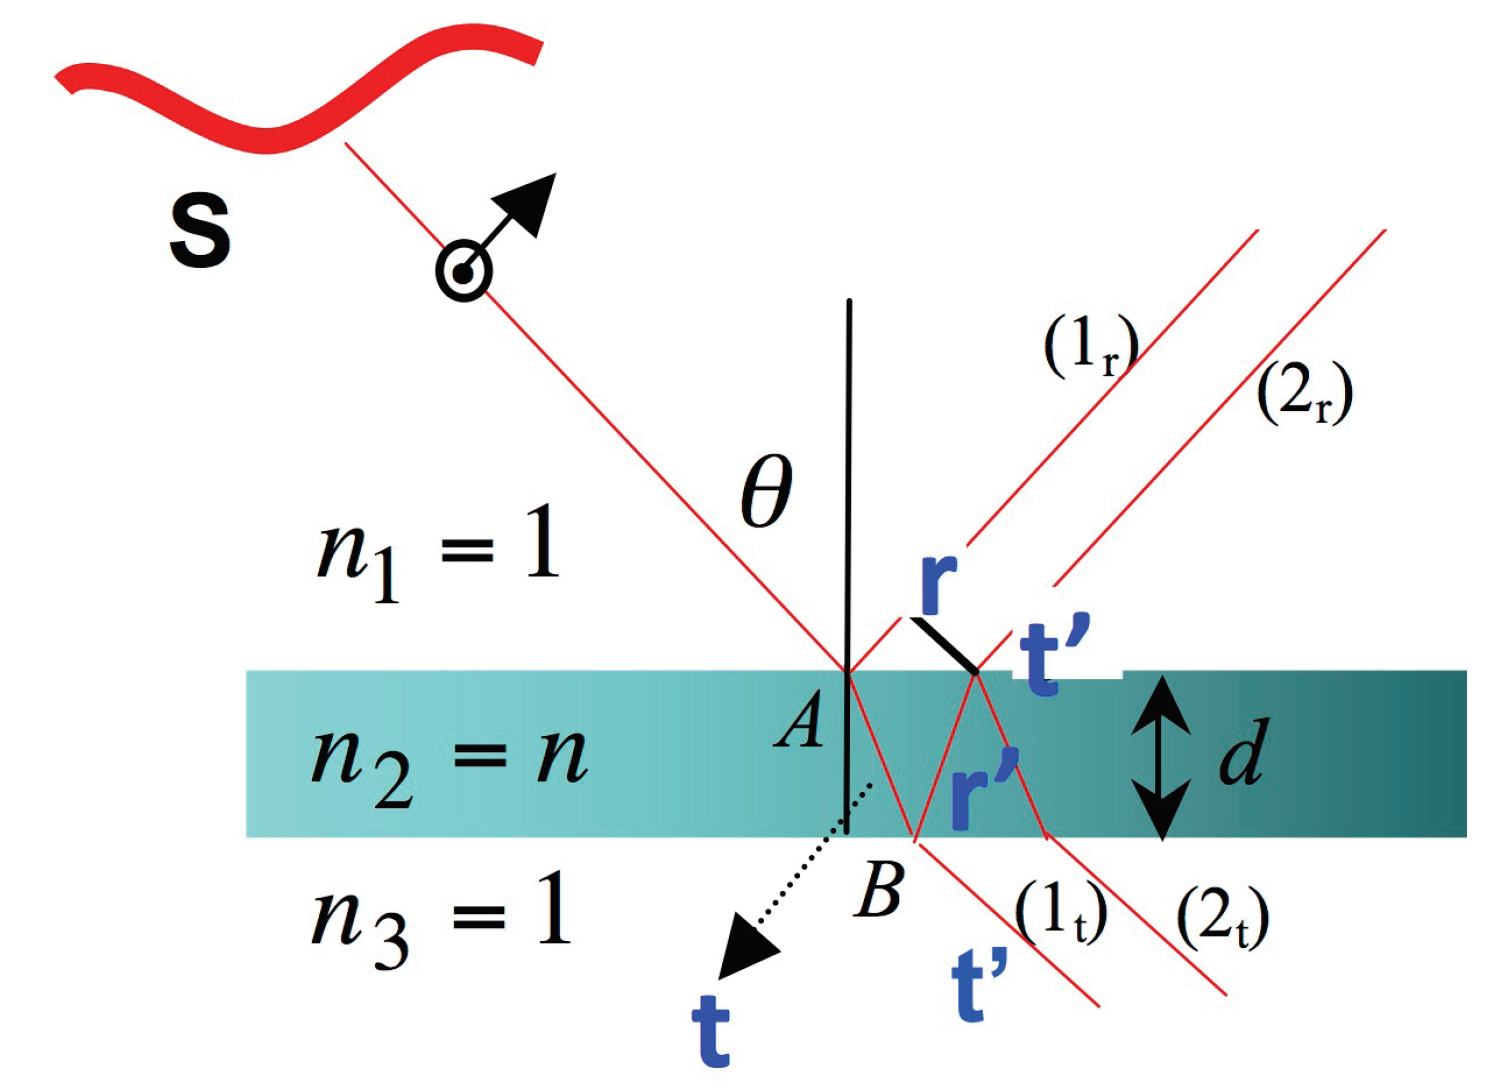
\includegraphics[scale=0.4]{03-Division_simple.png}
\caption{división simple de ondas con una lámina plana.}
\label{Fig:03.1-01}
\end{figure}

Esta luz reflejada (que no es mas que copias del campo inicial) se recogerán en usando una lente focal $f$, y se observarán en el plano focal. Usamos una lente focal por que nosotros queremos estudiar el patrón generado por la interferencia de la primera y segunda onda reflejada. Sin embargo estas, al ser paralelas, realmente nunca van a llegar a interferir. Colocar una lente focal hace que los dos rayos de luz converjan al mismo punto del plano focal de la lente. \\

Lo que queremos hacer ahora es calcular como es la forma del patrón de interferencia formado por ambos rayos. El estudio requiere calcular las intensidades $I_{r1}$ e $I_{r2}$, así como la diferencia de camino óptico en forma de fase $\Phi (x,y,z)$, tal que

\begin{equation}
I_{rT} (x,y,z) = I_{r1}+I_{r2} + 2 \sqrt{I_{r1} I_{r2}} \cos (\Phi(x,y,z))
\end{equation}
La pregunta que nos hacemos ahora: ¿Qué términos estan incluidos en la fase $\Phi$? La respuesta es bien sencilla: la diferencia de camino óptico, y la fase producida por la reflexión/trasmisión de la onda repetidas veces. Tal y como se puede ver en la figura \ref{Fig:03.1-02} tendremos que la diferencia de camino óptico viene dada por $k_0(\mathcal{L}_2 - \mathcal{L_1}) =k_0( n\cdot ABC-AD)$, y dado que $r'=-r$, la diferencia de fase producida por la reflexión-trasmisión es $\pm \pi$. Ahora bien, tenemos que evaluar todavía $ABC$ y $AD$ en distancias que conozcamos. Dado que el ángulo de reflexión es el mismo que el de incidencia, tenemos que $ {AD} = \sin(\theta) {AC}$, y si $AC=2  d \tan (\theta_t)$. Ahora nos queda por hallar $ABC$. En este caso $ABC=2AB$, donde $AB=d/\cos(\theta_t)$.

\begin{equation}
\Phi = k_0 \ccorchetes{\frac{2nd}{\cos (\theta_t)} - (2d\tan(\theta_t))\sin (\theta)}\pm \pi
\end{equation}
El ángulo $\theta_t$ se puede hallar por la ley de Snell $\sin (\theta) = n \sin (\theta_t)$. Si aplicamos esto a la ecuación anterior (y usando la relación $\cos^2 (\theta_t)= 1-\sin^2(\theta_t)$) obtenemos:

\begin{equation}
\Phi=k_0 2 n d \cos (\theta_t) \pm \pi
\end{equation}

\begin{figure}[h!] \centering
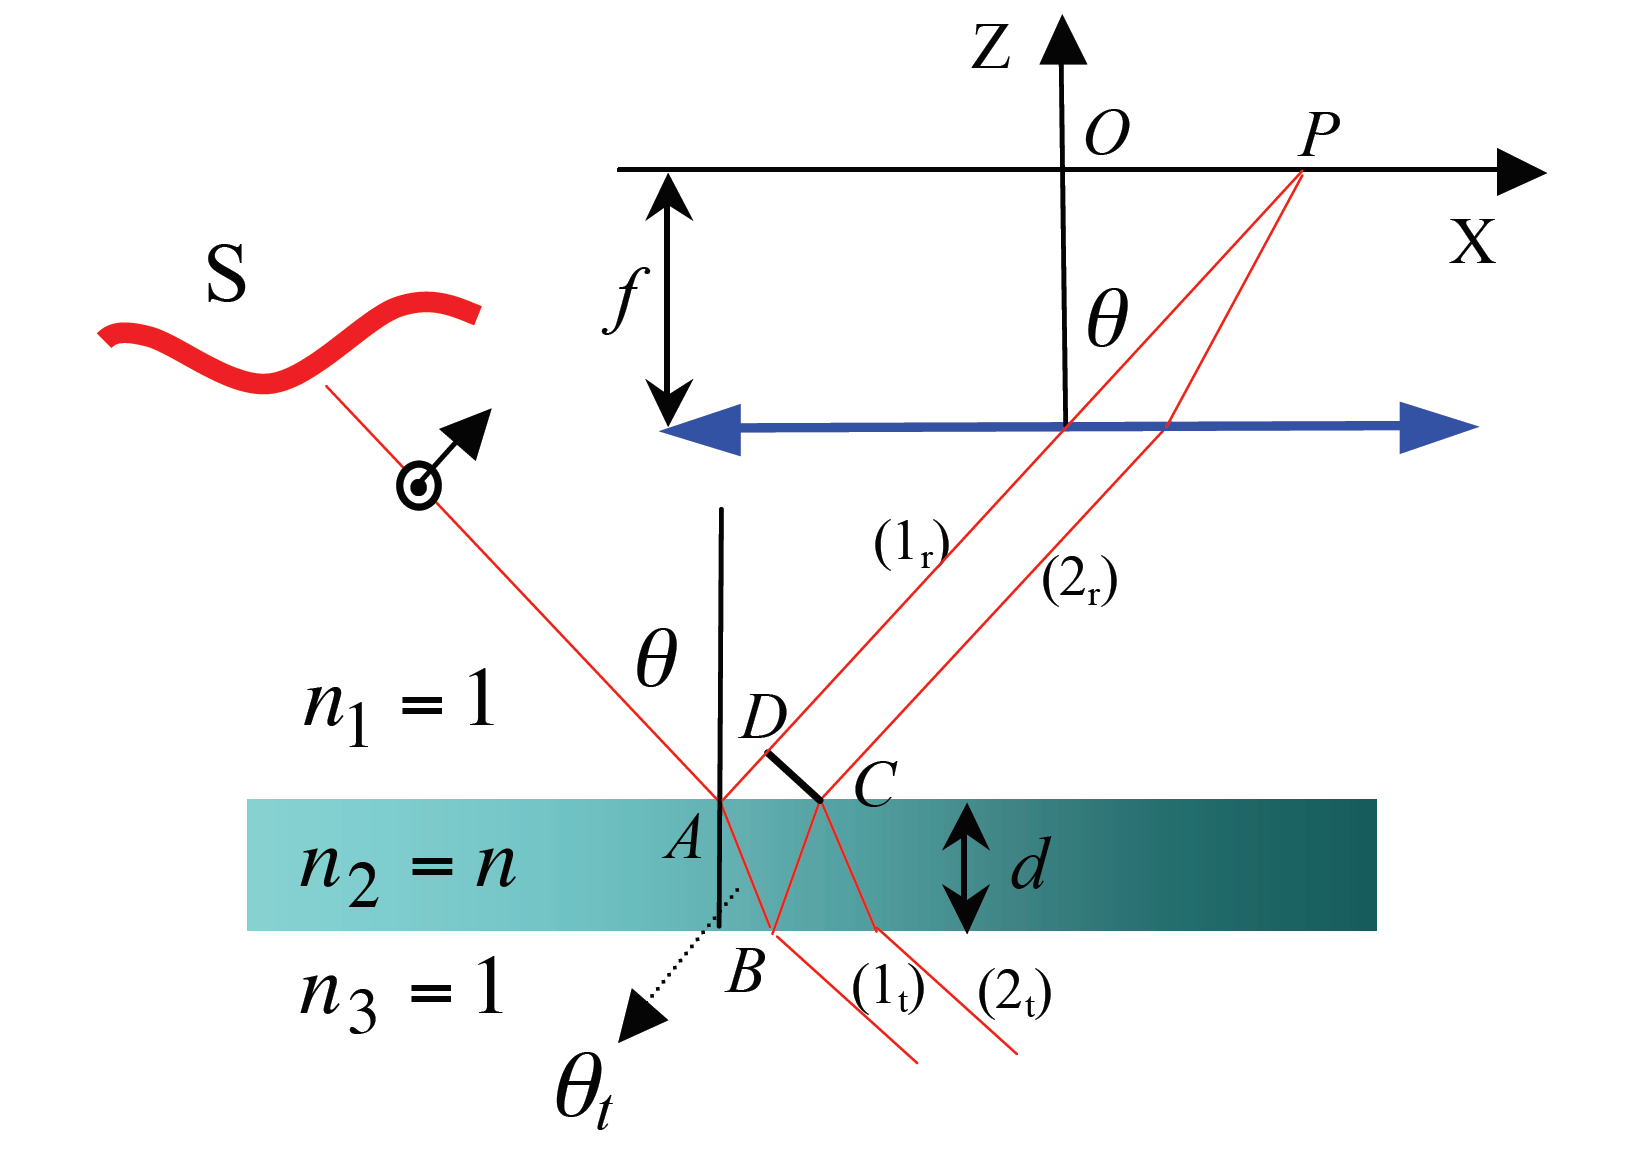
\includegraphics[scale=0.4]{03-Division_simple-2.png}
\caption{división simple de ondas con una lámina plana.}
\label{Fig:03.1-02}
\end{figure}

Ahora podemos darnos cuenta de una cosa: la incoherencia espacial \textit{no} es relevante. ¿Por qué? Porque todo rayo de luz procedente de cualquier otra posición con el mismo ángulo interfiere destructivamente, por lo que no es relevante. Si por ejemplo $n_3$ tuviera otro índice de refracción tendríamos que el factor $\pm \pi$ desaparecería. \\

Una vez tenemos el valor de $\Phi (\theta)$ podemos analizar el patrón obtenido en el plano focal. Supongamos que $I_{r1}\approx I_{r2} = I_{or}$, de tal modo que $\mathcal{V}_r \approx 1$. El patrón vendrá dado entonces por:

\begin{equation}
I_{rT} \approx 2I_{or} \ccorchetes{1-\cos \parentesis{2k_0 n d (n^2-\sin^2(\theta))^{1/2}}} \label{Ec:03.1-4}
\end{equation}
el factor menos que acompaña al coseno viene determiando por el factor $\pm \pi$. Dado que la intensidad $I_{rT}$ es constante cuando $\Phi$ es constante, siendo este último constante para un $\theta$ (o $\theta_t$) dado. Ahora bien, ¿Cómo se ve dicho patrón tras la focal? Aunque sorprenda, para cada ángulo en el plano focal se verá un anillo o franja circular de radio $\rho$ tal que $\rho =  f \tan (\theta)$. ¿Por qué? Pensemos en todos los rayos que inciden en el punto $A$ pero con un ángulo $\theta$. Tenemos que forman un círculo. Cada uno de estos tendrá su representación en el plano focal, pero no exactamente en el mismo punto, si no que formarán un círculo en el plano focal. Lógicamente el punto $P$ (tal y como se puede ver en la figura \ref{Fig:03.1-02}) estará a una distancia $\rho=f\tan(\theta)$. Usando las propiedades trigonométricas \\

\begin{equation}
\sin (\theta) = \frac{\rho^2}{\rho^2 + f^2}
\end{equation}

% Aqui podemos poner una imagen aunque hay que hacerla de cero

Sin embargo todo esto tiene un problema: que la lente exige una aproximación paraxial, por lo que el límite de la validez de las ecuaciones anteriores nos permiten describir los cosenos y senos usando las aproximaciones a ángulo pequeño ($\theta<<1$). En ese caso tenemos que $\tan(\theta) \approx \sin (\theta) \approx \theta \approx \rho/f$, tal que $\theta_t = \theta/n$. Luego $\cos (\theta_t) = 1-\theta_t^2/2 = 1 - \rho^2 / 2 f^2 n^2$:

\begin{equation}
I_{r} (\rho) \approx 2 I_{or} \ccorchetes{1- \cos \parentesis{2k_0 n d \parentesis{1- \frac{\rho^2}{2 f^2 n^2}}}}
\end{equation}

De este modo podemos obtener los \textbf{máximos} y \textbf{mínimos} simplemente haciendo que $\Phi_{\max}=(2m+1)\pi$ y $\Phi_{\min}= (2m)\pi$ con $m\in \mathbb{N}$. Nótese que el máximo de mayor orden corresponde a aquel con $\rho=\theta=0$. Las franjas se encuentran o bien localizadas en el infinito o en el plano focal de la lente. A estas franjas se les llama \textbf{franjas de igual inclinación} o \textbf{franjas de Haidinger}. \\

Hagamos ahora el mismo estudio pero para ondas trasmitidas. Las ondas trasmitidas verifican, casi siempre que $I_{t1}>>I_{t2}$. Además como $I_{t1}=|tt'|^2I_o$ e $I_{t2} =|tr'^2t'|I_o$, tenemos que la fase $\pm \pi$ no aparece. Suponiendo que el camino óptico lo calculamos siguiendo el mismo proceso que para la onda reflejada tenemos:

\begin{equation}
I_{tT} \approx I_{t1} + I_{t2} + 2 \sqrt{I_{t1} I_{t2}} \ccorchetes{ \cos \parentesis{2 k_0 d \parentesis{n^2 - \sin^2 (\theta)}^{1/2}}}
\end{equation}
Se puede justificar desde un punto de vista experimental (esto es, calculando $t,t',r'...$) que los valores típicos de de $I_{t1}$ son mucho mayores que los de $I_{t2}$ (esto es $I_{t1}>>I_{t2}$). Sin embargo existe otro método mucho más efectivo para calcular las intensidades: la \textit{conservación de energía}. Si $I_o$ es la intensidad total, entonces la intensidad interferncial trasmitida $I_{tT}=I_o - I_{rT}$, tal que $I_{rT}$ viene dada por la ecuación \ref{Ec:03.1-4}. De esta forma tenemos que:

\begin{equation}
I_{tT} = I_o - 2 I_{or} \ccorchetes{1-\cos \parentesis{2k_0 n d \cos\theta_t}}
\end{equation}
por lo que en la forma normal:

\begin{equation}
I_{tT} \approx (I_o - 2 I_{or})\ccorchetes{1+ \frac{2I_{or}}{I_o - 2 I_{or}} \cos \parentesis{2k_0 d \cos \theta_t}}
\end{equation}
Lógicamente si la fuente fuera policromática los padrones siguen siendo circulares aunque ahora tendrá colores. La interferencia siempre sucederá cuando se verifique la relación de coherencia $\tau = (2nd/c)<t_0$ siendo $t_0$ la duración de cada pulso. \\

Tanto para la reflexión como para la trasmisión las aberraciones ópticas para las lineas de luz no paraxiales, el tamaño finito de la lente hace que las interferencias pierdan visibilidad y acaben desapareciendo para un radio $\rho$ lo suficientemente grande.  

\subsection{Estudio ondulatorio paraxial de la interferencia}

Como hemos visto el estudio anterior suponía una onda perfectamente plana, proveniente de un objeto en el infinito. A partir del desarrollo anterior trataremos construir, la igual que antes, la forma de la intensidad interferencial, pero para ondas paraxiales. Al igual que antes, primero debemos hallar las expresiones paraxiales de la primera y segunda onda reflejadas de una lámina plano-paralela de espesor $d$ e índice $n$ en el vacío, iluminada por un punto que se encuentra en $(u,v,L)$. Comenzamos escribiendo la onda incidente:

\begin{equation}
\Encal_i (\rn) = \frac{-A_o' e^{-ik_0z}}{z-L} e^{i \frac{(x-u)^2+(y-v)^2}{2(z-L)}} \un
\end{equation}
donde $A_o'$ es un número complejo formado por $A_o' =A_o e^{ik_0L}e^{i \gamma}$ donde $A_o$ es un número real y $\gamma$ una fase aleatoria. Podemos ver que esta onda va de izquierda a derecha $| \ | \leftarrow$. Es interesante usar el siguiente código: $| \ | \rightarrow$ para la onda reflejada, $| \leftarrow | $ para la onda trasmitida, $|\leftrightarrow |$ para la onda que vuelve tras la segunda reflexión, y $|\leftrightarrow |\rightarrow$ para la segunda reflejada. A lo largo de este apartado (al igual que en el anterior) usaremos $r_1=r$, $t_1=t$, $r_2=r'$ y $t_2=t'$. \\

Calculemos pues la primera onda reflejada ($| \ |\rightarrow$). Tenemos que la primera onda reflejada debe venir dada por la continuidad de fases/amplitud, por lo que:

\begin{equation}
\Encal_{r1} = rA_o' \frac{e^{ik_0z}}{z+L} e^{i k_o0 \frac{(x-u)^2+(y-v)^2}{2(z+L)}} \un
\end{equation}

Calculemos ahora la primera onda trasmitida ($| \leftarrow |$). La ecuación tendrá que tener en cuenta que ahora la onda se mueve por el medio de índice de refracción $n$:

\begin{equation}
\Encal_{t1} = tA_o' \frac{e^{-ink_0z}}{z-nL} e^{-i n k_0 \frac{(x-u)^2+(y-v)^2}{2(z-nL)}} \un
\end{equation}

La segunda onda trasmitida ($|\leftrightarrow|$) deberá tener en cuenta que ha recorrida una distancia $d$. En ese caso tendremos que $r'=-r$: 

\begin{equation}
\Encal_{t2} = t(-r)A_o' \frac{e^{ink_0z}e^{ink_0d}}{z+nL+d} e^{-i n k_0  \frac{(x-u)^2+(y-v)^2}{2(z+nL+d)}} \un
\end{equation}
Ahora, la segunda onda reflejada ($|\leftrightarrow|\rightarrow$) vendrá dada por:

\begin{equation}
\Encal_{r2} = (-r)tt' A_o' \frac{e^{ik_0z}e^{ink_02d}}{z+L+2d/n}  e^{ik_0\frac{(x-u)^2+(y-v)^2}{2(z+L+2d/n)}} \un
\end{equation}

\subsection{Interferencia de ondas reflejadas}

Sea una fuente extensa con $\omega=k_0 c$ iluminando por reflexión un divisor de haces de luz. Un \textbf{divisor de haces de luz} es generalmente una lámina plano paralela fina con un coeficiente de \textit{reflectancia} $R=1/2$ (y por tanto la \textit{trasmictancia} $T=1/2$), rotada $\pi/4$, tal y como se muestra en la figura \ref{Fig:03.1-03} La onda reflejada, al ``rebotar'' irá hacia la lámina plano paralela , de tal modo que se formará una onda reflejada 1 y otra onda reflejada 2 con menor amplitud. Para llegar a la lente deberá trasmitirse de nuevo a través del divisor de haces, por lo que la intensidad total se verá reducida 1/4 , o lo que es lo mismo, la amplitud del campo se verá reducida en 1/2. 

\begin{figure}[h!] \centering
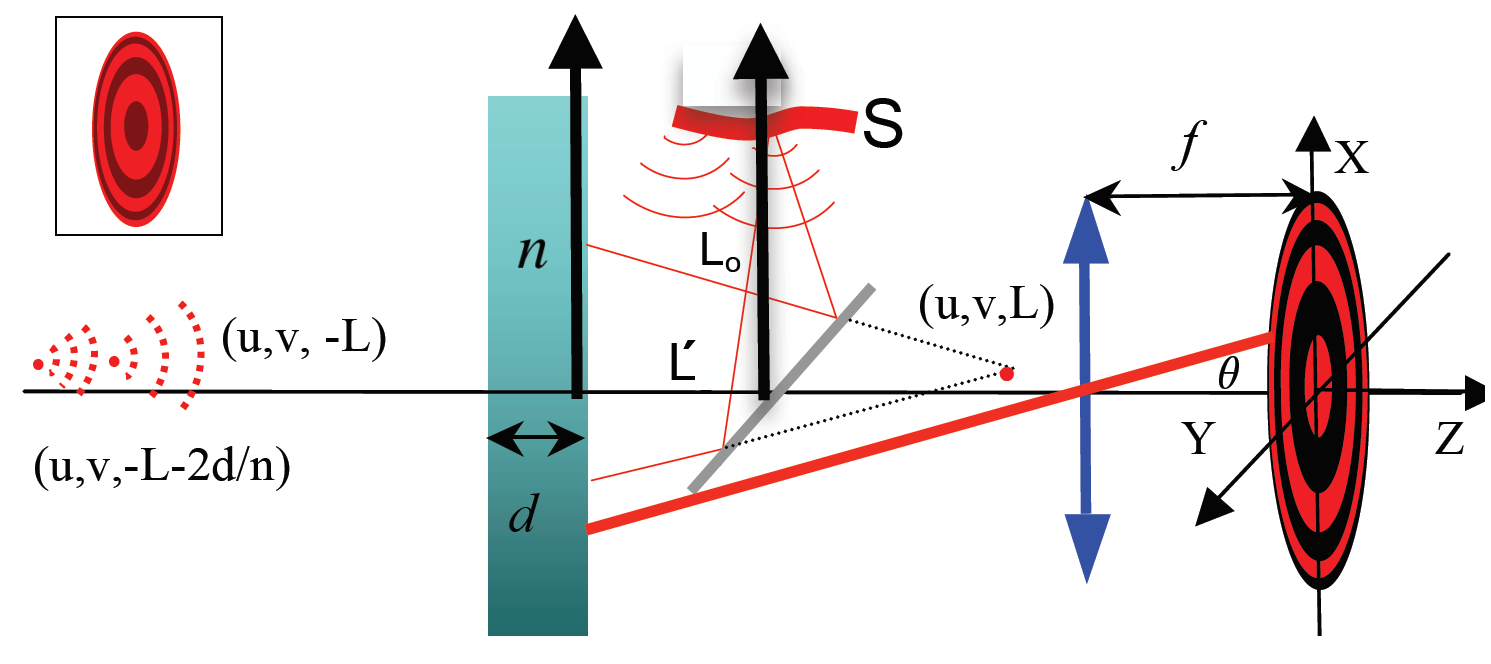
\includegraphics[scale=0.4]{03-Division_simple-3.png}
\caption{}
\label{Fig:03.1-03}
\end{figure}

Debido a la relfexión de la onda en el divisor tendremos que la fuente ubicada en $(L_0,v,u)$ parecerá que viene del $(u,v,L_0)$. Como ya hemos estudiado, los campos vendrán dado por las expresiones anteriores salvo un factor $1/2 $:

\begin{equation}
\Encal_{r2} = (-r)tt' A_o' \frac{1}{2} \frac{e^{ik_0z}e^{ink_02d}}{z+L+2d/n}  e^{ik_0\frac{(x-u)^2+(y-v)^2}{2(z+L+2d/n)}} \un
\end{equation}
\begin{equation}
\Encal_{r1} = rA_o'  \frac{1}{2} \frac{e^{ik_0z}}{z+L} e^{i k_0 \frac{(x-u)^2+(y-v)^2}{2(z+L)}} \un
\end{equation}
Lo que ocurrirá en este caso es que la onda parecerá que viene de dos puntos diferentes, por el simple hecho de que uno atravesó (y regresó) la lámina. Es de una importancia capital decir que tanto los campos TE como los campos TM reflejados son los mismos, salgo por un signo de $r$. En cualquier caso diferenciarse por una fase global $\pi$ es irrelevante. Si consideramos las aproximaciones $tt' \approx 1$ y $2d/n <<L$ tenemos que:

\begin{equation}
I_r(\rn) \approx \frac{R}{2} \frac{|A_o (u,v)|^2}{(z+L)^2} \ccorchetes{1- \cos \parentesis{nk_o 2d \parentesis{1-\frac{(x-u)^2+(y-v)^2}{2n^2(z+L)^2}}}}
\end{equation}
siendo $R=|r|^2$. De nuevo el signo menos procede del factor negativo $r'=-r$. Si $n_3>n_2>n_1$ este factor desaparecería, y el coseno iría con un + delante. Ahora lo único que queda hacer es el análisis de la intensidad interferencial, esto es, analizar como es el patrón, que forma tiene, y ver cuando ocurren los máximos y los mínimo. Sea, por simplicidad, $nk_0 2 d=\pi(2p+1)$ con $p \in \mathbb{N}$. Si $\tilde{x}=(x-u)$ y $\tilde{y}=(y-v)$ tenemos que para que haya un \textit{máximo}

\begin{equation}
(2p+1)\pi - (2p+1)\pi \frac{\tilde{x}^2 + \tilde{y}^2}{2n^2(z+L)^2} = (2m+1)\pi \Rightarrow \frac{\tilde{x}^2 + \tilde{y}^2}{2n^2(z+L)^2} = \frac{2(p-m)}{(2p+1)}
\end{equation}
y para que haya un \textit{mínimo}:
\begin{equation}
(2p+1)\pi - (2p+1)\pi \frac{\tilde{x}^2 + \tilde{y}^2}{2n^2(z+L)^2} = 2m\pi \Rightarrow \frac{\tilde{x}^2 + \tilde{y}^2}{2n^2(z+L)^2} = \frac{2p-2m+1}{2p+1}
\end{equation}
Como podemos ver, para una superficie, tenemos que $p\in\mathbb{N}$ es un \textit{número fijo}, que no varía. Para que el radio sea positivo debe verificarse que $m\leq p$, por lo que en realidad tendremos un número límitado de franjas de máximos y mínimo. El máximo central ocurrirá cuando $m=p$, y el mínimo mas cercano ocurre también cuando $m=p$. Recordemos que antes hemos definido $(2p+1)=nk_02d/\pi$. El siguiente máximo/mínimo será cuando $m=p-1$... Si nos centramos en el primer mínimo, este tendrá un radio ($\rho_c^2=\tilde{x}^2+\tilde{y}^2$) de

\begin{equation}
\rho_c^2 = \frac{2n^2(z+L)^2}{2p+1} = \frac{ \pi n}{k_0d} (z+L)^2
\end{equation}
Como podemos comprobar la anchura del disco central aumenta con la distancia de propagación $z$.  Si $z\rightarrow\infty$ tenemos que $\Phi$ deja de depender de $x$ e $y$, tal que $\Phi=2k_0 nd$. En este caso también deja de depender de $u$ y $v$, por lo que en este caso el tamaño radial del disco central sería tan grande que un desplazamiento en ($u,v$) es despreciable. Es decir, cuando $z\rightarrow\infty$ tenemos que la incoherencia espacial se elimina, ya que da igual el punto ($u,v$), que se generará el mismo patrón interferencial.

\subsection{Interferencia con una fuente extensa}
 
Como hemos dicho antes la incoherencia espacial desaparece cuando $z\rightarrow\infty$. Una forma de implementar el infinito sin tener que llevar el patrón al infinito es usar una lente. En el plano focal de una lente se implementa el infinito, con patrones interferenciales finitos, y con todos los patrones coincidentes. En ese caso tenemos que $z+L \rightarrow f$ y $u=v=0$. Esto último es porque, al implementar el infinito usando la lente, tenemos que la posición $(u,v)$ del punto de luz no importa, solo importa el punto $(x,y)$ del patrón. Entonces la intensidad interferncial:
 
\begin{equation}
I_r(\rn) \approx \frac{R}{2} \frac{|A_o (u,v)|^2}{f^2} \ccorchetes{1- \cos \parentesis{nk_o 2d \parentesis{1-\frac{x^2+y^2}{2n^2f^2}}}}
\end{equation}
Si ahora quisiéramos hallar la interferencia obtenida con una fuente extensa, con un continuo de patrones interferenciales desplazados, tendríamos que implementar una lente focal para evitar que $I_{rT} \approx cte$. De implementarla el patrón obtenido es:

\begin{equation}
I_{rT} (x,y,z) \approx \frac{R}{2f^2} \ccorchetes{1- \cos \parentesis{nk_o 2d \parentesis{1-\frac{x^2+y^2}{2n^2f^2}}}}\int |A_0 (u,v)|^2 \D u \D v 
\end{equation}
donde $I_{or} = \frac{R}{2f^2} \int |A_o(u,v)|^2 \D u \D v$. Si usamos la relación $\theta=\rho/f$, usando la aproximación a ángulo pequeño $\cos(\theta_t) = 1 - \theta^2/2n^2$, tenemos que:

\begin{equation}
I_{rT}(x,y,z) \approx 2 I_{or}(1-\cos (2k_0 n d \cos\theta_t))
\end{equation}
lo cual concuerda con la división simple de amplitud en su aproximación casi-ondulatoria, ya que implementar el infinito es como suponer que los puntos luminosos generan ondas planas. 

\section{Interferencia en láminas de espesor variable}

\subsection{Interferencia por reflexión}

Una lámina de espesor variable con función de espesor $d(\rn)$ producirá, bajo ciertas condiciones, interferencia por división de simple de amplitud. Es de interés introducir la función de espesor $d(\rn)$ como la diferencia entre dos superficies 

\begin{equation}
d(\rn)=[d_0 +z_{(2)}(x,y)]-z_{(1)} (x,y)
\end{equation}
Para hallar y analizar ondulatoriamente la interferencia de estas láminas de espesor variable usamos las funciones de trasmisión variable y reflexión, bajo incidencia progresiva de una superficie $z(x,y)$ separando dos medios de índices $n_1$ y $n_2$:

\begin{equation}
t(x,y) = t e^{ik_0 (n_1-n_2) z(x,y)} \tquad r(x,y) = re^{ik_0 2 n_1 z(x,y)}
\end{equation}
Lógicamente la primera discontinuidad verificará que $z_{(1)}=0$ en el plano de referencia $z=0$ y la segunda discontinuidad verificará que $z_{(2)}=0$ en el plano de referencia $d_0$. Uno de los grandes problemas de las láminas de espesor variable es que permiten calcular el patrón interferencial únicamente en las proximidades de la lámina, esto en $z\approx 0$. Por esa misma razón podemos suponer que:

\begin{equation}
\Ecal_{r1} = r e^{ik_0 z_{(1)}(\rn)} \Ecal_i
\end{equation}
\begin{equation}
\Ecal_{r2} = (-r)tt' e^{ik_0n_2z_{(2)}}e^{i2k_0d}e^{-i2k_0(n_2-1)z_{(1)}} \Ecal_i
\end{equation}
donde el $2k_k(n_2-1)z_{(1)}$ viene de la trasmisión dos veces seguidas. En uno va de $n\rightarrow 1$, y en otro de $1 \rightarrow n$, por lo que deberían cancelarse, pero es la superficie que pasa de $z_{(1)} \rightarrow - z_{(1)}$ la que hace que se sumen. Supongamos que $I_0=|\mathcal{E}_i|^2$ (intensidad reducida), siendo $R=|r|^2=|r'|^2$. En ese caso el patrón de intensidades $I_{rT}$ podemos obtenerlo fácilmente

\begin{equation}
I_{rT} = 2R I_0 \ccorchetes{1-\cos( 2k_0n(z_{(2)}(\rn)+d_0-z_{(1)})} = 2 R I_0 \ccorchetes{1-\cos (2k_0nd(\rn)}
\end{equation}

Como podemos ver el patrón ($\Phi$) es independiente del punto $(u,v)$ de la fuente. La única dependencia con $(u,v)$ viene dada por $|\Ecal (u,v)|^2$. Al ser emisores puntuales e incoherentes podemos sumar todos los patrones, de tal modo que:

\begin{equation}
I_{or} = \int \frac{|A_o (u,v)|^2 R}{L^2} \D u \D v
\end{equation}
y así la \textbf{intensidad total reflejada} para una \textit{fuente extensa} toma la forma:

\begin{equation}
I_{rT} = I_{or} \ccorchetes{1-\cos (2k_0nd(\rn)}
\end{equation}
De aquí podemos extraer importantes conclusiones, tales como:

\begin{itemize}
\item La interferencia está localizada en las proximidades de la lámina $z\approx0$. En este caso todos los puntos de la fuente $(u,v)$ producen la misma interferencia. \\
\item La intensidad interferencial producida por una lámina e espesor variable (LEV) delgada con una fuente extensa puede usarse para hallar la función de espesor $d(\rn)$. 
\end{itemize}
Siempre que nos alejemos de la lámina, las ondas obtendrán expresiones complicadas y cuya forma dependerá ademas del punto de la fuente ($\Ecal_{r1}(x,y,z,u,v,),\Ecal_{r2}(x,y,z,u,v,)$). Además los patrones interferenciales estarán desplazados, e incluso llegarán a ser diferentes. Es decir $I_{rT} = cte$. \\

En este caso las ecuaciones de los máximos y mínimos que definen las complejas curvas de igual $I_{rT}$, las llamadas \textbf{franjas de igual espesor} o \textbf{franjas de Fizeau} vienen dadas por:

\begin{equation}
2nd (\rn_{\max}) = (m+1/2)\lambda_0 \tquad 2nd(\rn_{\min}) = m \lambda_0
\end{equation}
En el caso de una \textit{fuente policromática} tendremos que la itennsidad total tendrá forma de:

\begin{equation}
I_{rT} \approx \int I_{or} \ccorchetes{1-\cos (2k_0nd(\rn)} \D \omega
\end{equation}

\subsection{Interferencia por trasmisión}

La interferencia por trasmisión viene dada por:

\begin{equation}
I_{tT} = (I_o - 2I_{or}) \ccorchetes{1- \frac{2I_{or}}{(I_o-2I_{or})}\cos (2k_0nd(\rn))}
\end{equation}


\section{Interferómetro de Michelson y aplicaciones}

\begin{figure}[h!] \centering
\includegraphics[scale=0.27]{Interferometro_michelson.pdf}
\caption{interferómetro de Michelson.}
\label{Fig:03.3-01}
\end{figure}


Un \textbf{interferómetro de Michelson} (IM) es un dispositivo consituido por dos espejos que denotaremos por $\mathsf{E}_1$ y $\mathsf{E}_2$; y un divisor de haz con $R=T=1/2$. Los espejos se disponen perpendicularmente de tal manera que el divisor de haces forme un ángulo de $\pi/4$ con los espejos. Las fases del camino óptico pueden cancelarse con una lámina llamada la \textbf{lámina compensadora}. En la imagen \ref{Fig:03.3-01} podemos ver un interferómetro de Michelson.

\subsection{Estudio ondulatorio}

Sea un interferómetro de Michelson donde los puntos de la fuetne extensa casi-monocromática de frecuencia $\omega=k_0c$ se encuentran aproximadamente a una distancia $L_0$ del divisor de haces de luz, y los espejos a $L$ y $L+d$. Si consideramos una fuente luminosa en $(-L_0,v,-u)$ como el de la figura  \ref{Fig:03.3-02}, podemos ver que los puntos desde los cuales parece que parten los rayos de luz (tras pasar por el divisor y los espejos) son $(u,v,-L_0-2L')$ para el rayo de luz que se refleja en $\mathsf{E}_1$ y $(u,v,-L-2L'-2d)$ para el que se refleja en $\mathsf{E}_2$. Si llamamos a $L=L_0+2L'$, obtenemos directamente las siguientes expresiones:

\begin{equation}
\Encal_1(x,y,z) = \frac{1}{2} \frac{e^{i\pi} A_0(u,v)}{(z+L)} e^{ik_0 (z+L)} e^{ik_0 \frac{\tilde{x}^2+\tilde{y}^2}{2(z+L)}} \un
\end{equation}
\begin{equation}
\Encal_2(x,y,z) = \frac{1}{2} \frac{e^{i\pi} A_0(u,v)}{(z+L+2d)} e^{ik_0 (z+L+2d)} e^{ik_0 \frac{\tilde{x}^2+\tilde{y}^2}{2(z+L+2d)}} e^{i\pi} \un
\end{equation}
por lo que obtenemos la siguiente intensidad interferencial por la salida vertical:

\begin{equation}
I(x,y,z) \approx \frac{|A_o(u,v)|^2}{2(z+L)^2} \ccorchetes{1- \cos \parentesis{2k_0d \parentesis{1-\frac{\tilde{x}^2+\tilde{y}^2}{2(z+L)^2}}}}
\label{Ec:03.3-36}
\end{equation}
Obtenemos así \textbf{franjas circulares} cuyo centro depende de $(u,v)$ y  cuyo tamaño crece a medida que nos alejamos del plano $z$ de observación. Desde este punto el interferómetro de Michelson opera como una lámina ficticia de índice $1$ y espesor $d$. 


\begin{figure}[h!] \centering
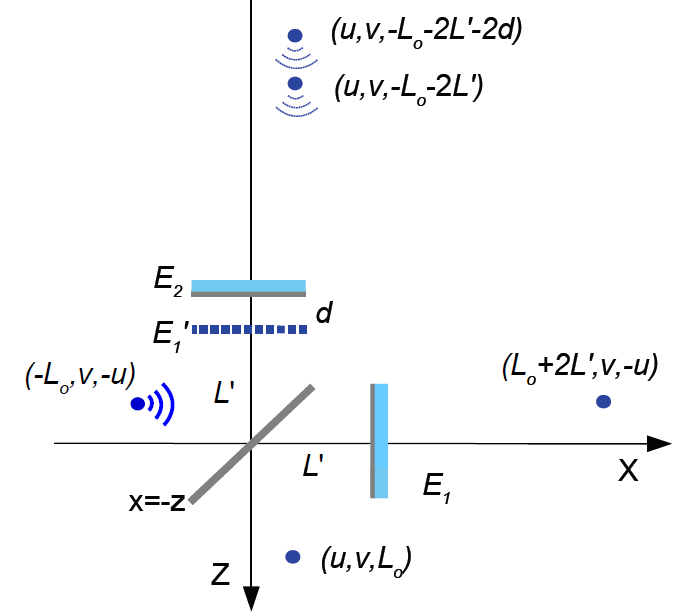
\includegraphics[scale=0.7]{03-Division_simple-4.png}
\caption{interferómetro de Michelson.}
\label{Fig:03.3-02}
\end{figure}

\subsection{Fuente extensa}

Igual que en el caso de las láminas paralelas, si la fuente es especialmente incohernete entonces en cualquier plano de observación tendremos una superposición continua de patrones interferenciales con distribuciones de intensidad dadas por la ecuación \ref{Ec:03.3-36}. Para fuentes suficientemente extensas la intensidad en dichos planos será casi-uniforme expcepto en el infinito. Como el infinito es, en la práctica, inalcanzable, la única manera de implementarlo es usar una focal convergente, de tal modo que da igual el punto de la fuente, se generará el mismo patrón. Entonces los cambios $(u,v)\rightarrow(0,0)$ y $(z+L)=f$ nos llevan a que:

\begin{equation}
I_{vT}  = \frac{I_{ov}}{2} \ccorchetes{1-\cos \parentesis{2k_0 d \parentesis{1-\frac{x^2+y^2}{2f^2}}}}
\end{equation}
tal que si usamos la típica expresión $\theta=\sqrt{x^2+y^2}/f = \rho/f$ obtenemos ahora si


\begin{equation}
I_{vT}  = \frac{I_{ov}}{2} \ccorchetes{1-\cos  2k_0 d \cos \theta}
\end{equation}

\subsection{Aplicaciones en Metrología}

Una de las aplicaciones mas interesantes de el interferómetro de Michelson es su aplicación en la metrología. La metrología es la ciencia de las mediciones, estudiando tanto la medida como su incertidumbre. Veamos algunas de estas. \\

Uno de ellos es la \textbf{medida de pequeños espesores} o \textbf{índices de refracción}. Supongamos que inicialmente el interferómetro de Michelson lo tenemos en camino nulo ($d=0$). En este caso obtendremos un campo casi uniforme. Posteriormente introducimos una lámina delgada de espesor $e$. En ese caso aparecerán una serie de anillos, provenientes de la fase interferencial adicional $\Phi = k_0 (n-1)(2e)$. Luego necesitamos desplazar $\Delta D$ el espejo $E_1$ para así compensar el camino óptico de la lámina. Si $\Delta'=2(n-1)e=2\Delta d$ con $2\Delta d = \Delta m \lambda_0$ siendo $\Delta m$ el número de anillos, tendremos que podremos calcular $e$ como

\begin{equation}
e = \frac{\Delta m \lambda_0}{2(n-1)} \tquad n=1+\dfrac{\Delta m \lambda_0}{2e}
\end{equation}

Otra de las aplicaciones metrológicas mas útiles es la inspección de superficies ópticas de \textbf{Twyman-Green}. Diremos que el elemento óptico bajo prueba es de una alta calidad siempre que el patrón interferencial obtenido usando esta variante de Michelson sean líneas rectas. Si las líneas no son rectas, mostrando ciertas desviaciones de las mismas, podremos suponer que la lente no es una lente perfecta y por tanto habrá que corregirla. Además muestra la imperfección del elemento. 


\subsection{Aplicaciones en espectroscopia atómica: intensidad espectral}

Podemos medir la \textbf{intensidad espectral} $I(\omega)$ a partir de $I(x)$. Supongamos un interferómetro de Michelson con los espejos formando un pequeño ángulo $\sigma$ con fase inicial $\epsilon_F=\pi$. Entonces si $\Delta \Phi = 2k_0nx\sigma$, suponiendo $\omega = nk_0c$ obtenemos que:

\begin{equation}
I(x) = \int  \frac{I(\omega)}{2} \ccorchetes{1 - \cos \parentesis{\frac{2\omega x \sigma}{c}}} \D \omega
\end{equation}
Si definimos $\tau=2\sigma x/c$ y a $I(\tau) = [Q-4I(x) ]$ (siendo $Q=\int 2 I_0 \D \omega$, tenemos que la inversa de esta integral nos permite calcular:

\begin{equation}
I(\omega) = \int I(\tau) \cos (\omega \tau) \D  \tau
\end{equation}

\subsection{Aplicaciones en espectroscopia atómica: dobletes}

Otra de aplicación interesante es la medida de un \textbf{doblete atómico}, esto es, medir la separación energética $\Delta E = \hbar \Delta \omega$ entre dos niveles de energía muy cercanos entre sí; así como medir la separación cromática y las longitudes de onda de la emisión atómica (que es, al fin de al cabo, lo mismo). Para esto debemos usar el campo de visiblidad del patrón interferencial. Si una onda emite dos ondas, de frecuencia $\omega_{pm} = (\omega_c \pm \Delta \omega/2)$, tendremos que $k_{pm}=\omega_{pm}/c$; verificándose que $\Delta \omega << 1$, y que $I_+=I_-=I_0$, tenemos que:

\begin{equation}
I(x,y,z) = \frac{I_o}{2}  \ccorchetes{1+ \cos \parentesis{\frac{\Delta \omega_c d}{c} \cos (\theta)} \cos \parentesis{\frac{2d\omega_c}{c} \cos (\theta)}}
\end{equation}
Donde lógicamente podemos aplicar que $\Delta \omega d \cos \theta /c \approx \Delta \omega d/c$, dado que $\Delta \omega << 1$. Eso nos lleva a:


\begin{equation}
I(x,y,z) = \frac{I_o}{2}  \ccorchetes{1+ \cos \parentesis{\frac{\Delta \omega_c d}{c}} \cos \parentesis{\frac{2d\omega_c}{c} \cos (\theta)}}
\end{equation}
y por tanto a una visibilidad dependiente de $\Delta \omega$, tal que $\mathcal{V}= |\cos (\Delta \omega d /c)|$. Luego variando $d$ podemos obtener las llamadas \textbf{coincidencias interferenciales} $\Delta \omega d /c = N \pi$ o las llamadas \textbf{anticoincidencias interferenciales} $\Delta \omega d / c = (N+1/2) \pi$. Seleccionamos un patrón anticoincidente tal que $d_1=(N+1/2)\pi c /\Delta \omega$. Si movemos $d_2$ hasta la siguiente anticoincidencia $d_2 = (N+3/2)\pi c /\Delta \omega$, tendremos que:

\begin{equation}
\Delta d = \pi c/\Delta \Omega
\end{equation}
o lo que es lo mismo:

\begin{equation}
\Delta E = \hbar \Delta \omega = \hbar \frac{\pi c}{\Delta d}
\end{equation}

\subsection{Aplicaciones en relatividad: detección de ondas gravitacionales}

Uno de los detectores mas famosos de ondas gravitacionales, el LIGO (\textit{Laser Interferometer Gravitational-Wave Observatory}) consiste en un interferómetro de Michelson. Las principales características de este detector es que sus brazos son cavidades ópticas Fabry-Perot con una gran longitud. El fin de estas cavidades no es otro que aumentar la \textit{longitud efectiva} de los brazos por múltiples reflexiones internas de los brazos. \\

Las onda gravitacionales, en la aproximación lineal de la teoría de la relatividad general, son capaces de producir pequeños desplazamientos en la curvatura del espacio-tiempo que los rayos de luz sienten (ya que los espejos se desplazan un $\delta L$), alterando la fase de las ondas al recorrer mas o menos camino. Se puede probar que dicho desfase $\delta L$ viene determinado por la longitud del brazo del detector $L$ y la amplitud de la onda gravitacional $h$, tal que 

\begin{equation}
\delta L = \frac{hL}{2}
\end{equation}
Esto se prueba usando la métrica en el plano del interferómetro dada por las ecuaciones $c^2\D t^2 = (1+h)\D x^2 + (1-h) \D z^2$. En una onda gravitacional $h(t)$ depende del tiempo. Usemos entonces onda planas (láser) con una fase $\epsilon_F=\pi$ y una fase adicional $\epsilon_a=-\pi/2$ en el camino vertical. Si el camino en uno de los brazos se ve modificado tal que $x'=(1+h/2)x$ y $z'=(1-h/2)z$, tendremos que $L$, las ondas emergentes:

\begin{equation}
\Ecal_1 \approx \frac{E_0}{2} e^{i2k_0L_{x'}} e^{ik_0z'}
\end{equation}
\begin{equation}
\Ecal_2 \approx \frac{E_0}{2} e^{i2k_0 L_{z'}} e^{ik_0z'}
\end{equation}
por lo que $I(t)$ vendrá dado por:

\begin{equation}
I(t) = \frac{E_0^2}{2} \ccorchetes{1+ \cos \parentesis{\pi/2 - 2k_0 h(t)L}} \approx   \frac{E_0^2}{2} \ccorchetes{1 + 2k_0 h(t)L} 
\end{equation}
luego obtenemos que

\begin{equation}
h(t) = \frac{1}{2k_0 L} \ccorchetes{\frac{2I(t)}{I_0}-1} \tquad I_0 = E_0^2
\end{equation}



\section{Interferómetro de Match-Zehnder}
\subsection{Introducción}
El interferómetro de Match-Zehnder es, después del interferómetro de Michelson, uno de los sistemas interferómetricos más versátiles para el análisis de fenómenos interferenciales, tanto cuánticos como clásicos. Se componente, básicamente, de dos divisores de haces y dos espejos rotados $\pi/4$. En cada camino podemos interponer elementos ópticos, como láminas plano-paralelas, lentes... Estos elementos estan caracterizados por funciones de trasmisión del tipo:

\begin{equation}
t_{(h,v)}(x,y) = |t_{(h,v)} (x,y) | e^{i \Phi_{(h,v)} (x,y)}
\end{equation}

Además tendremos dos salidas con intensidades $I_h$  e $I_v$, que se evaluarán mediante los detectores $D_h$ y $D_v$ respectivamente. Es interesante distinguir entre varios tramos: $h_ov_o$ antes del primer divisor, $h_1v_1$ antes de los dos espejos, $h_1'v_1'$ después del primer pero antes de los posibles elementos ópticos, $h_2v_2$ después de los elementos ópticos y $hv$ después del segundo divisor de onda.

\begin{figure}[h!] \centering
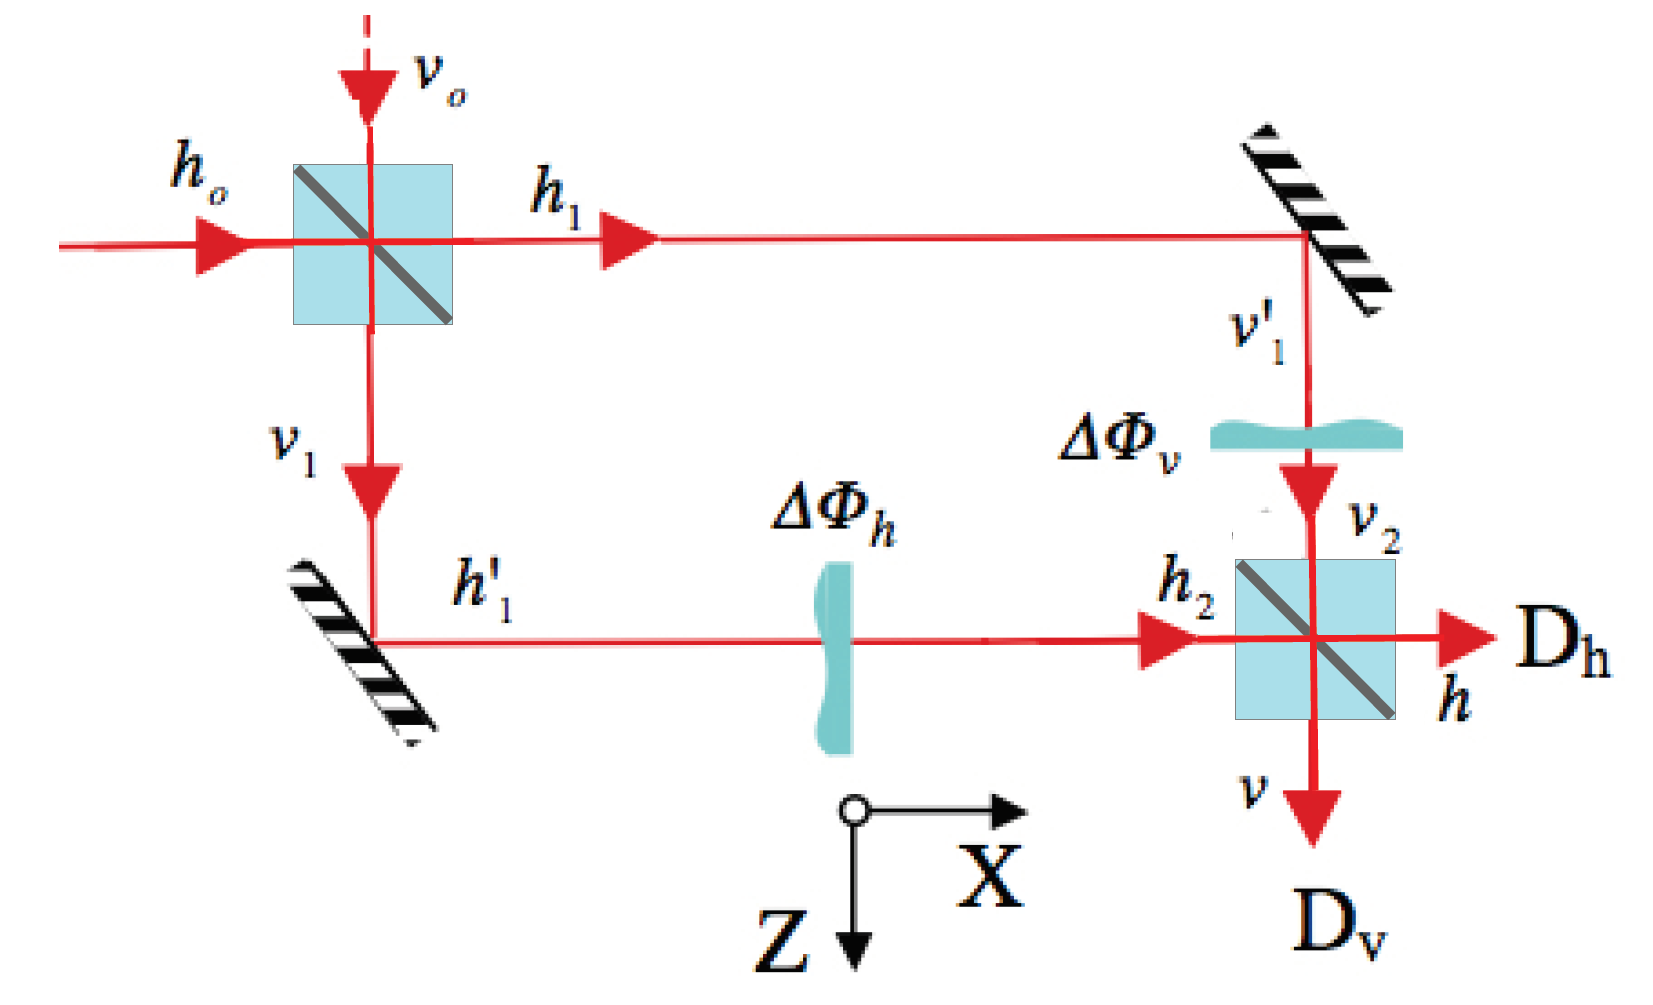
\includegraphics[scale=0.27]{03-Match_Zehnder.png}
\caption{interferómetro de Match-Zehnder.}
\label{Fig:03.4-01}
\end{figure}

En esta sección vamos a ir calculando los valores de los campos en una aproximación casi-ondulatoria:

\begin{itemize}
\item  \textbf{Primer divisor}: si suponemos que las ondas de luz son o TM o TE (para si solo considerar una trasmictancia $\mathcal{T}$ o reflectancia $\mathcal{R}$). Sin perdida de generalidad, usando la \textit{conservación de energía}, podemos suponer que:

\begin{equation}
\mathcal{E}_{h1} = \mathcal{T}^{1/2} \mathcal{E}_{ho} - \mathcal{R}^{1/2} \mathcal{E}_{vo} \tquad 
\mathcal{E}_{v1} = \mathcal{T}^{1/2} \mathcal{E}_{vo} + \mathcal{R}^{1/2} \mathcal{E}_{ho}
\end{equation}
Aunque, en general, el cambio mas general posible es aquel que hace que se verifique $|\mathcal{E}_{h1}|^2+|\mathcal{E}_{v1}|^2=|\mathcal{E}_{ho}|^2+|\mathcal{E}_{vo}|^2$, tal y como pueden ser $ mathcal{E}_{h1} = \mathcal{T}^{1/2} + i \mathcal{E}_{ho} - \mathcal{R}^{1/2} \mathcal{E}_{vo}$ p $ \mathcal{E}_{v1} = i \mathcal{T}^{1/2} \mathcal{E}_{vo} + \mathcal{R}^{1/2} \mathcal{E}_{ho} $.

\item \textbf{Espejos}: por otra banda los espejos introducen una fase de salto $\pi$ y la trasnformación permutativa $h \leftrightarrow v$. Esto es, la onda vertical pasa a ser la horizontal y viceversa. Esto es implementable (al igual que lo anterior) mediante matrices, al igual que en  los polarizadores. 

\item \textbf{Elementos de fase:} las trasformaciones de fase producidas por los elementos ópticos delgados justo después de los espejos (en nuestro esquema). En ese caso tenemos que: 

\begin{equation}
\Ecal_{(h_2,v_2)} = \ccorchetes{t e^{i\Phi_{(h,v)}} e^{-ik_0d}} \Ecal_{(h_1',v_1')} \approx e^{i\Delta\Phi_{(h,v)}} \Ecal_{(v_1',h_1')}
\end{equation}

\item \textbf{Segundo dividor}: finalmente a la salida tenemos un nuevo divisor de haces entre los campos de entrada y los de salida. Podemos coger la misma ecuación que cogimos para el primer divisor.
\end{itemize}

\subsection{Interferencia con ondas planas}

Consideremos un divisor típico con $\mathcal{R}^{1/2}=\mathcal{T}^{1/2}=1/\sqrt{2}$. Usando las anteriores ecuaciones, esto nos lleva a que:

\begin{equation}
\mathsf{E}_{h1} = \frac{1}{\sqrt{2}} \parentesis{\mathsf{E}_{ho}-\mathsf{E}_{vo}} \tquad \mathsf{E}_{v1} = \frac{1}{\sqrt{2}} \parentesis{\mathsf{E}_{ho}+\mathsf{E}_{vo}}
\end{equation}
por la unicidad de fase usamos las amplitudes anteriores $\mathsf{E}$. Esto es, no va a ver ningún tipo de desfase adicional a estes en este punto. A no ser que $\Delta \Phi \neq 0$, no existe ningún tipo de desfase en el interferómetro de Match Zenhder para ondas planas. Veamos varios ejemplos. \\

\shadowbox{\textbf{Caso $\Delta \Phi=0$}}

\hrulefill

Si escogemos la condición inicial $\mathsf{E}_{ho}=1$ y $\mathsf{E}_{vo}=0$, podemos ver que, siguiendo el proceso anterior comentando anteriormentem llegamos a que:

\begin{equation}
\mathsf{E}_{h2}=\frac{1}{\sqrt{2}} \mathsf{E}_{ho} \quad \ \mathsf{E}_{v2} = \frac{1}{\sqrt{2}} \mathsf{E}_{ho} 
\end{equation}
donde ignoramos la fase global $e^{i\pi}$ porque al ser global \textit{no tiene relevancia}. Para calcular las ondas finales solo tenemos que hacer:

\begin{equation}
\Esf_h = \frac{1}{\sqrt{2}} (\Esf_{h2} - \Esf_{v2}) = 0 \tquad
\Esf_v = \frac{1}{\sqrt{2}} (\Esf_{h2} + \Esf_{v2}) = 1
\end{equation}
Luego no existe un patrón interferencial. 

\hrulefill \\

\shadowbox{\textbf{Caso $\Delta \Phi\neq 0$}}

\hrulefill

Consideremos los campos antes del segundo divisor de fase a partir de los campos antes de los espejos. Ahora existe un $\Delta \Phi = k(n-1)d_0$, esto es, el desfase producido por una \textit{lámina plano paralela} de grosor $d_0$ e índice $n$. En ese caso:

\begin{equation}
\Ecal_{h2} =  e^{i \Delta \Phi} e^{i \pi} \Ecal_{v1} \tquad
\Ecal_{v2} =  e^{i \Delta \Phi} e^{i \pi} \Ecal_{h1}
\end{equation} 
donde $\Ecal_{h1}=\Ecal{v1}=\Ecal_h/\sqrt{2}$. Luego tenemos que calcular los campos producidos por el segundo divisor $\mathcal{E}_h$ y $\mathcal{E}_v$. En ese caso tenemos que:

\begin{equation}
E_{h,v} = \frac{1}{\sqrt{2}} \parentesis{E_{h2} \mp E_{v2}} = \frac{1}{2} \parentesis{e^{i \Delta \Phi} \mp 1} \Ecal_h 
\end{equation}
Por lo que podemos ver como $I_h = |\mathcal{E}_h|^2$ y $I_v = |\mathcal{E}_v|^2$:

\begin{equation}
I_{h,v} = \frac{I_o}{2} (1 \mp \cos  \Delta \Phi)
\end{equation}
Podemos comprobar que los patrones generados son complementarios.

\hrulefill \\

\subsection{Interferencia con ondas no planas}

El estudio de la interferencia de ondas no planas se hace colocando una lente óptica como elemento óptico en $\Delta \Phi_h$. De este modo se hará interferencia de una onda paraxial (la onda $E_{h2}$) y de una onda plana (la onda $E_{v2}$). Calculemos pues la onda $\mathcal{E}_{h2}$. Dado que incidirá paralelamente al eje óptico, es como si viniera del infinito, por lo que su $z_2=f$. Si suponemos que el elemento óptico tiene una anchura de $d_0$, índice $n$, y $d$ es la distancia desde el elemento hasta el 2º divisor, tenemos que $\mathcal{E}_{h2}$ al incidir sobre el mismo viene dado por:

\begin{equation}
\mathcal{E}_{h2} \approx \frac{e^{i\pi}}{\sqrt{2}} e^{ik_0 n d_0} \frac{f}{(d-d_0)+f} e^{ik_0\frac{y^2+x^2}{2(d-d_0+f)}} e^{ik_0 (d-d_0)} \tquad 
\mathcal{E}_{v2} = \frac{e^{i\pi}}{\sqrt{2}} e^{i k_0}
\end{equation}
(el $f$ arriba viene dado por la condición de amplitud constante, ya que en $z=0$ debe verificarse $A_{o2}/f=A_{o1}$). Si la lente es suficientemente delgada $d+f>>d_0$ podemos directamente escribir

\begin{equation}
\mathcal{E}_{h2} \approx \frac{e^{i\pi}  e^{ik_0d}}{\sqrt{2}} \frac{f}{d+f} e^{ik_0\frac{y^2+x^2}{2(d+f)}}e^{ik_0(n-1)d_0}
\end{equation}
Si tenemos en cuenta un divisor con $\mathcal{R} = \mathcal{T} = 1/2$, tendremos que las ondas finales son:

\begin{equation}
\mathcal{E}_{h,v} \approx \frac{e^{i\pi}}{2} e^{ik_0d} \ccorchetes{\frac{f}{z+f+d} e^{ik_0\frac{y^2+x^2}{2(d+f)}} e^{ik_0(n-1)d_0}\mp 1}
\end{equation}
y por tanto los patrones interferenciales, si $F=f/(z+d+f)$ vienen determinados por:

\begin{equation}
I_h = \frac{1}{4} \ccorchetes{1+F^2-2F \cos \parentesis{k_0(n-1)d_0 + k_0 \frac{y^2+x^2}{2(z+d+f)}}}
\end{equation}
o, usando $\Phi=k_0 (n-1)d_0 + (k_0F/2f)(x^2+y^2)$.

\begin{equation}
I_h = \frac{1}{4} \ccorchetes{1+F^2-2F \cos \parentesis{\Phi}}
\end{equation}


\section{Introducción básica a la interferencia óptico-cuántica}
\subsection{Introducción a los estados cuánticos de la luz}

Los estados base de la luz cuántica son los \textbf{estados número $n$ de fotones} $|n\rangle$. Estos estados aparecen excitados en algún campo óptico. Si el modo óptico es un modo \textit{plano} (como una onda plana) con frecuencia $\omega$ y $\kn=\omega/c  \sn$, se puede demostrar que estos fotones tienen momento lineal $\hbar \kn$ y energía $\hbar \omega$. Los estados número excitados en un modo $\kn$ se denotan como $|n_\kn\rangle$, y son una \textbf{base funcional ortonormal} de estados monomodo:

\begin{equation}
\{ |n_\kn \} = \{ |0_\kn\rangle, |1_\kn\rangle... \} \quad \langle n_\kn | m_\kn \rangle = \delta_{m_\kn n_\kn} 
\end{equation}
donde $|0_\kn \rangle$ es el vacío. Cualquier estado cuántico de la luz puede expresarse como una combinación lineal (la llamada \textit{superposición cuántica}) de estos estados. Si denotamos $|L\rangle$ como el estado más general posible:

\begin{equation}
|L\rangle = \sum_{n_\kn} c_{n_\kn } |n_{\kn} \rangle
\end{equation}
donde los coeficientes $c_n$ pueden ser números complejos. Para la \textbf{luz láser} tenemos que $c_n=\sqrt{P_n} e^{i \epsilon_n}$ donde $\epsilon_n  =n\theta_0$ (estado coherente). Para la \textbf{luz caótica} tenemos que $\epsilon_n = \gamma_n$ es una fase aleatoria. Existen diversos tipos de luz cuántica. \\

Aunque tengamos diferentes tipos de luz cuántica, la luz es rigurosamente un \textit{oscilador armónico abstracto}, por lo que en realidad $E_n = n \hbar \omega +  \hbar \omega/2$. Luego el estado vacío, que no tiene fotones, si tiene energía. De hecho es este vacío el responsable de la mayoría de las propiedades cuánticas de la luz. Un parámetro físico muy relevante es el \textbf{número medio de fotones} (valor esperado) $\overline{n}$:

\begin{equation}
\langle \bar{n} \rangle = \sum |c_n|^2 n  \sum P_n n 
\end{equation}
y el \textbf{ruído fotónico} o \textbf{incertidumbre fotónonica}:

\begin{equation}
\Delta n = \parentesis{\langle n^2 \rangle - \langle n \rangle }^{1/2}
\end{equation}
También existen los llamados \textbf{bimodos}, que nacen del producto tensorial de los estados con momentos lineales $\kn_1$ y $\kn_2$, denotando el caso mas general posible por

\begin{equation}
|L\rangle = \sum_{n_1,n_2} c_{n_1n_2} |n_1 n_1 \rangle
\end{equation}

\subsection{Estudio cuántico básico de un divisor de haces}

Uno de los estados cuánticos de mas alto interés es el \textbf{estado bimodo de un solo fotón}, esto es, $|1_1 0_2\rangle$ y $|0_1 1_2\rangle$. Esto es, un solo fotón que se puede excitar en dos únicos modos (como los modos $h$ y $v$ de un divisor). Una manera simple de crear estos estados de fotón puede ser atenuando mucho un láser (aunque la emisión del fotón no se hará cuando nosotros lo pidamos, si no que ocurrirá espontáneamente). Los estados monofotón son \textit{luz cuántica tal que siempre que medimos detectamos un solo fotón} (en un intervalo temporal fijo). En general el fotón puede estar en un estado superposición:

\begin{equation}
|L\rangle = c_1 |1_1 0_2\rangle + c_2|0_1 1_2\rangle
\end{equation}
estos estados se llaman \textbf{qubits} y son generalizables a $N$ modos campo. Las \textit{trasformaciones cuánticas para estados monofotón bimodo} son formalmente las mismas que las que experimentos los \textit{campos ópticos clásicos}. En otras palabras: los coeficientes $c_i$ del estado cuántico se transforman como los campos. En esta sección no vamos a demostrar esto, ya que va más allá de lo que sería una introducción. \\

Como hemos dicho las trasformaciones opto-cuánticas de estos estados monofotón son exactamente las mismas que las de un estado clásico. Si asociamos uno de los estados bifotón con un estado cuántico monofotón bimodal en el modo horizontal $|1_{ho}\rangle \equiv |10\rangle$ y otro en el modo vertical $|1_{vo}\rangle \equiv |01\rangle$, tenemos que al pasar por el divisor el estado $|L_1 \rangle$ resultante verifica que:

\begin{equation}
|L_1\rangle = c_{h1} |1_{1h} 0\rangle + c_{v1} |1_{v1} 0 \rangle
\end{equation}
donde los coeficientes vienen dados por

\begin{equation}
c_{h1} = \mathcal{T}^{1/2} c_{ho} - \mathcal{R}^{1/2} c_{vo} \tquad
c_{h1} = \mathcal{R}^{1/2} c_{ho} + \mathcal{T}^{1/2} c_{vo}
\end{equation}
Es importante decir que las propiedades de trasmisión y reflexión (amplitud y fase) del divisor se transforman a los coeficientes cuánticos. 

\subsection{Estudio cuántico de un interferómetro Match Zehnder monofotón}

Consideremos el estudio de un estado monofotón excitado en el modo $h_o$, incidente sobre un divisor con $\mathcal{T}=\mathcal{R}=1/2$. De acuerdo a esto, el estado emergente viene dado por:
\begin{equation}
|L_{1(h0)} \rangle = \frac{1}{\sqrt{2}} \parentesis{|1_{h1}0\rangle + |01_{v1}\rangle}
\end{equation}
La acción de los espejos es sencillo de implementar. En este caso tenemos que:

\begin{equation}
|L_{1(h0)}' \rangle = \frac{e^{i\pi}}{\sqrt{2}} \parentesis{|1_{h'1}0\rangle + |01_{v'1}\rangle}
\end{equation}
Los estados incidentes, si existe un elemento óptico que retarde un $\Delta \Phi_h$ la onda incidente horizontal, tenemos que:

\begin{equation}
L_{2(h0)} =  \frac{e^{i\pi}}{\sqrt{2}} \parentesis{e^{i\Delta \Phi} |1_{h'1}0\rangle + |01_{v'1}\rangle}
\end{equation}
y por tanto el estado final, al pasar de nuevo por el divisor:

\begin{equation}
|L\rangle = - \frac{1}{\sqrt{2}} \ccorchetes{ \parentesis{e^{i \Delta \Phi} +1  } |01_h \rangle + \parentesis{e^{i \Delta \Phi} - 1 } |01_v\rangle}
\end{equation}
Ahora si queremos calcular la probabilidad de ver el fotón a través de acda uno de los detectores vendrá dada por:

\begin{equation}
P_h = \frac{1}{2} (1- \cos (\Delta \Phi)) \tquad P_v = \frac{1}{2} (1+\cos (\Delta \Phi))
\end{equation}
Cabe resaltar que la interferencia de las \textit{ondas cuántica} reflejan la naturaleza dual de la luz. Para $n$ eventos ($n$ fotones) los productos de $n$ con $P_{h}$ y  $P_v$ dan el \textit{valor medio} de fotones detectados, y proporcional al valor medio de la energía, que a su vez coincide con el que se halla formalmente con la intensidad clásica. \\

Cabe resaltar que si $\Delta \Phi = 0$ tenemos que $P_h=0$ y $P_v=1$. Es decir el fotón \textit{solo} puede salir por la dirección vertical. Esto va en contra de la  naturaleza corpuscular clásica de volver a tener un 50\% en cada dirección. Aunque el resultado es compatible con las ondas clásicas, físicamente no tiene nada que ver, ya que la naturaleza de una es cuántica y la otra es clásica. \\

\subsection{Interferencia con estados bifotón}

Vamos a tratar lo que sucede en el caso de dos fotones, el caso del \textbf{bifotón} $|1_{ho} 1_{vo}\rangle$. Debemos aplicar de algún modo el producto tensorial de los dos estados para un divisor de ondas. Dado que el producto tensorial es una técnica rigurosa y complicada usaremos la siguiente regla intuitiva:

\begin{equation}
|1_{h1} \rangle \otimes |1_{h1} \rangle \rightarrow \sqrt{2} |2_{h1} \rangle
\end{equation}
y lo mismo para $v$. Este resultado puede justificarse usando los llamados \textit{operadores de campo} o \textit{operadores de emisión/absorción} de fotones. En cualquier caso, si tenemos que

$$|1_{ho}\rangle \otimes |1_{vo} \rangle = \frac{1}{2} \parentesis{|1_{h1}\rangle - |1_{v1}}\parentesis{|1_{h1}\rangle + |1_{v1}}$$
de lo cual, aplicando la regla anterior, llegamos a que

\begin{equation}
|1_{ho}\rangle \otimes |1_{vo}\rangle   = \frac{1}{\sqrt{2}} \parentesis{ -|2_{h1}0\rangle + |02_{v1}\rangle  }
\end{equation}
Luego los estados $|11\rangle$ interfieren destructivamente (esto está relacionado con la \textit{indistinguibilidad} de las partículas). Esto es un fenómeno de interferencia estrictamente cuántico. De hecho clásicamente podríamos suponer que la probabilidad de que un fotón vaya por $h$ y otro por $v$ es del 50\%, y un 25\% para que ambos vayan por $v$ y $h$ respectivamente. Esto tipo de interferencia se llama \textbf{interferencia Hoong-Ou-Mandel}. 

\newpage

\chapter{División múltiple de amplitud}

En este tema vamos a tratar de entender los procesos interferenciales de la división múltiple de amplitud (DMA) y sus aplicaciones relevantes. También vamos a realizar una pequeña introducción al Láser como una cavidad resonante de tipo Fabry-Perot, así como tratar de entender los fundamentos de la amplificación de luz para su filtraje y amplificación en una cavidad resonante. Finalmente aplicaremos las técnicas de continuidad, alternativas a la superposición de múltiples ondas, para comprender el fenómenos de las llamadas  \textit{multicapas} que permiten implementar elementos ópticos para diversas aplicaciones. 

\section{Introducción}

En el tema anterior se desarrollo el fenómeno interferencial de dos ondas. Ahora vamos a considerar una superposición de $N$ ondas generadas por \textit{división de amplitud}. Cuando una onda luminosa incide en una lámina plano-paralela sufre diferentes reflexiones lo que hace que se produzcan una serie de haces reflejados que van disminuyendo de amplitud. En el tema anterior hemos visto esto, ahora vamos a considerar el efecto de múltiples reflexiones, lo que es posible únicamente con medios altamente reflectantes (espejos metálicos o dieléctricos). \\

Este cambio en el enfoque del estudio de la interferencia se traduce en un cambio del patrón interferencial, y todo ello producido por el dispositivo óptico más simple de los vistos hasta la fecha: el \textbf{Fabry-Perot}. Este interferómetro también llamado etalón o cavidad óptica resonante consta de dos superficies ópticas enfrentadas entre sí y de alta reflectividad, de tal modo que se producen un gran número de ondas múltiples y reiteradamente reflejadas. Este interferómetro constituye uno de mejores sistemas metrológicos que se han construidos. \\

\section{Interferencia de haces múltiples}

\subsection{Láminas delgadas antirreflejantes}

Sea una onda monocromática de longitud de onda $\lambda_0$ y de amplitud unidad $E_0=1$, incidiendo normalmente en una lámina delgada de material dieléctrico. Que sea delgada es lo mismo que $d<<\lambda_0$, ya que así podremos observar la interferencia aún teniendo una fuente con baja coherencia. \\

\begin{figure}[h!] \centering
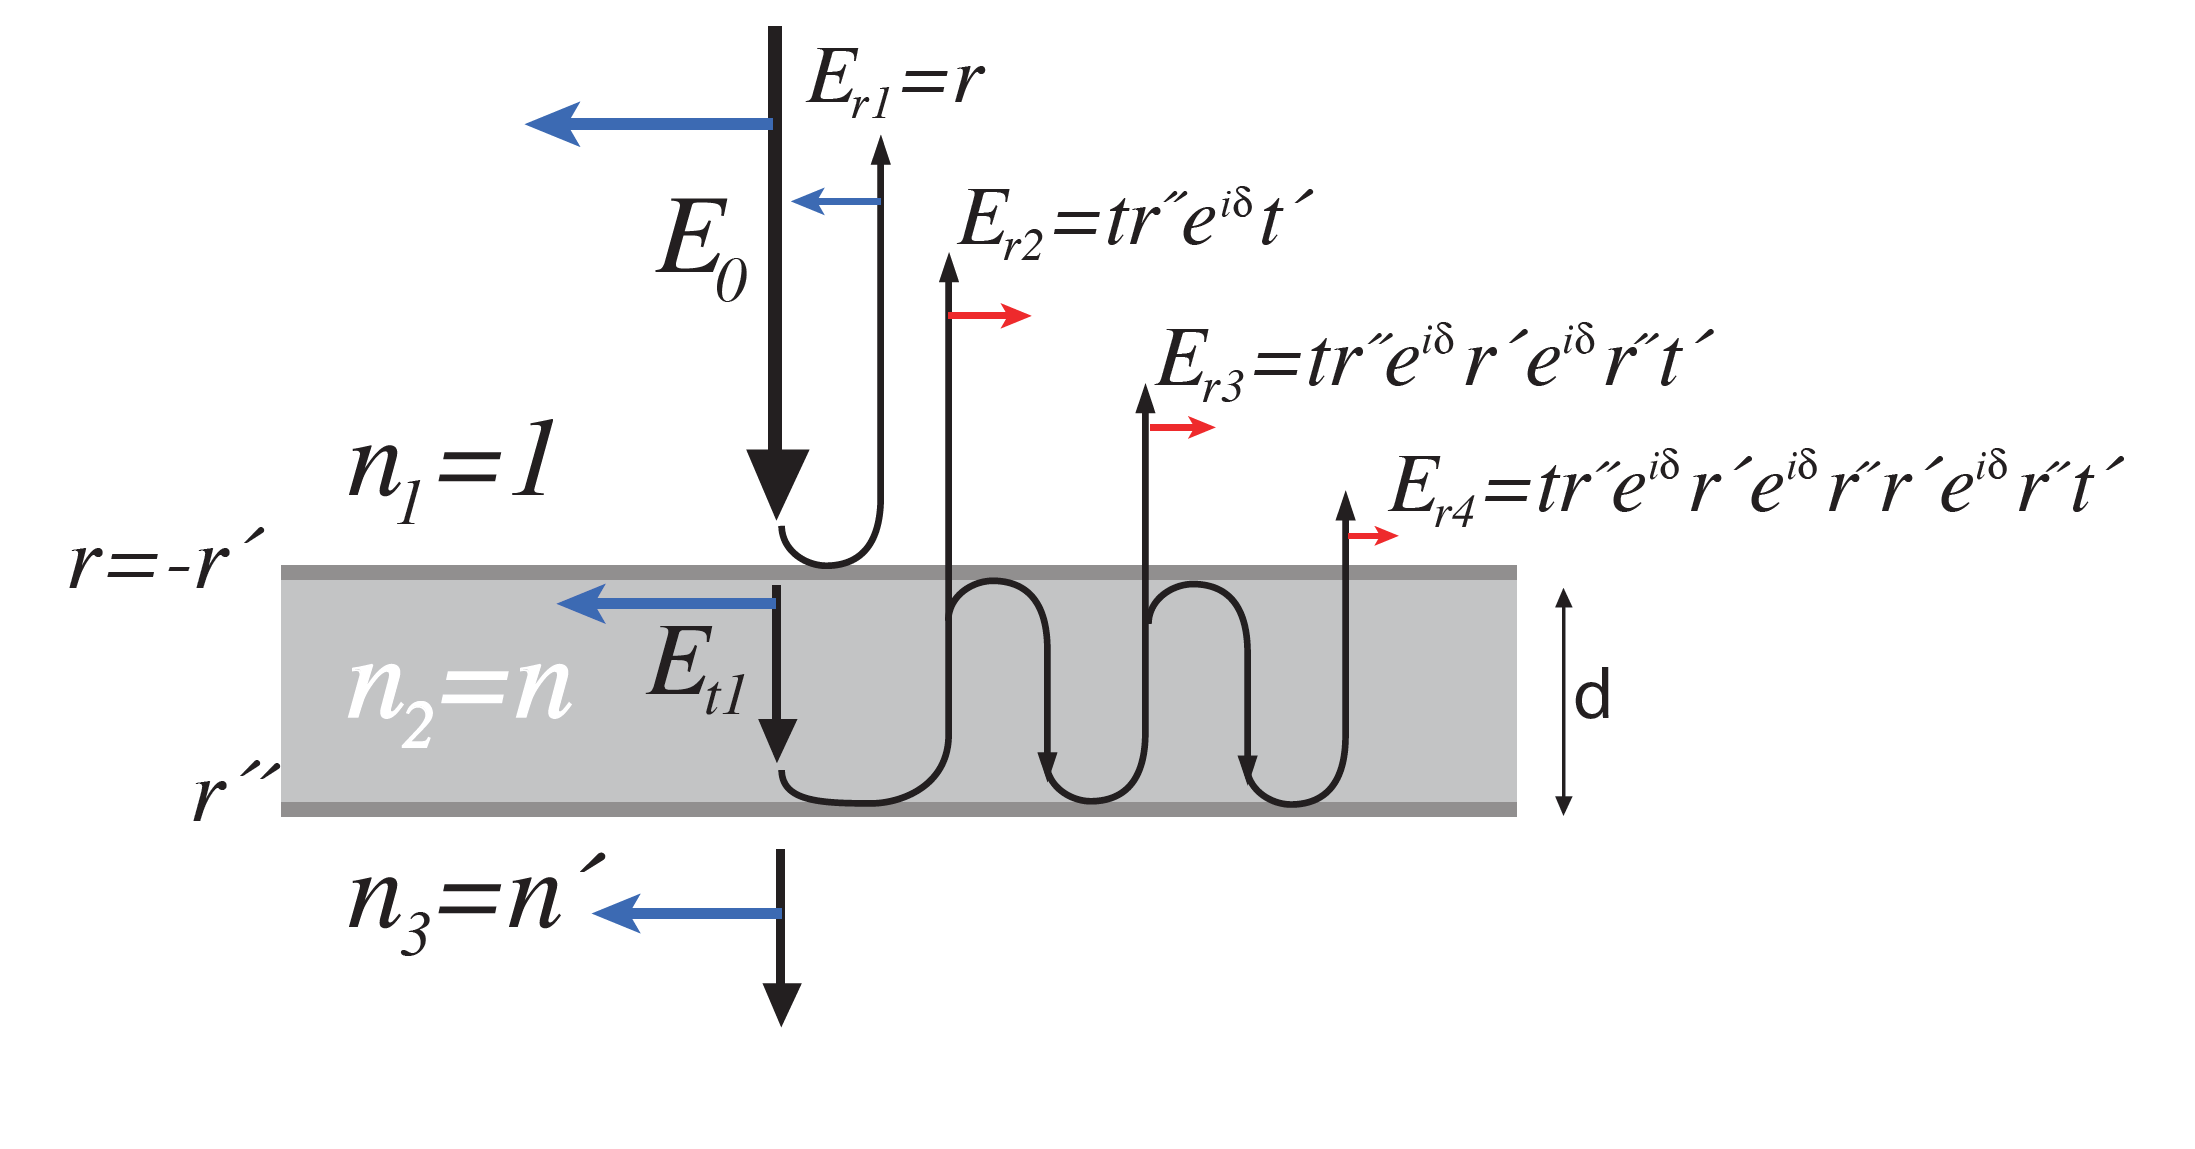
\includegraphics[scale=0.3]{04-DMA.png}
\caption{reflexiones múltiples en una lámina delgada.}
\end{figure}

Es importante recordar la forma de los coeficientes de Fresnel a incidencia normal (como la incidencia normal no importa si estamos en un modo TE y TM, de hecho son indiscernibles a incidencia normal):

\begin{equation}
r=-\frac{n_2-n_1}{n_2+n_1} \tquad t = \frac{2}{n+1}
\label{Ec:04.2-01}
\end{equation}

En este contexto el desfase viene determinado por el incremento de camino óptico $2k_0nd$ por cada ``reflejo''. Si quisieramos calcular el campo total solo tendríamos que sumar: 

\begin{equation}
E_r = \sum_{i=1}^{\infty} E_{ri} = E_i \parentesis{r+e^{i\delta}r''tt'+e^{i2\delta}r''tt'(r'r'')+e^{i3\delta}r''tt'(r'r''r'r'') \cdots}
\end{equation}
Como podemos comprobar esto no es más que una \textit{progresión geométrica} de razón $e^{i\delta}(r''r')$, cuya suma al infinito viene dada por $\sum_n ar^{n} = \frac{a}{1-r}$ (si $r<1$). Con esto último se puede deducir que:

\begin{equation}
E_r = \parentesis{ r + \frac{e^{i\delta}r''tt'}{1-rr''e^{i\delta}}}E_i 
\end{equation}

Esto permite deducir, por ejemplo, cuales son las condiciones de $n$ y $d$ para que la lámina sea completamente antirreflejante $E_r=0$. En primer lugar debe ocurrir que el desfase sea real, esto es, $e^{i\delta}=\pm 1$. Supongamos el caso con signo negativo $e^{i\delta} = -1$, que nos dará el resultado para $n_3>n_2>n_1$. En ese caso $r''$ y $r'$ poseen el mismo signo, por lo que dicha condición es necesaria. Si usamos las \textbf{relaciones de Stokes}, relaciones basadas en la conservación de la energía, obtenemos que

\begin{equation}
\left\lbrace
\begin{array}{ll}
tt'=(1-r^2) & \\
r=-r' &
\end{array}
\right\rbrace
\end{equation}
Estas relaciones se pueden deducir a partir del principio de superposición, inversión temporal y conservación de la energía (óptica I). En cualquier caso, estos coeficientes nos dice que:

\begin{equation}
r = \frac{r'' (1-r^2)}{1+rr''}  
\end{equation}
siendo la solución $r=r''$ lo que nos lleva a deducir, a partir de esto, la relación $n_2(n_3)$ a partir de \ref{Ec:04.2-01} y la el valor de $d$ (recordar que $\delta=\pi$). Entonces las condiciones son:

\begin{equation}
n = \sqrt{n'} \tquad d=(2m+1)\frac{\lambda_0}{4n}
\end{equation}

\subsection{Fórmulas de Airy}

La fórmula de Airy nos da la relación de las intensidades incidente, reflejada y trasmitida cuando iluminamos una lámina delgada de espesor $d$ e índice $n$ en el vacío ($n_1=n_3=1$). Dado que ahora $n_3=1$, tenemos que se verifica que $r''=r'=-r$, por lo que ahora la regresión geométrica viene dada por la razón $r'^2e^{i\delta}$, o lo que es lo mismo

\begin{equation}
E_r = r \ccorchetes{\frac{1-e^{i\delta}}{1-r'^2e^{i\delta}}} E_i
\end{equation}
la irradiancia viene determinada por $I_r=|E_r|^2$. Entonces la \textbf{fórmula de Airy para la intensidad reflejada} viene completamente determinada por

\begin{equation}
I_r =  \ccorchetes{\frac{F \sin^2(\delta/2)}{1+F\sin^2(\delta/2)}} I_i \tquad F = \frac{4r^2}{(1-r^2)^2} = \frac{4R}{(1-R)^2}
\end{equation}
donde a $F$ lo llamamos el \textbf{coeficiente de finura}. Por conservación de energía podemos calcular la \textbf{fórmula de Airy para la intensidad trasmitida}, completamente determinada por

\begin{equation}
I_t = \ccorchetes{ \frac{1}{1+F\sin^2(\delta/2)} }I_i
\end{equation}
Lo interesante ahora sería calcular la fórmula de $\delta$, y estudiar los máximos y mínimos, y la forma del patrón de interferencia para diferentes ángulos de incidencia. Podemos comprobar que el máximo $(\delta=(2m+1)\pi)$ para la intensidad reflejada es el mínimo para la intensidad trasmitida, y el mínimo para la intensidad reflejada $(\delta=2m\pi)$ es el máximo para la intensidad trasmitida. Ahora vamos a calcular la visibilidad para cada uno:

\begin{equation}
\begin{array}{ccc}
I_{r}^{\max} = \ccorchetes{\dfrac{F}{1+F}}I_0 & \tquad I_{r}^{\min} = 0  & \tquad \mathcal{V}_r=1
\\ \\
I_{t}^{\max} = I_0  & \tquad I_{t}^{\min} =  \ccorchetes{\dfrac{1}{1+F}}I_0  & \tquad \mathcal{V}_t=\dfrac{F}{2+F}
\end{array} \label{Ec:04.2-10}
\end{equation}

Ya hemos visto en el tema anterior que para el caso de una lámina plano paralela el desfase $\delta = 2k_0 d_0 n \cos (\theta)$ donde $\theta$ era el ángulo de incidencia sobre la lámina plano-paralela. Si incluimos una lente focal para un $\theta<<1$ (dado que $\sin (\theta) \approx \rho/f$) podemos convertir usar la aproximación del coseno $\cos (\theta) \approx 1 - \frac{\rho^2}{2n^2 f^2}$.

\section{Interferometro de Fabry-Perot}

Un interferómetro Fabry-Perot (FP) está constituido por una lámina plano-paralela de material dieléctrico delimitada por superficies metalizadas de alta reflectancia interna. Si la configuración es simétrica (las láminas plano-paralelas son paralelas entre sí) se peude demostrar que el coeficiente de reflexión $r'$ es exactamente el mismo salvo por un desfase complejo $e^{i \delta_c}$, de tal modo que el nuevo desfase $\delta'=\delta + \delta_c$, aunque $\delta_c>>\delta$. Además ocurrirá que la intensidad $I_0'<I_0$ debido a factores como la \textit{absorción del metal}. Dado que ahora nos interesa el factor 

\begin{figure}[h!] \centering
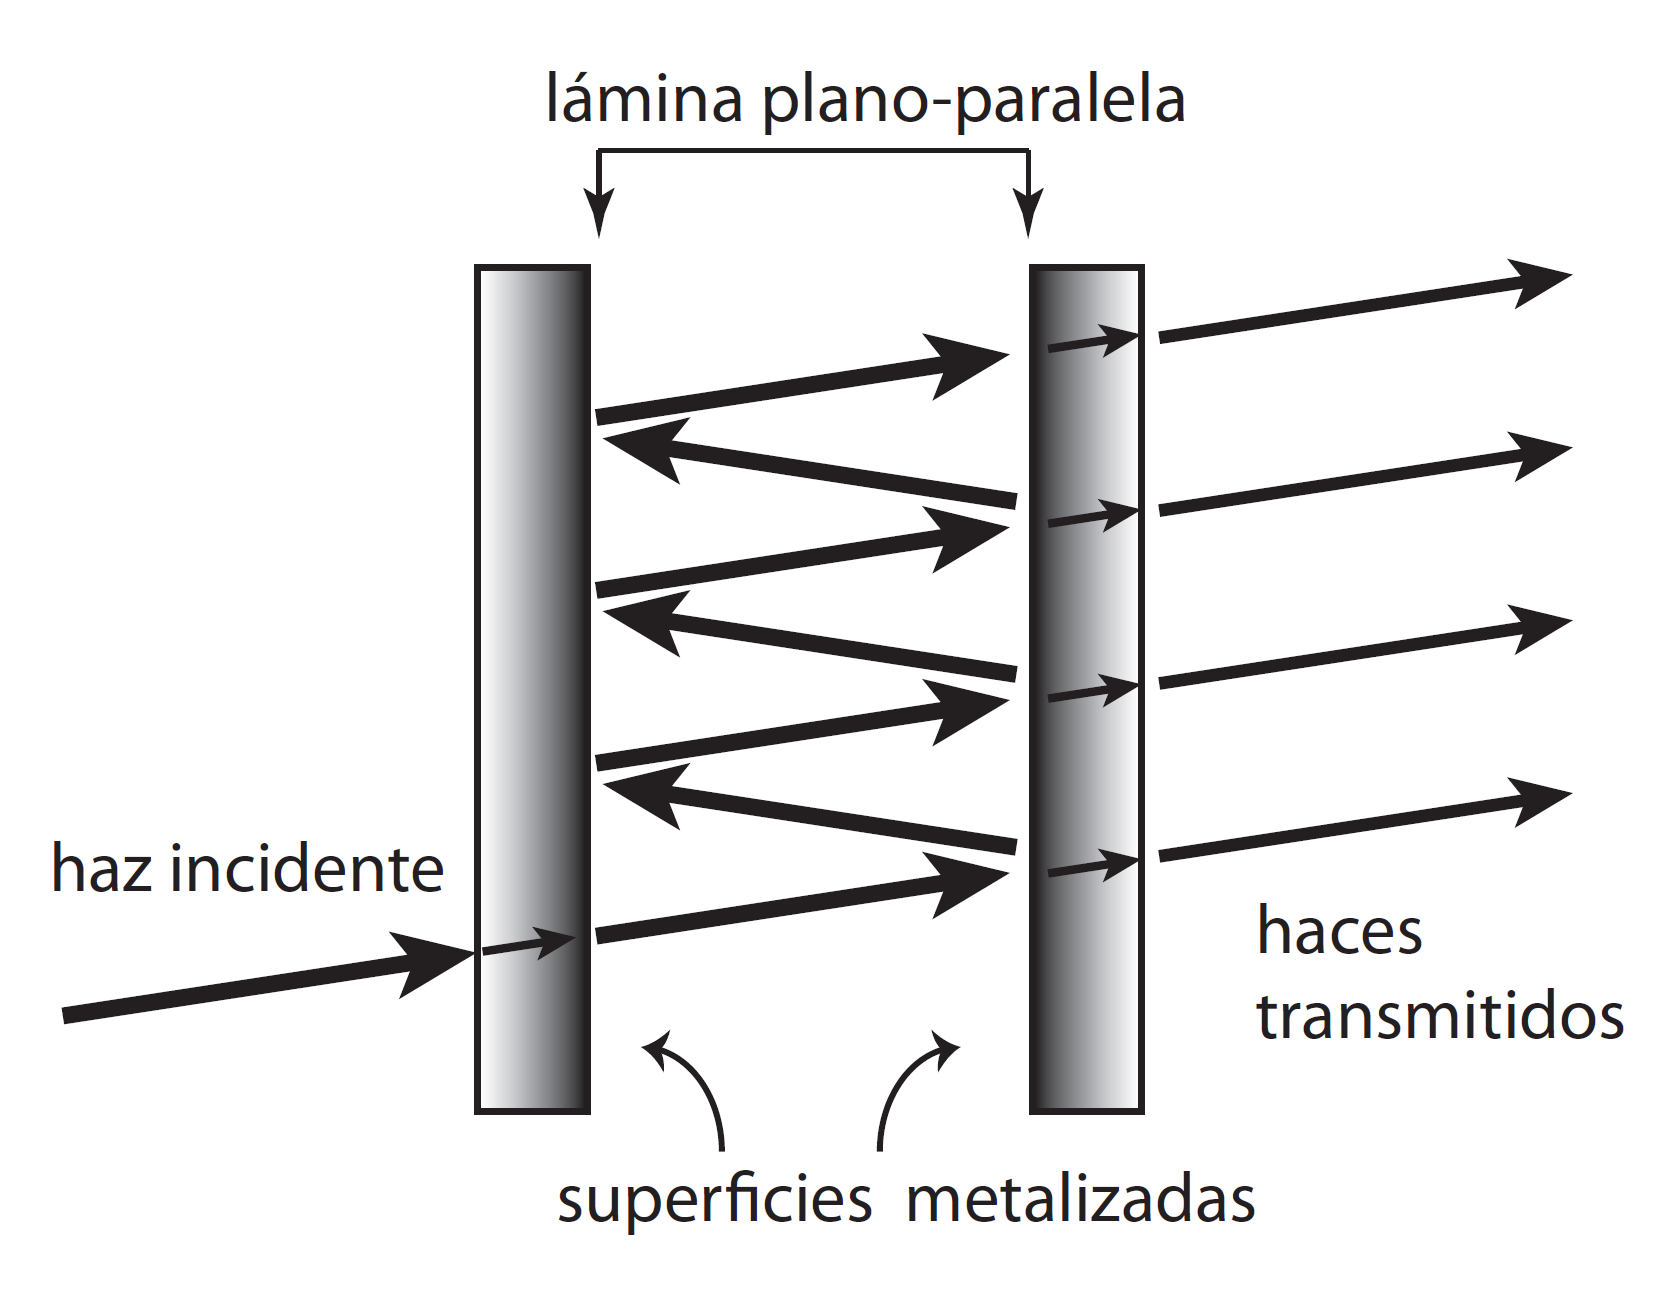
\includegraphics[scale=0.3]{04-Fabry-Perot.png}
\caption{interferómetro Fabry-Perot.}
\end{figure} 

El cálculo debe efectuarse exactamente de la misma manera que en el campo reflectido total anterior. Entonces tenemos que:

\begin{equation}
E_t = \ccorchetes{tt't_mt_m'\parentesis{1+r'r'_m e^{i\delta'} + (r'r_m')^2e^{2\delta'}+(r'r'_m)^3e^{i3\delta'} + \cdots}} E_i
\end{equation}
De este modo tenemos que la razón de la progresión geométrica es:

\begin{equation}
E_t = \ccorchetes{\frac{tt_mt't_m'}{1-(r'r_m')e^{i\delta'}}} E_i
\end{equation}
Desarrollando la ecuación de la intensidad trasmitida $I_t = |E_t|^2$:

\begin{equation}
I_t = \ccorchetes{ \frac{1}{1+F'\sin^2(\delta'/2)}}I_0' \tquad I_0' = \ccorchetes{\frac{tt_m t't_m'}{1-R'^2}} I_0 \tquad F=\frac{4R'}{(1-R')^2}
\end{equation}
finalmente la ecuación de la trasmitida:

\begin{equation}
I_r =\ccorchetes{\frac{F' \sin^2(\delta'/2)}{1+F' \sin^2(\delta'/2)}} I_0'
\end{equation}
Se puede comprobar que la visibilidad es exactamente la misma que  la vista en la ecuación \ref{Ec:04.2-10}. La única diferencia es que $\delta \rightarrow \delta'$. Tendremos el mínimo de la intensidad trasmitida en $\delta'=2m\pi$, y el máximo de la intensidad trasmitida en $\delta'=(2m+1)\pi$. Tendremos el mínimo de la intensidad reflejada en $\delta'=(2m+1)\pi$ y el mínimo de la intensidad reflejada en $\delta'=2m\pi$. 

\begin{equation}
\begin{array}{ccc}
I_{r}^{\max} = \ccorchetes{ \dfrac{F}{1+F}}I_0' & \tquad I_{r}^{\min} = 0  & \tquad \mathcal{V}_r=1
\\ \\
I_{t}^{\max} = I_0'  & \tquad I_{t}^{\min} = \ccorchetes{\dfrac{1}{1+F} }I_0' & \tquad \mathcal{V}_t=\dfrac{F}{2+F}
\end{array}
\end{equation}

Como podemos ver para finuras muy grandes tendremos unas franjas muy estrechas. Si por ejemplo recogiéramos los patrones interferenciales  usando el plano focal de una lente, dada la simetría de la lente obtendríamos franjas esféricas muy finas, tal y como podemos ver en la figura \ref{Fig:04.3-04}. En la figura podemos ver la representación en el espacio fásico \ref{Fig:04.3-03}. 


\begin{figure}[h!] \centering
\begin{subfigure}[m]{0.45\linewidth} \centering
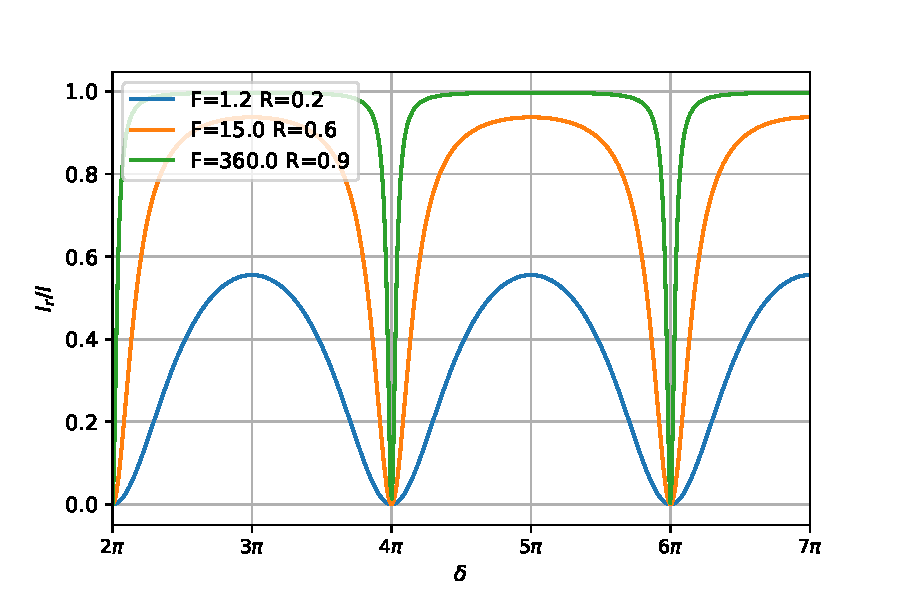
\includegraphics[scale=0.5]{04-Ir.pdf}
\end{subfigure}
\begin{subfigure}[m]{0.45\linewidth} \centering
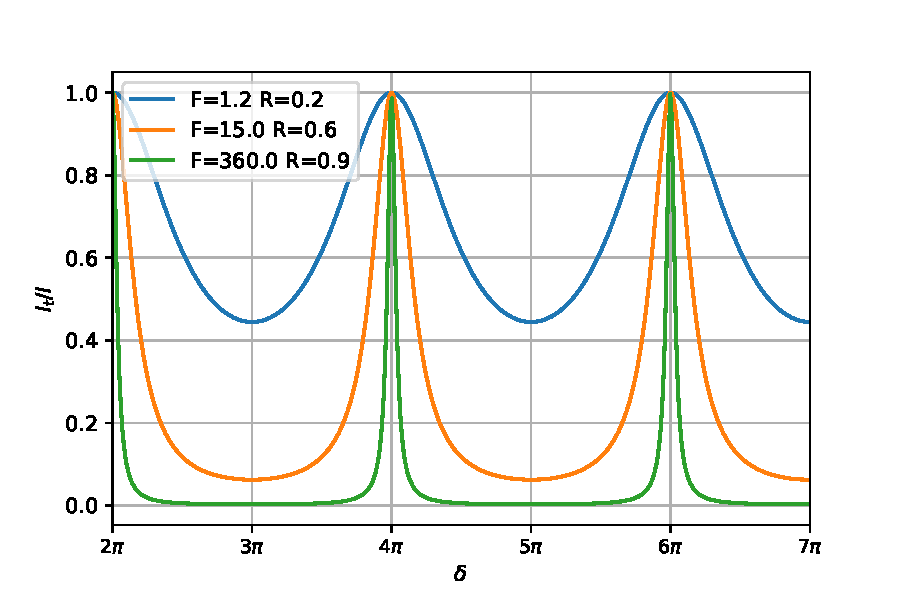
\includegraphics[scale=0.5]{04-It.pdf}
\end{subfigure}
\caption{valores de $I_r$ e $I_t$ para diferentes valores de $\delta'$.}
\label{Fig:04.3-03}
\end{figure}

\begin{figure}[h!] \centering
\begin{subfigure}[m]{0.45\linewidth} \centering
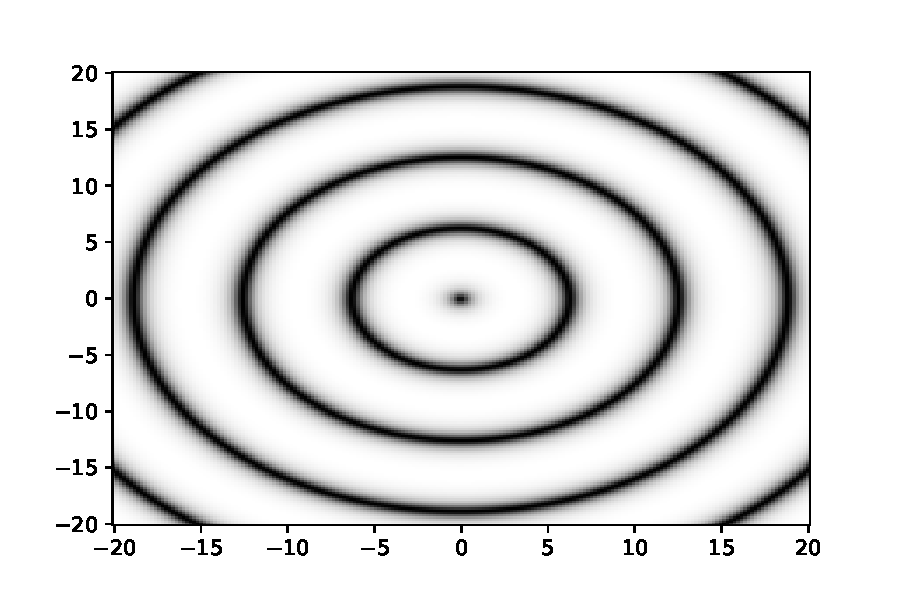
\includegraphics[scale=0.5]{04-Fabry_Perot_It-F15.pdf}
\caption{bandas $I_t$ para finura $F=$15.}
\end{subfigure}
\begin{subfigure}[m]{0.45\linewidth} \centering
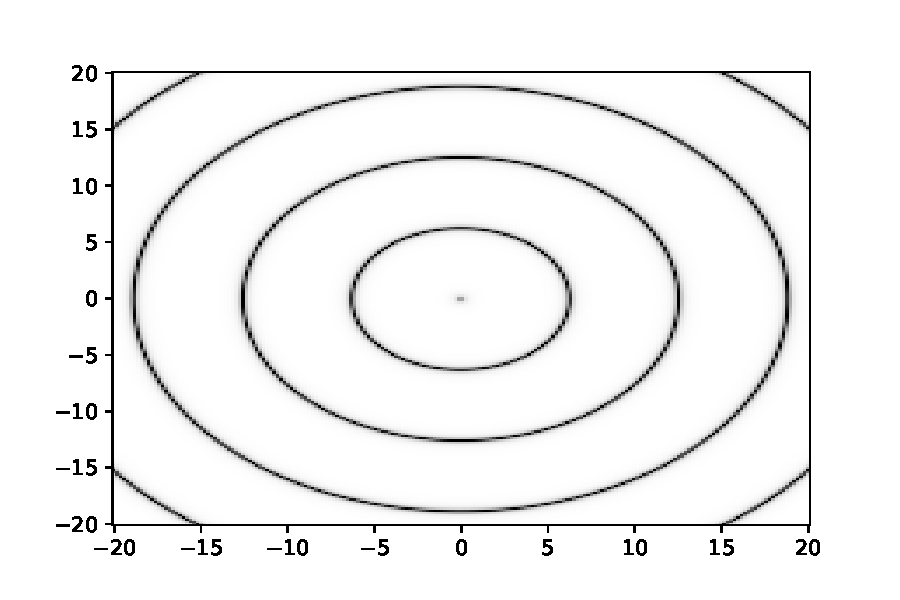
\includegraphics[scale=0.5]{04-Fabry_Perot_It-F360.pdf}
\caption{bandas $I_t$ para finura $F=$360.}
\end{subfigure}
\caption{bandas esféricas para $I_t$ en el plano $XY$.}
\label{Fig:04.3-04}
\end{figure}



\subsection{Análisis espectral de la intensidad interferncial}

En las aplicaciones espectroscópicas no solo es de interés el coeficiente de finura, también es importante su coeficiente de \textbf{fineza} $\mathcal{F}$. El coeficiente de fineza es una medida de la anchura de cada uno de los picos. Una buena medida de la fineza podría ser la diferencia espectral entre los máximos ($2\pi$, tal y como se puede ver en la imagen \ref{Fig:04.3-03}) entre el inverso de la anchura total de cada uno de los picos. Definamos la \textbf{anchura fásica total} $\gamma$ como la distancia $\Delta \delta'=\delta_+'-\delta_-'$, donde $\delta_+'$ y $\delta_-'$ son los $\delta'$ que verifican que la intensidad se reduce a la mitad. Esto es:

$$ \frac{1}{2} = \frac{1}{1+F\sin^2(\delta_{\pm}'/2)} \rightarrow \sin (\delta'_\pm/2) = \pm \frac{1}{\sqrt{F}} $$
entonces si suponemos la aproximación a ángulos pequeños tal que $\sin (\delta'/2) \approx \delta'/2$, lleva a la expresión $\delta_{\pm}=\pm2/\sqrt{F}$.

\begin{equation}
\gamma = \frac{4}{\sqrt{F}}
\end{equation}
Entonces definimos la \textbf{fineza} $\mathcal{F}$ como el cociente entre la distancia entre máximos y la anchura del pico, esto es:

\begin{equation}
\mathcal{F} = \frac{\pi \sqrt{F}}{2}
\end{equation}

\subsection{Poder de resolución}

Un sistema se puede resolver cuando los patrones producidos por la superposición de varios sistemas de franjas (doblete atómico, fuente policromática) son individualmente distinguibles. El parámetro que permite medir esta capacidad es el \textit{poder de resolución}, que se define como el cociente entre el parámetro qeu define a la magnitud evaluada y la mínima diferencia de valores de esta magnitud que resultan distinguibles, como pueden ser

\begin{equation}
PR = \frac{\omega}{\Delta \omega} = \frac{\nu}{\Delta \nu} = \frac{\lambda}{\Delta \lambda}
\end{equation}

Entre los muchos criterios que existe uno de los más interesantes es el \textbf{criterio de Taylor}. El criterio de Taylor dice que dos líneas espectrales de igual orden e igual intensidad se consideran resueltos si ambas intersectan a la \textit{mitad de la intensidad máxima}. Otro criterio interesante es el \textbf{criterio de Rayleigh} que establece otro valor límite para la $I_T$ que se pueden sumar las dos líneas en el punto intermedio $I_T=(8/\pi^2)I_0$. \\

\shadowbox{\textbf{Doblete atómico}}

\hrulefill

Consideremos una fuente que emite a dos frecuencias muy próximas con la misma intensidad $I_0$. En la focal de la lente tendremos la superposición de patrones de interferencia. Dado que la emisión de las ondas de diferentes frecuencias es independiente, la intensidad observada será la suma de las intensidades interferenciales emitidas por la fuente. 

\begin{equation}
I_T = I_0 \ccorchetes{\frac{1}{1+F\sin^2(\delta/2)}} + I_0 \ccorchetes{\frac{1}{1+F\sin^2(\delta/2)}}
\end{equation}
Según el criterio de Taylor en el punto medio entre los máximos la intensidad debe ser de $I_0$. La distancia mitad entre los dos máximos viene dada por $\Delta/2=(\delta'-\delta)/2$. Como en dicho punto cada una de las intensidades debe valer $I_0/2$ debe verificarse que:

$$ I_0 \ccorchetes{\frac{1}{1+F\sin^2(\delta/2+\Delta/4)}} = \frac{I_0}{2} \tquad I_0 \ccorchetes{\frac{1}{1+F\sin^2 \parentesis{\delta'/2-\Delta/4}}} = \frac{I_0}{2} $$
Dado que están evaluados en el máximo debe verificarse que $\delta=\delta'=2m\pi$, y como $\sin^2m\pi+\theta) = \sin^2(\theta)$, y $\sin^2(-\Delta/4) = \sin^2(\Delta/4)$, tenemos que ambas exigen la misma condición dada por (falta desarrollo algebraico sencillo para el lector):

\begin{equation}
\sin^2(\Delta /4) = \frac{1}{F} \label{Ec:04.3-20}
\end{equation}
Sea $\Delta<<1$, entonces de la ecuación \ref{Ec:04.3-20} podemos deducir ($\sin (\Delta) \approx \Delta/4$):

\begin{equation}
|\delta'-\delta|=\frac{4}{\sqrt{F}}
\end{equation}
Si $\delta=2nk_0d\cos \theta$ siendo $\theta$ el ángulo de incidencia y $k_0=\omega/c$. Si además $\theta \approx \theta'$, lo que podemos asumir como cierto, ya que prácticamente proceden de la misma ``fuente puntual'', entonces $|\delta'-\delta|= (2n\cos(\theta)/c)\Delta\omega$, de lo que deducimos la expresión:


\begin{equation}
\Delta \omega = \frac{c}{2nd\cos (\theta)} \frac{4}{\sqrt{F}}
\end{equation}
De este modo el \textbf{poder de resolución}

\begin{equation}
PR = \frac{\omega_{\max}}{\Delta \omega} = \frac{\frac{c}{2nd\cos(\theta)} \delta_{\max}}{\frac{c}{2nd \cos (\theta)} \frac{4}{\sqrt{F}}} = \delta_{\max} \frac{\sqrt{F}}{4} = 2m\pi \frac{\sqrt{F}}{4} )= m \mathcal{F}
\end{equation}
\hrulefill


\section{Láser (aplicación Fabry-Perot)}

El \textbf{láser} (Light Amplification by Stimulated Emission of Radiation) consiste esencialmente en una cavidad resonante Fabry-Perot de separación $d$ con caras de altísima reflectancia $R=1$ y $R\approx1$ que encierra a un emisor que tras ser sometido a excitación con energía genera una luz altamente coherente. 

\subsection{Resonador óptico}

Consideremos la cavidad resonante y las ondas electromagnéticas en su interior. Supongamos que el \textit{medio activo} (medio donde tiene lugar la excitación) tiene un índice de refracción $n$. Sin pérdida de generalidad podemos asumir que la normal de los espejos son paralelos al eje $z$. La superposición de ondas electromagnéticas en esa cavidad limitada por dos superficies planas generará ondas estacionarias que deben verificar, en las superficies de los espejos, el campo es cero ($E|_{z=0}=E|_{z=d}=0$). Esta condición debe verificarse ya que el campo trasmitido es prácticamente nulo. En ese caso la onda estacionaria 

\begin{equation}
E(\rn) = E(x,y) \sin (k_m z)
\end{equation}
De lo que se puede deducir la condición $\sin(k_md)=0\longrightarrow k_m=m\pi/d$. A su vez, de esto podemos deducir las frecuencias permitidas en la cavidad debido a la no infinitud de nuestro láser. En ese caso las frecuencias permitidas son:

\begin{equation}
\nu_m = \frac{\omega_m}{2 \pi} = \frac{k_m}{2 \pi} \frac{c}{n} = \frac{1}{\lambda_m} \frac{c}{n} = \frac{m}{d}\frac{c}{2n}
\end{equation}
A las frecuencias permitidas se les llama \textbf{modos longitudinales} o \textbf{modos temporales}. Estas frecuencias son efectivamente aquellas en las que se produce máximos de intensidad de trasmisión, tales que

\begin{equation}
\frac{I_t}{I_i} = \frac{1}{1+F \sin^2 (\delta/2)}
\end{equation}
donde $\delta=k_mnd\cos (\theta')$, siendo $\theta$ el ángulo de incidencia y $\theta'$ el de trasmisión. Aunque tampoco se debe ser ingenuo, existen muchos otros factores que limitan la cantidad de frecuencias que puede existir en una de estas cavidades (energéticos, cuánticos...). \\

Uno de los factores mas importantes es que, además de tener dichas superficies, tiene otras 4 paredes que encierran la cavidad. Esto en realidad crea una cantidad ingente de modos de resonancia, dadas por la ecuación de Helmholtz y las condiciones de contorno, que cambian en función de las distancias entre las paredes de las cajas, o en el caso de ser un cilindro del radio... \\

Por razones de estabilidad los láseres se construyen con \textit{espejos esféricos} cuya curvatura se ajuste a la de los frentes de ondas gaussianos y por tanto reflejan éstos múltiples veces. Esto se consigue ajustando la suma de los focos de ambos espejos a un valor igual o menor a la separación entre ellos (configuración confocal). 

\subsection{Amplificación cuántica de la luz}

Definimos como \textbf{emisión estimulada} a aquella que es devida a la presencia de radiación en el entorno de los átomos que bajo interacción los des-excita. La des-excitación produce pares de fotones que tienen la misma fase, frecuencia, polarización y dirección que las de los excitadores. \\

\begin{figure}[h!] \centering
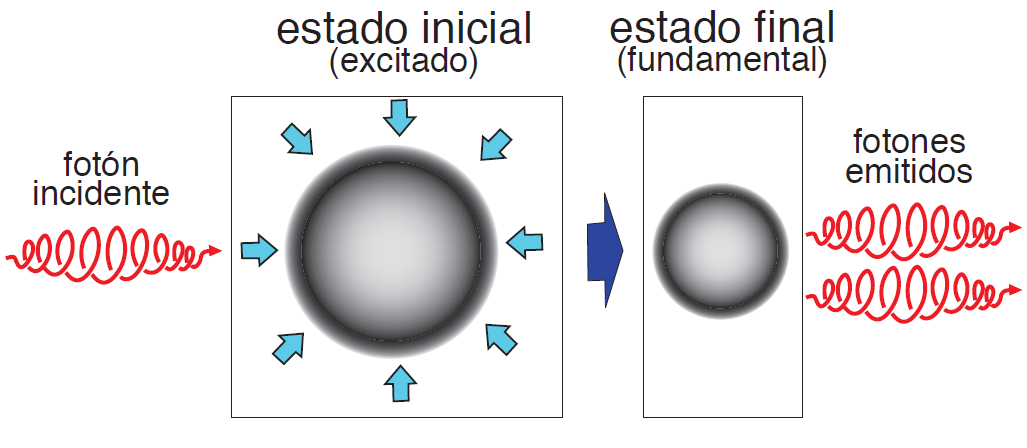
\includegraphics[scale=0.6]{04-Emision_estimulada.png}
\caption{fenómeno de la emisión estimulada.}
\label{Fig:04.5-05}
\end{figure}

\section{Óptica de multicapas}

Lo que haremos en esta sección es estudiar el comportamiento de una onda electromagnética procedente de un medio $n_0$ en un medio de índice de refracción $n_1$. Este último medio se encuentra a su vez sobre otro medio, el llamado \textbf{sustrato}, con un medio de índice $n_s$. La acción de las capas sobre la onda es un proceso de interferencia múltiple. A diferencia de la primera parte del tema, donde hemos supuesto una incidencia normal, en este supondremos que el ángulo de incidencia sobre la primera lámina es $\theta_0$. Debido a esto último el modo de la onda (\textit{modo transversal eléctrico} o \textit{modo transversal magnética}) tendrá relevancia. \\

El \textit{quid} de la cuestión es hallar la forma de $r$ e función y $t$ en función de los ángulos de incidencia y los índices de refracción $n_1,n_s$. Dado que el título de la sección se llama \textit{óptica de multicapas} lógicamente trataremos de generalizar el resultado para $N$ capas dieléctricas. \textit{Grosso modo} lo que haremos será buscar las relaciones $E_1(E_i,H_i)$  y $H_1(E_i,H_i)$ usando las \textit{condiciones de continuidad}. Así hallaremos una relación matricial, de donde luego podremos despejar $E_i$, gracias a la ecuación

\begin{equation}
\Hn_i = \sqrt{\varepsilon_0/\mu_0} n (\kn_0 \wedge \En) \label{Ec:04.5-26}
\end{equation}
De aquí podremos obtener las relaciones $E_1\propto E_i$ y $H_1 \propto E_i$. Dicha ecuación matricial nos servirá para hallar los parámetros $r$ y $t$ en función de las condiciones del problema ($n_1,n_2,...,n_N,d_1,d_2,...,d_N,\theta_i$). Se que puede parecer complicado, pero quedará mas claro en cuanto lo hagamos. Las condiciones de continuidad se deducen a partir de las \textbf{ecuaciones de Maxwell} (ver \cite{libro-1} para mas detalles)

\begin{equation}
\left\lbrace
\begin{array}{lll}
E_{1t} & = & E_{t2}  \\ 
D_{1n} & = & D_{2n} \\
H_{1t} & = & H_{2t} \\
B_{1n} & = & B_{2n} \\
\end{array}
\right.
\end{equation}

\begin{figure}[h!] \centering
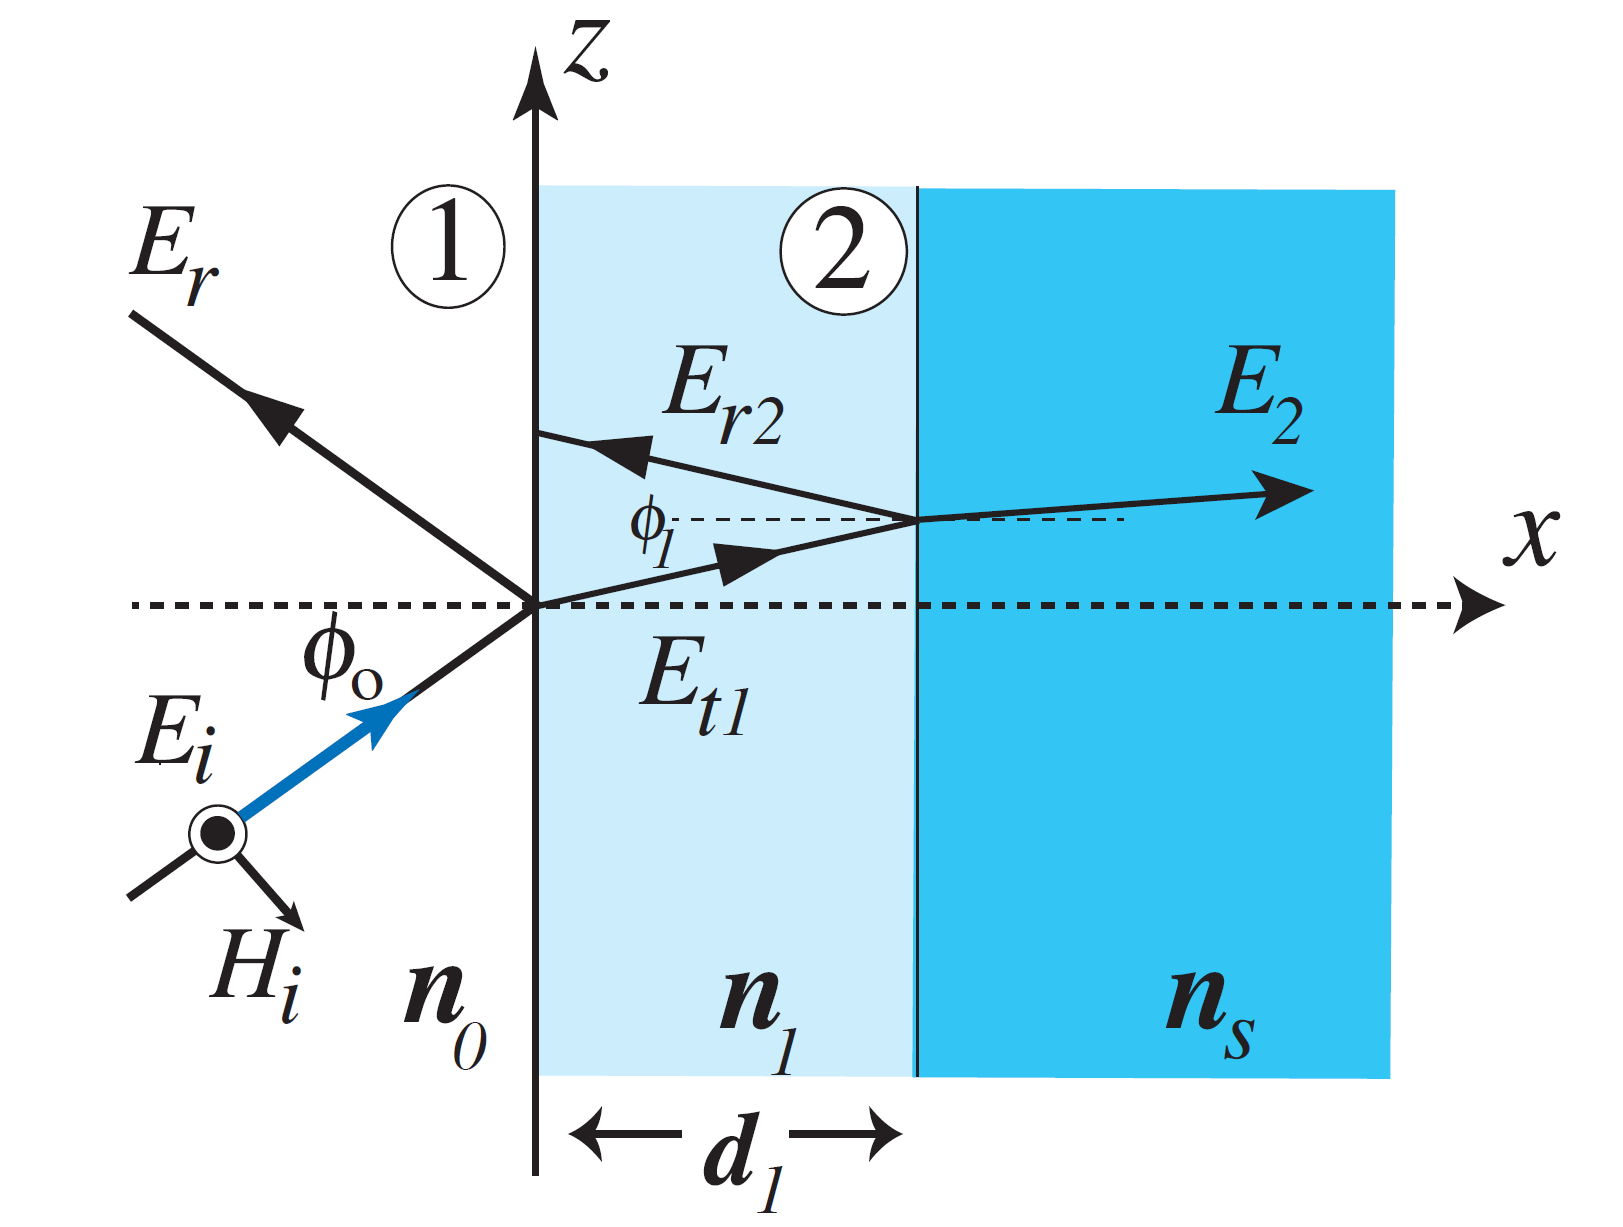
\includegraphics[scale=0.35]{04-Multicapas.png}
\caption{Esquema práctico para resolver las multicapas.}
\label{Fig:04.5-06}
\end{figure}

Primero tendremos que seleccionar un modo de oscilación. Sea pr ejemplo un modo TE tal y como se puede ver en la imagen \ref{Fig:04.5-06}. Sea $E_0=E_i-E_r$ y $E_1=E_{t1}-E_{r2}$. Diferenciaremos las condiciones de la primera interfase y de la segunda interfase:

\begin{itemize}
\item Aquí evaluaremos las condiciones de continuidad de la primera interfase. La condición del campo eléctrico es:

\begin{equation}
E_1=E_i+E_r=E_{t1}+E_{r2}
\end{equation}
y la condición del campo magnético:

\begin{equation}
H_1 = H_i + H_r = H_{t1} + H_{r2} \tquad  H_1= \gamma_0 (E_i-E_r)   = \gamma_1 (E_{t1} - E_{r2})
\end{equation}
donde hemos usado los siguientes coeficientes

\begin{equation}
\gamma_0 = \sqrt{\frac{\varepsilon_0}{\mu_0}} n_0 \cos(\phi_0) \tquad 
\gamma_1 = \sqrt{\frac{\varepsilon_0}{\mu_0}} n_1 \cos(\phi_1)
\end{equation}
siendo el coseno un resultado de las condiciones de continuidad, y el signo negativo delante de $E_r$ ya que $k_{0x}\rightarrow -k_{0x}$ al ser una onda regresiva.

\item Aquí evaluaremos las condiciones de continuidad de la segunda interfase. La segunda interfase verifica las mismas ecuaciones de antes salvo por el factor de recorrido óptico. En ese caso tenemos que por continuidad del campo eléctrico:

\begin{equation}
E_{t1}e^{i \delta} -E_{r2}e^{-i \delta} = E_2
\end{equation}
el factor $-\delta$ proviene de que el valor evaluado del campo $E_{r2}$ esta en la interfase 1, por lo que aun tiene que recorrer dicho camino añadiendo esa fase. Para que se cancele debe tener el signo $-$. Por continuidad del campo magnético:

\begin{equation}
H_2=\sqrt{\frac{\varepsilon_0}{\mu_0}} n_1 \parentesis{
\cos (\phi_1) E_{t1}e^{i \delta} - \cos (\phi_2) E_{r2}e^{i \delta}} = \gamma_1 \parentesis{E_{t1}e^{i \delta} -E_{r2}e^{i \delta}}
\end{equation}
donde $\delta = n_1k_0d_1 \cos (\phi)$ ya que el camino óptico relevante es el que tiene lugar en la dirección $x$, y $\kn=k_0(\cos(\theta_1)x+\sin(\theta_1)z)$
\end{itemize} 
Como podemos ver la relación entre $H_2,E_2$ y $H_1,E_1$ es la siguiente:

\begin{equation}
\begin{pmatrix}
E_1 \\
H_1
\end{pmatrix}
= 
\begin{pmatrix}
\cos (\delta_1) & -(i/\gamma_1)\sin (\delta_1) \\
-(i\gamma_1)\sin(\delta_1) & \cos (\delta_1 )
\end{pmatrix}
\begin{pmatrix}
E_2 \\
H_2
\end{pmatrix}
=
\mathcal{M}_1 
\begin{pmatrix}
E_2 \\
H_2
\end{pmatrix}
\end{equation}
tras $N$ capas dieléctricas con $N$ índices $n_1,n_2,...$ y $N$ grosores $d_1,d_2...$, tenemos la matriz:

\begin{equation}
\mathcal{M} = \mathcal{M}_1\mathcal{M}_2 \cdots \mathcal{M}_N = \begin{pmatrix}
m_{11} & m_{12} \\
m_{21} & m_{22}
\end{pmatrix}
\end{equation}
donde $\mathcal{M}$ es la llamada \textbf{matriz característica} de la multicapa. Teniendo en cuenta que $E_{N+1}\equiv E_t = tE_i$ y que $H_{N+1}\equiv \gamma_s E_t = \gamma_s t E_i$. Si ademas tenemos que $E_r=rE_i$, tal que $E_1=(1+r)E_i$. Despejando esto último tenemos la ecuación:


\begin{equation}
\begin{pmatrix}
(1+r) \\
\gamma_0 (1-r)
\end{pmatrix} = \mathcal{M}
\begin{pmatrix}
t \\
\gamma_s 
\end{pmatrix}
\end{equation}
despejando la ecuación podemos llegar a la expresión final de $r$ y $t$ en función de los parámetros que queríamos, esto es:

\begin{equation}
r=\frac{\gamma_0 m_{11} + \gamma_0 \gamma_s m_{12} - m_{21} - \gamma_s m_22}{D} \tquad t = \frac{2\gamma_0}{D}
\end{equation}
donde $D=\gamma_0 m_{11} + \gamma_0 \gamma_s m_{12} + m_{21} + \gamma_s m_{22}$. \\


\shadowbox{\textbf{Caso doble capa}}

\hrulefill


El caso de dos capas es un caso importante en la industria óptica. Sea un rayo incidiendo normalmente ($\phi_i=0$). En ese caso $\delta_1 = k_0 n_1 d_1$ para la primera capa y $\delta_2=k_0n_2d_2$ para la segunda. Si se verifica la condición $\delta_1=\delta_2=(2m+1/2)\pi$ (para simplificar, se puede elegir otra):

\begin{equation}
(2m+1/2)\pi = \frac{2\pi}{\lambda_0} n d \Longrightarrow nd= \frac{\lambda}{4} \parentesis{4m+1} 
\end{equation}
de este modo tenemos que:

\begin{equation}
\mathcal{M}_1 =  \begin{pmatrix}
0 & -i/n_1 \\
-i n_1 & 0
\end{pmatrix} \tquad 
\mathcal{M}_2 = \begin{pmatrix}
0 & -i/n_2 \\ 
- i n_2 & 0
\end{pmatrix}
\end{equation}
y por tanto:

\begin{equation}
\mathcal{M} = \begin{pmatrix}
-n_2/n_1 & 0 \\
0 & -n_1/n_2
\end{pmatrix}
\end{equation}
de lo que se deduce la relación $r$, tal que:

$$r = \frac{n_0 n_2/n_1-n_sn_1/n_2}{n_0 n_2/n_1 +n_s n_1/n_2 }$$
dejándolo limpio:

\begin{equation}
r=\frac{n_0n_2^2-n_sn_1^2}{n_0n_2^2+n_sn_1^2}
\end{equation}
Para que se verifique la condición de \textbf{antirreflejancia} $R=r=0$ debe cumplirse entonces:

\begin{equation}
\frac{n_2}{n_1} = \sqrt{\frac{n_s}{n_0}}
\end{equation}


\hrulefill


\subsection{Sistemas periódicos de multicapas}

Una forma de mejorar la reflectancia y la trasmictancia es hacer sistemas periódicos de bicapas $H$ y $L$ de espesor $\lambda/4$. Llamaremos $H$ a la capa de mayor índice y $L$ a la capa de menor índice (de Hight y Low). La bicapa LH tenemos que

\begin{equation}
\mathcal{M} = \mathcal{M}_L \mathcal{M}_H = 
\begin{pmatrix}
-\frac{n_H}{n_L} & 0\\
0 & -\frac{n_L}{n_H}
\end{pmatrix}
\end{equation}
Ahora, si colocáramos $N$ bicapas juntas tal que $\mathcal{M}_N=\mathcal{M}^N$, tendríamos una reflectancia de:

\begin{equation}
R = \left| \frac{(n_H/n_L)^{2N}-1}{(n_H/n_L)^N+1} \right|^2
\end{equation}
La nomenclatura de estos sistemas periódicos es la siguiente: $s(HL)^Na$.
 
\subsection{Filtros interferenciales o filtros Fabry-Perot}

Si hicieramos un montaje con una disposición del tipo $aLH...HLLH...HLs$ debido a la propiedad de las láminas de espesor $\lambda_4$, que verifican:

\begin{equation}
\mathcal{M}_L^2 = \mathcal{M}_H^2 =  -\mathbb{I}
\end{equation}
obtendríamos que, tras $N$ multiplicaciones, la  matriz final vendría dada por:

\begin{equation}
\mathcal{M} = \mathcal{M}_L \mathcal{M}_H \cdots \mathcal{M}_H \mathcal{M}_L
\mathcal{M}_L \mathcal{M}_H \cdots \mathcal{M}_H \mathcal{M}_H = \mathbb{I}
\end{equation}
De este modo estamos seleccionando una longitud de onda $\lambda_0$ que verifica $n_Hd_H = n_L d_L = \lambda_0 /4$. Esto es, estamos construyendo una cavidad Fabry-Perot

\newpage

\chapter{Teoría de difracción óptica} \label{Sec:5}

En este capítulo vamos a tratar de familiarizarnos con el concepto de difracción óptica,  entendiéndola como la interacción microscópica de luz-materia que perturba la fase y/o amplitud. Comprenderemos las hipótesis de diferentes toerías (Kirchoff, Sommerfeld...) y su formalización en las correspondientes integrales de difracción (integrales de difracción de Huygends-Fresnel-Young) aproximadas para comprender el concepto de difracción aproximada para comprender el concepto de difracción y conocer las vías alternativas de formalización del campo difractado. Además estudiaremos las condiciones de paraxialidad para la determinación del campo óptico difractado por obstáculos tanto de amplitud como de fase, la interpretación de las integrales de difracción de Fresnel y Fraunhofer, conocer y saber aplicar el principio de Complementariedad o de Babinet, entender y saber formalizar la teoría difraccional de la imagen. 

\section{Formalismo de la difracción.}

Un cuerpo opaco colocado a medio camino entre una pantalla y una fuente puntual proyecta una sombra complicada hecha de regiones claras y oscuras muy diferentes de las que podría esperarase de los principios de la óptica geométrica. El trabajo de Francesco Grmimaldi en el siglo XVII fue el primer estudio detallado qeu se publicó sobre esta \textbf{desviación de la luz de su propagación rectilínea}, a la que denominó ``difracctio''. \textit{El efecto es una característica general de los fenómenos ondulatorios que ocurren siempre que una parte de un frente de onda, ya sea sonido, onda material o luz, esté obstruida de alguna manera}. Si al encontrar un obstáculo, sea trasparente (como una lente) o opaco (una pared) se altera la amplitud o la fase de una región del frente de odna, se producirá difracción. No existe una distinción física significativa entre interferencia y difracción, sin embargo se ha hecho común hablar de interferencia cuando se analiza la superposición de unas pocas odnas y de difracción cuando se trata de un gran número de estas ondas. Las alteraciones de amplitud y fase propias de los obstáculos se formalizan mediante una \textbf{función de trasmisión} $t(x_0,y_0)$. Las alteraciones más comunes son las siguientes: \\

\begin{itemize}
    \item \textbf{Abertura}: alteración binaria de amplitud (la región $\mathsf{A}$ deja pasar la luz y $\bar{A}$ la región complementaria no deja pasar la luz) sin alteración de la fase. La función de trasmisión:

    \begin{equation}
        t_A(x_0,y_0) = \left\lbrace \begin{array}{cc}
            1 & (x_0,y_0) \in \mathsf{A} \\
            0 & (x_0,y_0) \in \mathsf{\bar{A}}
        \end{array} \right.
    \end{equation}
    
    \item \textbf{Lente}: la acción de una lente, considerada puramente de fase y su amplitud constante $|t_L (x_0,y_0)|=1$. 
    
    \begin{equation}
        t_L(x_0,y_0) = e^{-ik_0\parentesis{\frac{x_0^2+y_0^2}{2f}}}
    \end{equation}
\end{itemize}
El efecto difractivo que ellas producen en el haz, se obtiene como el producto de amplitud de la onda incidente, evaluada en el plano $z=0$ por sus respectivas \textit{función de trasmisión} $t(x_0,y_0)$:

\begin{equation}
    \psi_{dif} (x_0,y_0) = t(x_0,y_0) \psi_{inc} (x_0,y_0) = a(x_0,y_0) e^{i\phi (x_0,y_0)} \phi_{inc} (x_0,y_0)
\end{equation}
donde $a(x_0,y_0)$ es una \textit{alteración de la amplitud} y $e^{i\phi (x_0,y_0)}$ es la \textit{alteración de la fase}. La difracción afecta a ondas de todo tipo (ondas mecánicas...). \\

\subsection{Principio de Huygens}

El fenómeno de la difracción no podría ser estudiado considerando la luz como una partícula, se necesitaba entender la luz como una onda para poder desarrollar un modelo capaz de explicar este fenómeno. Las bases de la teoría ondulatoria de la luz se presento en el conocido \textit{principio de Huygens}. \\

 El \textbf{principio de Huygens} con la oposición de la escuela newtoniana, puso las bases de la teoría ondulatoria. Este principio nos dice que cada punto en un frente de onda en propagación sirve como fuente de trenes de ondas esféricas secundarias de tal modo que, al cabo de cierto tiempo, el frente de onda será la envolvente de estos trenes de ondas. Por otro lado, si la onda que se propaga tiene una frecuencia $\nu$, y se trasmite por el medio a una velocidad $v_t$, entonces los trentes de ondas secundarios tendrán la misma frecuencia y velocidad. \\

Huygens, que era un científico brillante, creo una ley que constituye la base de una teoería del esparcimiento ingenua pero increíblemente perspicaz. Dado que fue una teoría temprana, tiene varios fallos, como el hecho de no considerar el concepto de interferencia, ni el de interferencia lateral. Estos fallos fueron subsanados por otro gran científico: Fresnel. Este introdujo acertadamente una serie de modificaciones matemáticas, y añadió el concepto de interferencia, creando así el \textit{principio de Huygens-Fresnel}. Kirchoff demostró que este principio era consecuencia directa de la ecuación diferencial de la onda ($\nabla^2 \Psi = v^{-2} \partial_t^2 \Psi$), asentando las bases matemáticas para el estudio de fenómeno de la difracción. \\

\subsection{Principio de Huygens-Fresnel}

Para aproximarnos al problema debemos re-considerar el principio de Fresnel. Como acabamos de ver, cada punto del frente de ondas puede considerarse como una fuente de trenes de onda esféricos secundarios. Así pues, es posible supuestamente determinar el progreso del frente de onda o de cualquier parte de la misma a través del espacio. Sin embargo esta técnica no tiene en cuenta la mayoría de los trenes de onda secundarios y solo conserva la parte común a la envolvente, por lo que no sirve para explicar los detalles y complejidad de la difracción. Por ejemplo las ondas sonoras se doblan fácilmente alrededor de objetos grandes como postes telefónicos y los árboles, los cuales proyectan sombras muy definidas. El principio de Huygens considera todos los fenómenos ondulatorios para cualquier tipo de frecuencia, por lo que ambos fenómenos deberían tener, según este principio, la misma configuración, lo cual sabemos que es incorrecto. Esto revela que el principio de Huygens no es suficiente. Por eso mismo Fresnel aumento este, creando el \textit{principio de Huygens-Fresnel.} \\

El \textbf{principio de Huygends-Fresnel-Young} (principio de HFY) añade al principio de Huygens el \textit{pricipio de superposición de Young}. Los distintos puntos $\rn_\Sigma$ del frente de onda primaria de una perturbación (onda) luminosa se comportan como fuentes secundarias de onda esféricas (con la misma frecuencia que la onda primaria), siendo la perturbación resultante en un punto $P$ localizado en la posición $\rn$, la superposición de estas ondas de amplitud igual (en realidad proporcional) a las del frente primario, en el punto considerado.   \\

Si denominamos $r=|\rn-\rn_\Sigma|$ y recordamos la expresión de una onda esférica $\frac{e^{ik_0|\rn-\rn_\Sigma|}}{|\rn-\rn_\Sigma|}=\frac{e^{ik_0r}}{r}$, podemos formular de manera heurística del principio de Huygens-Fresnel-Young de la siguiente forma:

\begin{equation}
    \psi (\rn) =  \int_{\Sigma_{|A}} \psi (\rn_{\Sigma}) \frac{e^{ik_0r}}{r}  \D \rn_\Sigma
\end{equation}
o, usando palabras: la amplitud en el punto $\rn$ es la suma de todas las ondas secundarias provenientes del frente de ondas $\Sigma_A$. A esta integral se le conoce como la \textbf{integral de Huygens-Fresnel}, que como vamos a ver, no es la mas general ni la más rigurosa de las integrales del fenómeno de la difracción. 

\subsection{Kirchoff y Sommerfield}

El principio de Huygens-Fresnel tiene algunas limitaciones (que examinaremos más adelante), además del hecho de que, en realidad, es una teoría bastante hipotética. Gustav Kirchoff desarrolló una teoría mucho más rigurosa, basada directamente en la solución de la ecuación diferencial de onda (como ya hemos mencionado). Aunque contemporáneo a Maxwell, Kirchoff llego a su resultado antes de la demostración de Hertz de la propagación de onda electromagnéticas, por lo que su trabajo estuvo bastado la antigua teoría elástico sólida de la luz. Su análisis refinado dio credibilidad a la suposición de Fresnel y condujo a una formulación aún más precisa del principio de Huygens como consecuencia exacta de la ecuación de onda. Aún así, la teoría de Kirchoff es, de por sí, una aproximación váldia para longitudes de onda suficientemente pequeñas, es decir, cuando el tamaño de las aberturas es grande en comparación con la longitud de onda. La dificultad surge debido a que lo que se busca es la solución de una ecuación diferencial en derivadas parciales que satisfaga las condiciones de contorno impuestas por el obstáculo. Esta clase de de solución rigurosa se obtiene solamente en algunos casos especiales. A pesar de todo la teoría de Kirchoff funciona bastante bien,  aunque se ocupe tan solo de ondas esclaares y sea insensible al hecho de que la luz es un campo vectorial de Kirchoff. \\

Debe destacarse que el problema de la determinación de una solución exacta para una configuración difractante particular es uno de los ejercicios más complicados de la óptica. La primera de estas soluciones, en la que se recurre a la toería  Electromagnética, fue publicada por Arnold Johanes Wilhelm Sommerfeld en 1896. Aún cuando el problema era físicamente poco realista, ya que involucraba una pantalla plana perfectamente conductora e infinitamente delgada aunque opaca, el resutlado fue muy útil, dado que permitió analizar en profunidad los procesos fundamentales que intervienen. \\

Incluso hoy en día, para muchas de las configuraciones de interés práctico no existen soluciones rigurosas. Por lo tanto, por necesidad, confiaremos en los tratamientos aproximados de Huygens-Fresnel y Kirchoff. 

\section{Formalismo de la difracción}

Las teorías rigurosas de la difracción dan como resultado que el campo difractado por una abertura puede ser expresado de forma integral como:

\begin{equation}
    \psi (x,y,z) = - \frac{i}{\lambda_0} \int_{\Sigma_{|A}} F(\alpha) \frac{e^{ik_0r}}{r} \psi (\rn_\Sigma) \D \rn_\Sigma
\end{equation}
siendo $\rn_\Sigma$los puntos pertenecientes a la superficie donde ocurre la difracción (formalmente $\rn_\Sigma = (\tilde{x},\tilde{y}, \tilde{z}) \in \Sigma$); $F(\alpha)$ el \textit{factor de oblicuidad} con $\alpha$ el ángulo que forma la normal del frente de onda $\nn$ con el radio-vector $\rn-\rn_\Sigma$, que pondera la contribución en $\rn$ debida al ángulo $\alpha$ con el que contribuye; y $\Sigma_{|A}$ indicando que la integral se efectúa para los valores campo óptico $\psi(\rn_\Sigma)$ sobre el frente de onda $\Sigma$ pero restringidos a la apertura $A$. Esta integral se conoce como la \textbf{integral de difracción}, y es el resultado más general para el estudio de este fenómeno. Todas las integrales posteriores que vayamos a usar son una aproximación de ciertos elementos de esta integral (por ejemplo asumir un factor de oblicuidad constante, lo que se conocerá como \textit{integral de Fresnel} o asumir una amplitud plana en la abertura, en lo que se conocerá como la \textit{integral de Fraunhofer}). \\

\begin{figure}[h!]
    \centering
    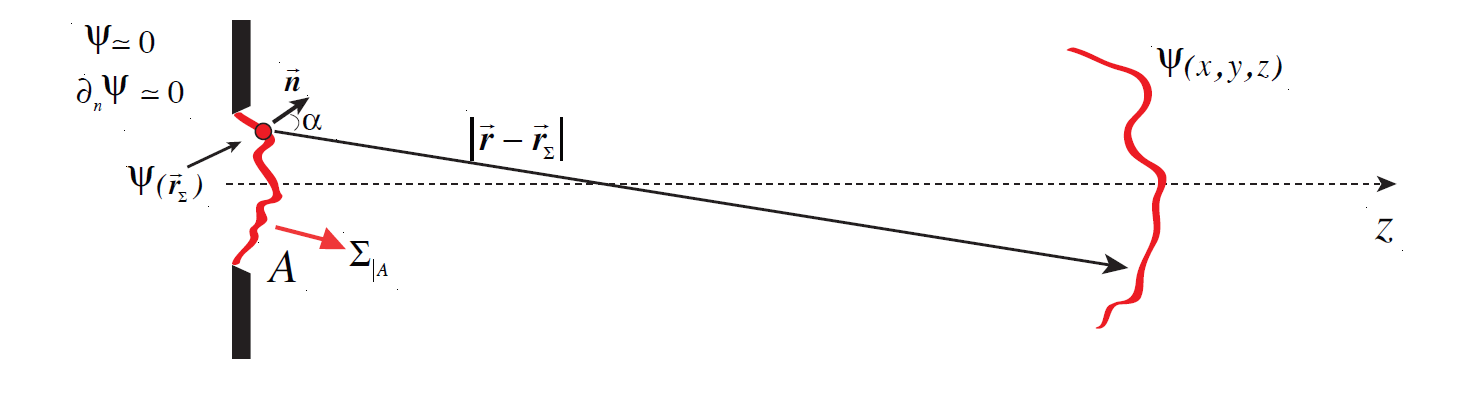
\includegraphics[scale=0.6]{05-HFY2.png}
    \caption{}
    \label{Fig:05.2-1}
\end{figure}

Finalmente existe otro factor novedoso respecto a la integral de Huygens-Fresnel: la aparición del término $-i/\lambda_0$, que tendrá gran importancia. A priori dicha integral no es trivial, y depende de la forma de $\psi(\rn_\Sigma)$ y de la forma de la superficie. Una primera aproximación de esta integral podría ser la suposición de ondas armónicas o paraxiales, con las siguientes condiciones: 

\begin{itemize}
    \item El número de onda verifica $k_0 \gg 1/r$, esto es, el punto de observación está muy alejado de la abertura. Así se podrán despreciar los términos de segundo orden de la expresión. 
    \item Tanto la función $\psi$ y $\partial_n \psi$ se toman como cero fuera de la apertura, y en la apretura toman el mismo valor que en el caso de que no hubiera tal apertura (esta es la \textit{hipótesis de Kirchoff}).
    \item La oblicuidad $\alpha$ debe de ser pequeña para que sea correcto el uso de la teoría escalar.  \\
\end{itemize}

En cuanto al factor de oblicuidad, este dependerá de la teoría seguida. Las dos más usadas son las teorías de Kirchoff y de Rayleigh-Sommerfield, cuyos factores de oblicuidad son:


\begin{equation}
    \text{Kirchoff}: \ F(\alpha) = \frac{1+\cos(\alpha)}{2} \tquad
    \text{Rayleigh-Sommerfield}: \ F(\alpha) = \cos (\alpha) 
\end{equation}
Como debe ocurrir, ambas teorías contienen la integral de Huygens-Fresnel (salvo por el factor de la longitude onda) si $\alpha\ll$, de tal modo que $F(\alpha) \approx 1$. 

\section{Analisis cualitativo: Fresnel vs Fraunhofer.}

Imaginemos que tenemos una pantalla opaca $\Sigma$, que contiene una sola apertura muy pqeueña, iluminada por ondas planas de una fuente puntual $S$ muy lejana. El plano de observación es una pantalla $\sigma$ paralela y muy cercana a $\Sigma$. En estas condiciones se proyecta sobre la pantalla una imagen de la abertura que es claramente reconocible a pesar de unas pequeñas franjas que se observan en la periferia. Si el plano de observación se aleja de $\Sigma$, la imagen de la abertura, aunque aún fácilmente reconocible, adquiere más estructura mientras que las franjas se vuelven más sobresalientes. A este fenómeno se le conoce como \textbf{difracción de Fresnel} o \textbf{difracción de campo cercano}. Si se aleja aún más el plano de observación se producirá un campo continuo en las franjas. A una gran distancia de $\Sigma$ la distribución proyectada se habrá extendido considerablemente, con lo que conservará muy poco o ningún parecido con la abertura real. En lo sucesivo, el movimiento de $\sigma$ cambia esencialmente solo el tamaño de la distribución, y no su forma. Esta es la \textbf{difracción de Fraunhofer} o \textbf{difracción de campo lejano}. Si en este punto pudiéramos reducir lo suficiente la longitud de onda de la radiación incidente, el patrón volvería al de Fresnel. Si áun se redujera más ($\lambda \rightarrow 0$), las franjas desaparecerían mientras la imagen adquiriría la forma limitadora de la abertura. como reza la óptica geométrica. Volviendo a la disposición original, si se desplazase ahora la fuente puntual hacia $\Sigma$, las ondas esféricas incidirían en la abertura para dar lugar a una distribución de Fresnel incluso en un plano de observación lejano.  \\

Así tenemos un primer indicativo de cuando podemos aplicar la difracción de Fresnel o la de Fraunhofer (que constituyen dos aproximaciones de las integrales de difracción diferentes). Siempre que la onda incidente y la onda emitida sean planas (con una diferencia de una pequeña fracción de longitud de onda) en la extensión de las aberturas difractoras (o obstáculos) se obtiene la difracción de Fraunhofer. Cuando $S$ o $P$ o las dos están demasiado cerca como para considerar despreciable la curvatura de los frentes de ondas de incidencia y de emisión prevalece la difracción de Fresnel. Como regla empírica, la difracción de Fraunhofer se producirá en una abertura/obstáculo con longitud máxima $b$ cuando 

\begin{equation}
    R>b^2/\lambda
\end{equation}
donde $R$ es la distancia más pequeña de las dos que van de $S$ hasta $\Sigma$ y de $\Sigma$ hasta $P$. Naturalmente cuando $R\rightarrow$ no importa la dimensión finita de la abertura. Asimismo, un aumento de $\lambda$ desplaza claramente el fenómeno hacia la aproximación de Fraunhofer. Cuando no podamos suponer que las ondas son paraxiales o planas tendremos que usar la integral de Huygens-Fresnel directamente.
 

\section{Difracción paraxial, conceptos y aplicaciones.}

Sea una apertura $A$ inducida en el plano $z=0$, y sean los puntos geométricas $Q=(x_0,y_0,0) \in A$ y el punto $P=(x,y,z)$ del plano de observación, de coordenadas $x,y,z$ situado a una distancia $z$ del plano la abertura, ubicado en $z=0$. Iluminando con una onda plana, tenemos que el dominio de integración es igual a la superficie plana $A$ de la abertura, que es la condición bajo la cual se ha desarrollado la teoría de la difracción fundamentada en el principio de HFY. \\ 

\begin{figure}
    \centering
    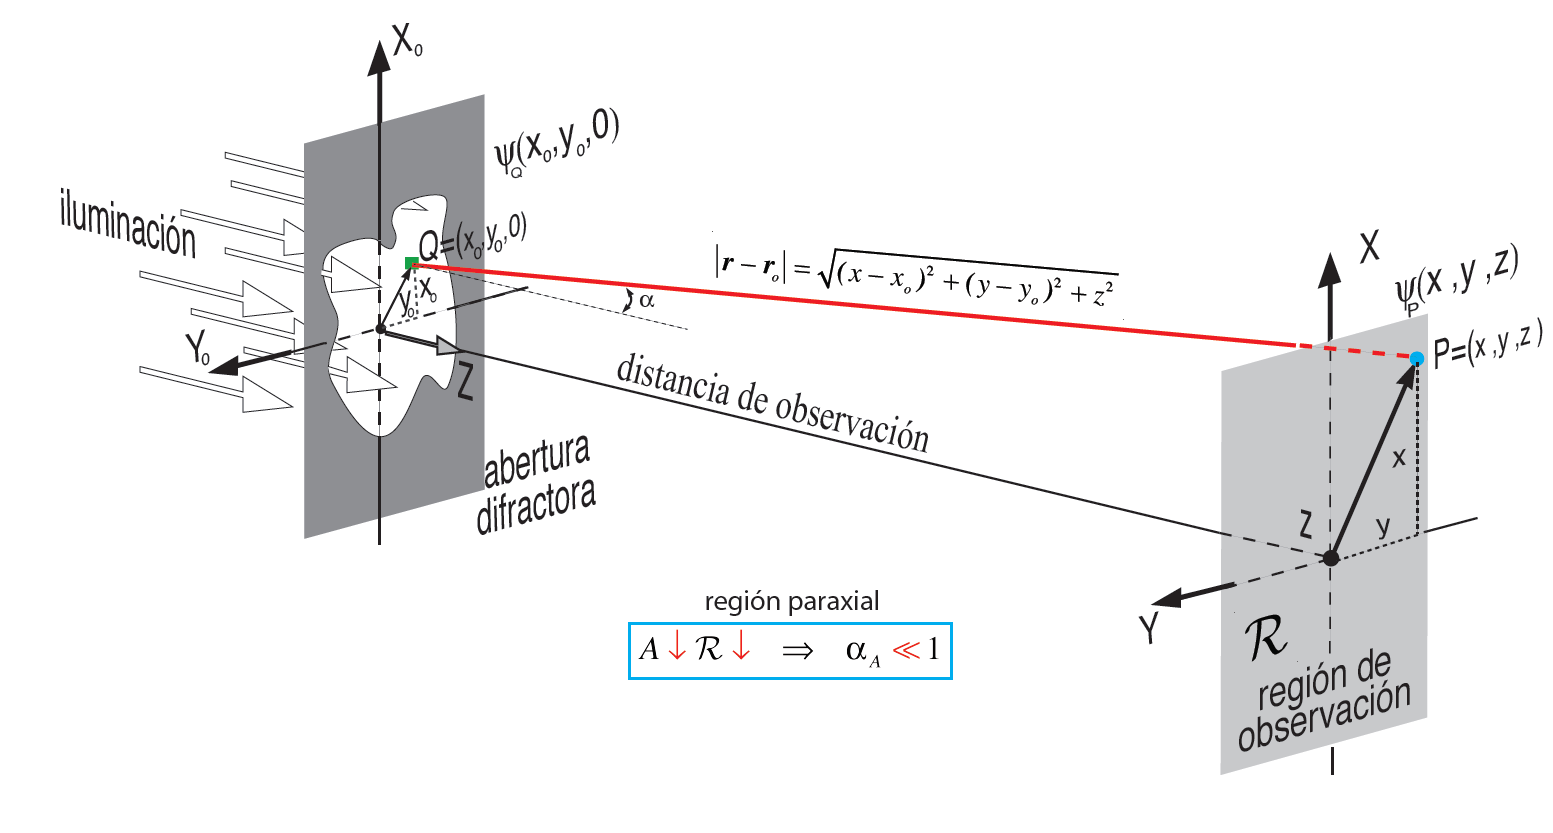
\includegraphics[scale=0.6]{05-Difraccion-1.png}
    \caption{}
    \label{Fig:05.3-1}
\end{figure}

Tenemos pues una amplitud complejo conocida $\psi\equiv\psi(x_0,y_0,0)$ y una a determinar $\psi_p \equiv \psi(x,y,z)$. Sea el módulo del vector que une ambos puntos $$|\rn-\rn_0|= \sqrt{(x-x_0)^2+(y-y_0)^2+z^2}$$ de tal modo que la \textbf{integral de difracción paraxial de Huygens-Fresnel}:

\begin{equation}
    \psi (x,y,z) \approx \frac{-i}{\lambda_0} \int_A \frac{e^{ik_0|\rn-\rn_0|}}{|\rn-\rn_0|} \psi (x_0,y_0,z_0) \D x_0 \D y_0 \label{Ec:05.03-01}
\end{equation}
Sean las condiciones, de la difracción paraxial: \\

\begin{itemize}
    \item La distancia $z$ al plano de observación es mucho mayor que las dimensiones de la abertura $A$: $|Q|\ll z$, donde $Q=(x_0,y_0)$. 
    \item La distancia $z$ del plano de observación es mucho mayor que las dimensiones de la región de observación $\mathcal{R}: \ |P|\ll z$, donde $P=(x,y)$. 
    \item De manera consistente con la hipótesis iluminación de la abertura con ondas casi planas, y de las anteriores relaciones de tamaño entre $z,A$ y $\mathcal{R}$ tenemos asegurado $\alpha \ll$, esto es, $F(\alpha)\approx 1$.
\end{itemize}

\subsection{Difracción de Fresnel}
En las condiciones de aproximación consideradas, podemos substituir la amplitud de las ondas esféricas secundarias por un valor constante en el plano de observación, pero no podemos hacer lo mismo con la distancia en la fase, allí cada pequeña variación queda amplificada por el inverso de la longitud de onda $(\lambda_0)$, por lo tanto: \\

\begin{itemize}
    \item En la amplitud $|\rn-\rn_0|\approx z$, podemos hacer una aproximación de primer orden (esto es, aproximar amplitud constante en el plano de observación):

    \begin{equation}
        \frac{1}{|\rn-\rn_0|} \approx \frac{1}{|z-z_0|} \longrightarrow \frac{1}{r} \approx \frac{1}{z}
    \end{equation}

    \item En la fase no se puede hacer esta aproximación, ya que $z$ está multiplicado por $k_0 = 2\pi / \lambda_0$, y la inversa de $\lambda$ es un valor muy grande (suponiendo el espectro visible). La fase se aproxima a primer orden, llegando así a la \textbf{aproximación parabólica de ondas esféricas} o \textbf{aproximación de Fresnel}:

    \begin{equation}
        \frac{e^{ik_0|\rn-\rn_0|}}{|\rn-\rn_0|} \longrightarrow \frac{1}{z} e^{ik_0z} e^{\frac{ik_0}{2z} \ccorchetes{(x-x_0)^2+(y-y_0)^2}}
    \end{equation}
\end{itemize}

Por tanto la integral de difracción en esta aproximación, es la \textbf{integral de difracción de Fresnel}: 

\begin{equation}
    \psi (x,y,z) \approx \frac{-ie^{ik_0z}}{\lambda_0 z} \int_A \psi (x_0,y_0,0) e^{\frac{ik_0}{2z}\ccorchetes{(x-x_0)^2+(y-y_0)^2}} \D x_0 \D y_0
    \label{Ec:05.3-04}
\end{equation}
que podremos escribir de manera alternativa

\begin{equation}
    \psi (x,y,z) = \int_{\mathbb{R}^2} \psi (x_0,y_0) K(x,y,x_0,y_0,z) \D x_0 \D y_0
\end{equation}
donde hemos usado el denominado \textbf{Kernel} (también llamado \textbf{función de Green} o \textbf{propagador}) de la difracción de Fresnel:

\begin{equation}
    K(x,y,x_0,y_0,z) = \frac{-ie^{ik_0z}}{\lambda_0 z} e^{\frac{ik_0}{2z} \ccorchetes{(x-x_0)^2+(y-y_0)^2}}
\end{equation}

\subsection{Difracción de Fraunhofer}

El Kernel de Fresnel tiene un factor de fase cuadrática en las variables del plano de la abertura $A$ (que son $(x_0,y_0,z_0)$). Tal y como hemos visto en el análisis cualitativo, la difracción de Fraunhofer aparece cuando ambas el plano de incidencia está suficientemente lejos de la abertura, y por tanto $x_0^2$ e $y_0^2$ son despreciables frente a $z$. Entonces desarrollando estos términos podemos ver que 

\begin{equation}
\begin{array}{rll}
    K(x,y,x_0,y_0,z) &  = &  \frac{-i e^{ik_0z}}{\lambda_0 z} e^{\frac{ik_0}{2z} \ccorchetes{(x-x_0)^2+(y-y_0)^2}} \\ \\ & = & \frac{-i e^{ik_0z}}{\lambda_0 z}
     e^{\frac{ik_0}{2z} \ccorchetes{x^2+2xx_0+x_0^2+y^2+2yy_0+y_0^2}}    
\end{array}
\end{equation}
Por lo que la condición para que tengamos la \textbf{difracción de Fraunhofer} ocurre cuando:

\begin{equation}
     e^{\frac{ik_0}{2z} \ccorchetes{x_0^2+y_0^2}}   \approx 1  
\end{equation}
que se puede conseguir aumentando la separación $z$ entre el \textit{plano abertura-plano observación}, o aumentando la longitud de onda:

\begin{equation}
    z \gg \frac{k_0}{2} (x_0^2 + y_0^2)_{\max}
\end{equation}
Si ocurre esto nuestra fase podremos expresar la fase como

\begin{equation}
    \varphi \approx k_0 z + \frac{k_0}{2z} \ccorchetes{(x^2+y^2)-2(xx_0+yy_0)} = k_0z + \frac{k_0}{2z} \ccorchetes{(x^2+y^2)- 2 \pi (f_xx_0+f_yy_0)}
\end{equation}
donde hemos introducido las \textbf{frecuencias espaciales ópticas} (número de onda dividido entre $2\pi$):

\begin{equation}
    f_x = \frac{xK_0}{z2\pi} = \frac{k_x}{2\pi} \tquad f_y = \frac{yk_0}{z 2 \pi} = \frac{k_y}{2\pi}
\end{equation}
por tanto la \textbf{integral de Fraunhofer} queda como

\begin{equation}
    \psi (x,y,z) \approx \mathcal{E}_0 (x,y,z) \int_A \psi (x_0,y_0,0) e^{i2\pi [f_x x_0 + f_y y_0]} \D x_0 \D y_0 \label{Ec:05.04-12}
\end{equation}
donde $\mathcal{E}_0 (x,y,z) = \frac{-ie^{ik_0z}}{z \lambda_0}e^{\frac{ik_0}{2z}(x^2+y^2)}$. Si nos damos cuenta el término integral es una trasformada de Fourier de la función $\psi(x_0,y_0)$. La denotaremos por $\TF(\psi(x_0,y_0))$. Cabe destacar que la aproximación de Fraunhofer se vuelve exacta cuando $z\rightarrow \infty$. En el siguiente apartado veremos como implementar el infinito, de tal forma que la aproximación de Fraunhofer deje de ser una aproximación.

\subsection{Difracción de Fraunhofer con lente}

Una lente es, como ya hemos visto, un elemento óptico que nos permite \textit{traer el infinito al plano local}. En este plano, como veremos es posible obtener la \textit{transformada de Fourier} exacta de la amplitud incidente en la apertura. Coloquemos la lente (a priori de tamaño infinito) en el plano de abertura (plano de coordenadas), iluminada por un frente de onda plano, monocromática y de amplitud unidad. En ese caso la función de trasmisión solo altera la fase:

\begin{equation}
    \psi (x_0,y_0) = t_L (x_0,y_0) t_A (x_0,y_0) \psi (x_0,y_0,0)
\end{equation}
El cálculo de la difracción producida por esta lente implica usar la integral de difracción de Fresnel (ecuación \ref{Ec:05.3-04}) de la función de ondas anterior (onda plana monocromática multiplicadad por las funciones de trasmisión) en el plano $z=f$. Debido al efecto de la lente tenemos que el término cuadrático $e^{i\frac{k_0}{2z}\ccorchetes{(x-x_0)^2+(y-y_0)^2}}$ se anula (ya que en $z=f$ tendríamos que ambos son iguales con signos distintos). En ese caso la fase de Fraunhofer dejaría de ser una aproximación y pasaría a ser una integral exacta, tal que:

\begin{equation}
    \psi (x,y,f) = \mathcal{E}_0 (x,y,f) \int_{\mathbb{R}^2} \psi (x_0,y_0,0) e^{-i k_0 \ccorchetes{\frac{x}{f}x_0+\frac{y}{f}y_0}} \D x_0 \D y_0
\end{equation}
Esta integral es una delta de dirac ya que solo adquiere valores cuando $k_0x/f=0$, de tal modo que

\begin{equation}
    \intinf e^{- i 2 \pi (p-p')q} \D q = \delta (p-p') \tquad \delta (xa) = \frac{1}{|a|} 
\end{equation}
por lo que:

\begin{equation}
    \psi (x,y,f) = \frac{-i}{\lambda_0f} e^{ik_0f}\delta \parentesis{\frac{k_0x}{f},\frac{k_0y}{f}} = - i \lambda_0 f e^{ik_0f} \delta(x,y)
\end{equation}
Por tanto la onda difractada por una lente (de dimensiones infinitas) en el plano focal es una delta de Dirac en el eje, esto es, la transformada de Fourier de una onda plana. De haber considerado una lente finita, dejaremos de observar un punto luminoso en el plano focal. Este se ensanchará transversalmente y dará lugar a una PSF (Point Spread Function), esto es, un patrón de anillos cada vez mas tenues, con un máximo en el centro (como si fuera un $\sinc (\rho)$ en el plano de observación).

\subsection{Difracción de Fraunhofer de una abertura reducida entorno al origen}

Ahora se llevará a cabo una aproximación distinta de la expresión de la difracción de Fraunhofer, empleando como variables espaciales para el desarrollo, la distancia entre el origen (0,0,0) y el punto del plano de observación (x,y,z). En ese caso:

\begin{equation}
    R = x^2 + y^2 + z^2 = |\rn|^2 \tquad R_0^2 = x_0^2 + y_0^2 = |\rn_0|^2
\end{equation}
Suponiendo la aproximación paraxial:

\begin{equation}
    |\rn-\rn_0|\approx R - \frac{\rn \cdot \rn_0}{R} \tquad \frac{1}{|\rn-\rn_0|} \approx \frac{1}{R} \parentesis{1+\frac{\rn \cdot \rn_0}{R^2}}
\end{equation} 
Substituyendo en la ecuación \ref{Ec:05.03-01} tenemos que:

\begin{eqnarray}
    \psi (R) &  = &  - \frac{i}{\lambda_0} \frac{e^{ik_0R}}{R} \int \psi(\rn_0) e^{-ik_0\frac{\rn \cdot \rn_0}{R}} \D \rn_0  \\ & \approx &  - \frac{i}{\lambda_0} \frac{e^{ik_0R}}{R} \int \psi (\rn_0) e^{-ik_0\frac{x}{R}x_0}e^{-ik_0\frac{y}{R}y_0} \D x_0 \D y_0
\end{eqnarray}
Si nombranos $\sin(\alpha) = x/R$ y $\sin(\beta)=y/R$ llegamos a que

\begin{equation}
    \psi (R) = - \frac{i}{\lambda_0} \frac{e^{ik_0R}}{R} \int \psi (\rn_0) e^{-ik_0\sin(\alpha) x_0}e^{-ik_0\sin(\beta) y_0} \D x_0 \D y_0
\end{equation}
En el $R\gg R_0$ la expresión de la fase del Kernel queda en términos del $\sin(\alpha)$ y del $\sin (\beta)$ que no están restringidos a la zona paraxial en la que debería cumplirse que $\sin(\alpha)\sim \alpha$ y $\sin(\beta)\sim \beta$; por lo que ahora se obtiene una trasnformada de Fourier de la onda incidente que es válida en un rango angular mayor que el del rango paraxial. Esto permite explicar que el patrón de difracción cristalino producido por los rayos $X$ se pueda observar en rangos angulares mucho mayores que la limitada zona paraxial.  

\section{Principio de Babinet}

El \textbf{principio de Babitet} afirma que detrás de un obstáculo opaco habrá zonas de intensidad no nula debido a que la difracción de Fresnel producida por su apertura complementaria en general tiene un valor distinto a cero. Este principio se basa en la hipótesis de difracción de Kirchoff, por lo que su rango de validez está limitado a la aproximación paraxial. La expresión matemática de este principio es:

\begin{eqnarray}
    \psi (x,y,z) = \psi_A(x,y,z)+\psi_{\bar{A}} (x,y,z) 
\end{eqnarray}
donde $\psi$ es la expresión de la onda si no hubiera obstáculo. De esta forma podemos calcular la amplitud compleja difractada por un obstáculo $\bar{A}$ a partir de de la difractada por la apertura complementaria. \\

En la aproximación de Fraunhofer sabemos que $\psi(x,y,z) = \mathcal{P}(x,y)$ donde esta función $\mathcal{P}(x,y)$ es una función muy estrecha (idealmente una delta de Dirac). Entonces el campo difractado sin obstáculo es prácticamente nulo en todo el espacio salvo en un intervalo muy pequeño alrededor de (0,0). Una buena aproximación es, em este caso:

\begin{equation}
    \psi_{\bar{A}} (x,y,z) \approx - \psi_A(x,y,z) \tquad \forall (x,y) \neq (0,0)
\end{equation}

\begin{figure}[h!]
    \centering
    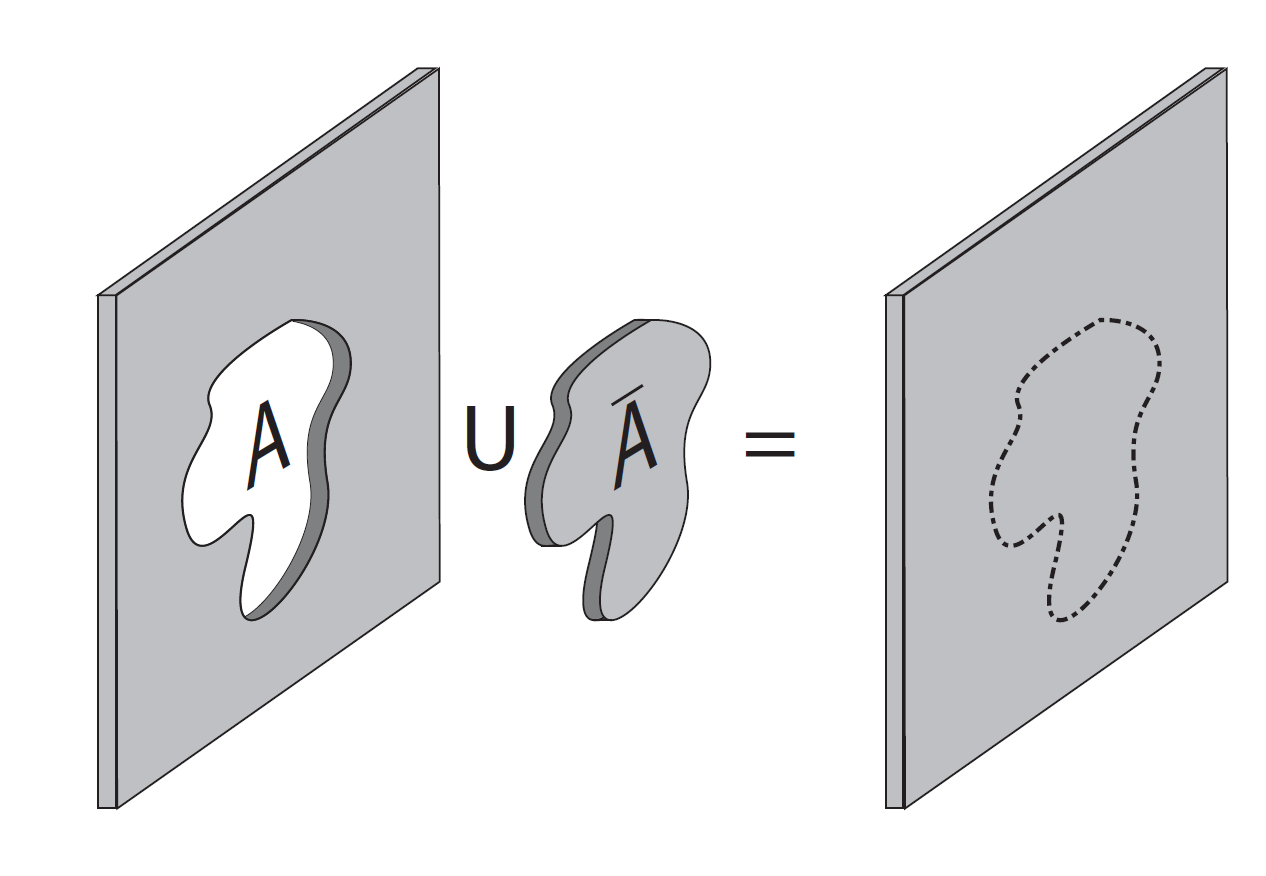
\includegraphics[scale=0.3]{05-Babinet.png}
    \caption{}
    \label{Fig:05.03}
\end{figure}


\section{Teoría de difracción coherente de la imagen}



\subsection{Imagen de un punto: respuesta de impulso.}

Consideremos tres planos para formalizar matemáticamente la teoría difraccional coherente de la imagen: el plano objeto, con coordenadas $(x_0,y_0,-z_1)$; el plano lente $(x_L,y_L,0)$ y el plano imagen $(x,y,+z_2)$. Sea una fuente puntual $S$ situada el plano objeto en las posiciones ($x_s,y_s,-z_1$), que genera odnas esféricas de amplitud unidad. Teniendo en cuenta la expresión de la difracción de Fresnel (ecuación \ref{Ec:05.3-04}) y las correspondientes ecuaciones de trasmisión (lente), podemos ver que:

\begin{equation}
    \psi (x,y,z) = \frac{e^{ik_0(-z_1+z_2)}}{\lambda_0^2 z_1 z_2} e^{-i \frac{k_0}{2z_1} (x_0^2 + y_0^2)} e^{i \frac{k_0}{2z_2}(x^2+y^2)} \delta \parentesis{-\frac{x}{\lambda z_2}+\frac{x_0}{\lambda z_1}, \frac{-y}{\lambda z_2} + \frac{y_0}{\lambda z_1}}
\end{equation}
de tal modo que el Kernel:

\begin{equation}
    K(x,y,x_0,y_0,z_2) = \frac{e^{ik_0(-z_1+z_2)}}{M} e^{-i\frac{k_0}{2z_1} (x_0^2+y_0^2)} e^{i \frac{k_0}{2z_2}(x^2+y^2)} \delta\parentesis{-\frac{x}{M}+x_0, - \frac{y}{M}+y_0} \label{Ec:05.4-02}
\end{equation}
Esta ecuación \ref{Ec:05.4-02} es conocida la llamada \textbf{respuesta impulso del sistema} (PDF o Kernel), y nos da la amplitud compleja producida por un punto luminoso arbitrario en el plano imagen de una lente. Lógicamente podemos extenderla a una distribución de amplitud de objeto arbitraria (esto es, un objeto extenso), de tal modo que:

\begin{equation}
    \psi (x,y,z_2) = \int t(x_0,y_0) K (x,y,x_0,y_0,z_2) \D x_0 \D y_0 
\end{equation}
aplicando la delta de Dirac para relacionar $x_0$ e $y_0$ con $x$ e $y$, obteniendo así:

\begin{equation}
    \psi (x,y,z_2) = \frac{e^{ik_0 (-z_1+z_2)}}{M} e^{\frac{ik_0}{2z_2} \parentesis{1-\frac{1}{M}}(x^2+y^2)} t\parentesis{\frac{x}{M},\frac{y}{M}}
\end{equation}
obteniendo una réplica exacta de la amplitud del objeto salvo fases y un factor de escala.

\subsection{Imagen de un punto: función PSF}

En el caso anterior hemos considerado que el Kernel tenía como dominio de integración era $\mathbb{R}^2$, por lo que la respuesta de impulsos del sistema es de anchura nula. Sin embargo si consideramos una situación realista, como puede ser una lente de abertura finita, tendremos que la PSF de anchura nula (delta de Dirac) se convertirá en una PSF de anchura finita. Denotaremos por $D$ a la función PSF de anchura finita, tal que:

\begin{equation}
    K(x,y,x_0,y_0,z_2)=\frac{e^{ik_0(-z_1+z_2)}}{M} e^{-\frac{ik_0}{2z_1}(x_0^2+y_0^2)} e^{-i\frac{k_0}{2z_2}(x^2+y^2)} D\parentesis{-\frac{x}{M}+x_0,-\frac{y}{M}+y_0}
\end{equation}
donde la función $D\parentesis{-\frac{x}{M}+x_0,-\frac{y}{M}+y_0}$ viene dada por:

\begin{equation}
    D\parentesis{-\frac{x}{M}+x_0,-\frac{y}{M}+y_0} = \frac{1}{\lambda_0^2z_1^2} \int_A e^{ik_0\ccorchetes{\frac{1}{z_1}\parentesis{-\frac{x}{M}+x_0} + \frac{1}{z_1}\parentesis{-\frac{y}{M}+y_0}}} \D x_L \D y_L
\end{equation}
Esta integral es la transformada de Fourier de la abertura de la lente, excepto por el desplazamiento (si tomáramos $x_0=y_0=0$ obtendríamos la transformada). De este  resultado se concluye que $\mathcal{P}=|K|^2$ es una función de dimensiones no nula, e invariante frente a desplazamientos. En general es una función tipo campana que tiende a $\delta$ cuando $A \rightarrow \infty$. También se puede comprobar que si $\lambda_0 \rightarrow 0$ volvemos al límite geométrico: la imagen de un punto es otro punto. Se comprueba, por otra parte, que aproximadamente una fase cuadrática en $(x_0,y_0)$ se conecta con una fase cuadrática en el plano imagen, usando el aumento $M$. Consecuentemente la imagen de un objeto compuesto por un número arbitrario de fuentes puntuales distribuidas irregularmente (de acuerdo con su función de trasmisión) por la superficie del plano objeto, será dada por: 

\begin{equation}
    \psi (x,y,z_2) = \frac{e^{ik_0(-z_1+z_2)}}{M} e^{-\frac{ik_0}{2z_1}\parentesis{1-\frac{1}{M}}(x^2+y^2)} \int t(x_0,y_0) D(x,y,x_0,y_0) \D x_0 \D y_0 
\end{equation}
La amplitud compleja imagen de un objeto arbitario entonces se obtendrá a partir de la convolucuión de la amplitud de entrada de la PSF del sistema:

\begin{equation}
    \psi (x,y,z_2) = t(x_0,y_0) * K (x-\eta_0,y-\gamma_0)
\end{equation}

\subsection{Transformada de Fourier y Teoría de Abbe}

La \textbf{teoría difraccional de la imagen} desarrollada por E. Abbe, también llamada \textbf{teoería de Abbe}, consiste en considerar el proceso de formación de la imagen como un proceso de dos etapas o de doble difracción. \\

Primero se produce la transformada de Fourier por difracción de Fraunhofer en el plano focal de la imagen de la lente, donde obtenemos una \textit{distribución espectral} (o distribución de Fourier); mientras que en la segunda etapa se obtiene por medio de una difracción de Fresnel una distribución proporcional a la transformada de Fourier de la primera trasformada de Fourier, que por consistencia es una transformada de fourier inversa:

\begin{equation}
    \psi (x,y,z_2) = \mathrm{TF}^{-1} (\mathrm{TF}(\psi(x_0,y,z=0)))
\end{equation}

Esta nueva perspectiva tiene consecuencias físicas muy relevantes en el tratamiento y procesado óptico de la información, formación de imagen en microscopía, filtrado espacial, computación lógica y digital...

\chapter{Difracción de Fresnel}

En este tema vamos a saber describir y formalizar problemas canónicos de difracción en zona de Fresnel, destacando sus efectos sobresalientes, así como calcular campos ópticos difractados en regiones de gran valor conceptual (especialmente a lo largo del eje óptico) posibilitando un análisis del proceso difraccional en base a argumentos interferenciales. También aprenderemos a aplicar los conceptos y destrezas adquiridas en el estudio de elementos ópticos difractivos, centrándonos en las placas zonales de amplitud y fase (entendidas como lentes difractivas multifocales). En base a los conocimientos de difracción e interferencia, se introducirán los conceptos básicos de la holografía como técnica de registro y almacenamiento de información de objetos tridimensionales. \\

\section{Estudio canónico (integral)}


Hasta ahora hemos considerado dispositivos y ondas planas de \textit{extensión infinita} para poder usar las integrales impropias (de límites infinitos) tabuladas, obteniendo un análisis de las implicaciones físicas del fenómeno difractivo mas sencillo. Para poder tener un modelo mas realista vamos a tener que estudiar objetos ahora con dimensiones finitas. \\

\subsection{Semiplano: análisis asintótico}

Consideremos la situación más simple posible: la que se produce en un borde de un semiplano óptico cuando se ilumina con una onda plana de amplitud unidad, propagándose en el eje $z$. En este caso la \textit{función de trasmisión}


\begin{equation}
    t(x_0,y_0) = \left\lbrace \begin{array}{ll}
       1  & x_0>0 \ \forall y_0  \\
       0  & x_0\leq 0 \ \forall y_0
    \end{array} \right.
\end{equation}
La óptica geométrica predice que a partir del borde hay un cambio abrupto de iluminación pasando de una intensidad nula a una no nula constante. Sin embargo lo que se observa es una distribución de intensidad variada, con franjas de diferentes grosores y frecuencia variable. \\

Evaluamos la intensidad observada en la coordenada $x=0$. Calculando la amplitud difractada por el borde situado en $x_0=0$:

\begin{equation}
    \psi (x=0,y,z) = \frac{-i e^{ik_0z}}{\lambda_0 z} \int_0^\infty \intinf  +
    e^{\frac{ik_0}{2z} \ccorchetes{(-x_0)^2+(y-y_0)^2}}  \D x_0 \D y_0
\end{equation}
utilizando la integral gaussiana

\begin{equation}
    \intinf e^{at^2+bt} \D t  = \sqrt{\frac{\pi}{-a}} e^{-b^2/4a}
\end{equation}
llegando a que la onda en $x=0$:

\begin{equation}
    \psi (x=0,y,z) = \frac{1}{2} e^{ik_0z}
\end{equation}
por lo que la intensidad es $I=|\psi|^2=1/4$. El cálculo de la intensidad en otros puntos del plano de observación, no sólo del borde de la teórica sobra geométrica, sino en la zona que según la teoría geométrica tendría intensidad constante, se puede realizar de forma más directa con la teoría desarrollada por Rubinowicz. Esta teoría establece que las oscilaciones debidas a la difracción por borde se obtiene como superposición de las ondas planas que se propagan en la zona libre con ondas cilíndricas difractadas por el borde. \\

\begin{figure}[h!]
    \centering
    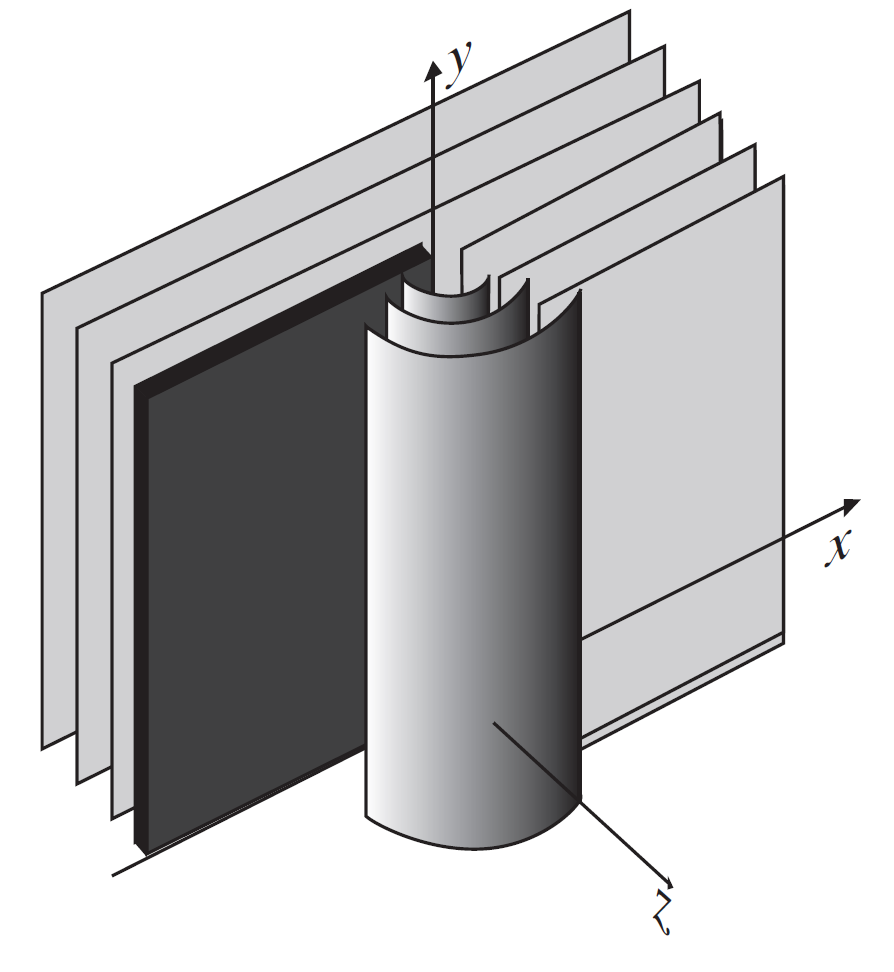
\includegraphics[scale=0.5]{06-Cilindricas.png}
    \label{Fig:06.01-01}
    \caption{}
\end{figure}


Estas ondas cilíndricas se pueden explicar usando el principio de Huygens, en el cual cada punto es un emisor de ondas esféricas y la envolvente de estas reconstruye el frente de onda cilíndricas. EN ese caso la onda difractada en el plano de observación será:

\begin{equation}
    \psi (x,y,z) = \psi_0 e^{ik_0z} + \frac{\psi_b}{\sqrt{\rho}} e^{ik_0 \rho}
\end{equation}
de tal modo que en aproximación paraxial $\rho \approx z + \frac{1}{2} \frac{x^2}{z}$:

\begin{equation}
    \psi (x,y,z) = \psi_0 e^{ik_0z} + \frac{\psi_b}{\sqrt{\rho}} e^{ik_0Z} e^{ik_0 \frac{x^2}{2z}}
\end{equation}
de tal modo que la intensidad resultante viene dada por

\begin{equation}
    I = |\psi_0|^2 + \frac{|\psi|^2}{\rho} + \frac{2}{\sqrt{\rho}} |\psi_0||\psi_b|\cos (k_0x^2/2z)
\end{equation}

\subsection{Difracción en una abertura cuadrada}

La segunda estructura difractora a considerar es una abertura cuadrada de dimensiones 2a x 2a. Se ilumina la abertura con ondas esféricas de amplitud compleja $\psi_0$, provenientes de una fuente puntual situada en la posición $z=-L$. Es importante para la resolución del problema, tal como veremos más adelante, conocer la posición de la abertura con respecto al eje óptico (es decir la posición de los vértices $x_{01}$ y $x_{02}$ en el eje $x_0$ y los vértices $y_{01}$ y $y_{02}$ en el eje $y_0$) del plano de la abertura, que está situado en la posición axial $z=0$. \\

En la aproximación de Fresnel de la integral de Kirchoff la amplitud de la onda difractada en el punto central $P=(0,0,z)$ de coordenadas:

\begin{equation}
    \psi (P) = \frac{-ie^{ik_0z}}{\lambda_0 z} \int_{x_{01}}^{x_{02}} \int_{y_{01}}^{y_{02}} \psi_0 (x_0,y_0,0) e^{\frac{ik_0}{2z}\ccorchetes{(0-x_0)^2+(0-y_0)^2}} \D x_0 \D y_0 
\end{equation}
Considerando la onda esférica de amplitud unidad

\begin{eqnarray}
    \psi_0 (x_0,y_0,0) = \frac{e^{ik_0L}}{L} e^{i\frac{k_0}{2L}\parentesis{x_0^2+y_0^2}}
\end{eqnarray}
de tal modo que la onda difractada en $P$ es

\begin{equation}
    \psi (P)= \frac{-i^{ik_0(z+L)}}{\lambda_0 z L}\int_{x_{01}}^{x_{02}} \int_{y{01}}^{y_{02}} e^{i\frac{k_0}{2L}\parentesis{x_0^2+y_0^2}\parentesis{\frac{1}{L}+\frac{1}{z}}} \D x_0 \D y_0
\end{equation}
haciendo el cambio de variables 

\begin{equation}
    u = x_0 \sqrt{\frac{2}{\lambda_0} \parentesis{\frac{1}{L} + \frac{1}{z}}}  \tquad v = y_0 \sqrt{\frac{2}{\lambda_0} \parentesis{\frac{1}{L}+\frac{1}{z}}}
\end{equation}
Este cambio de variables es un reescalado de las dimensiones, pero que facilitará mucho la integración. En este caso tendremos que


\begin{equation}
    \psi (0,0,z) = \frac{-ie^{ik_0(z+L)}}{\lambda_0 z L} \ccorchetes{\frac{2}{\lambda_0} \parentesis{\frac{1}{L} + \frac{1}{z}}}^{-1} \int_{u_1}^{u_2} e^{i\frac{\pi}{2}u} \D u \int_{v_1}^{v_2}e^{i\frac{\pi}{2}v} \D v
\end{equation}
Estas integrales están tabuladas en las conocidas \textit{integrales de Fresnel}, que simplifican de sobremanera el cálculo. En ese caso tenemos que:

\begin{equation}
     \Ccal (\omega) = \int_0^\omega \cos (\pi \tilde{\omega}/2) \D \tilde{\omega} \tquad     \Scal (\omega) = \int_0^\omega \sin (\pi \tilde{\omega}/2) \D \tilde{\omega}
\end{equation}
De este modo tenemos que

\begin{equation}
    \psi (0,0,z) = \frac{E_0}{2} \ccorchetes{\Ccal (u) + i\Scal (u)}_{u_1}^{u_2} \ccorchetes{\Ccal (v) + i \Scal (v)}_{v_1}^{v_2}
\end{equation}
Dada la simetría de las funciones $\Scal(\omega)=-\Scal(-\omega)$ y $\Ccal(\omega)=\Ccal(-\omega)$ es posible reducir el tamaño del resultado. 

\subsection{Semiplano: análisis de Cornú}

Cuando consideramos $x_1,x_2,y_2 \rightarrow \infty$ estamos convirtiendo nuestra apertura rectangular en un semiplano. Dado que se verifica que $\Ccal (\infty) = \Scal (\infty) = 1/2$, tenemos que en este caso se verifica que:

\begin{equation}
    I_P = \frac{I_0}{2} \ccorchetes{\parentesis{\frac{1}{2}-\Ccal(v_1)}^2+\parentesis{\frac{1}{2}-\Scal(v_1)}^2}
\end{equation}
Para $y_{01}=0$, como $\Ccal(0)=0$ y $\Scal(0)=0$, tenemos que $I_P=I_0/4$, recuperando el resultado por el análisis asintótico. Al elegir un valor de las coordenadas espaciales concreto, se debe considerar ahí el punto $P$ del cálculo anterior, y estimar el desplazamiento que debe hacerse con el borde $y_{01}$ hacia arriba o hacia abajo (es decir, debemos hacer un cambio de coordenadas). Así obtendremos en ese punto región la intensidad resultante. En función del desplazamiento de $y_1$ (o de $v_1$) considerado respecto a $P$, obtenemos una intensidad u otra (figura \ref{Fig:06.1-03}).

\begin{figure}[h!]
    \centering
    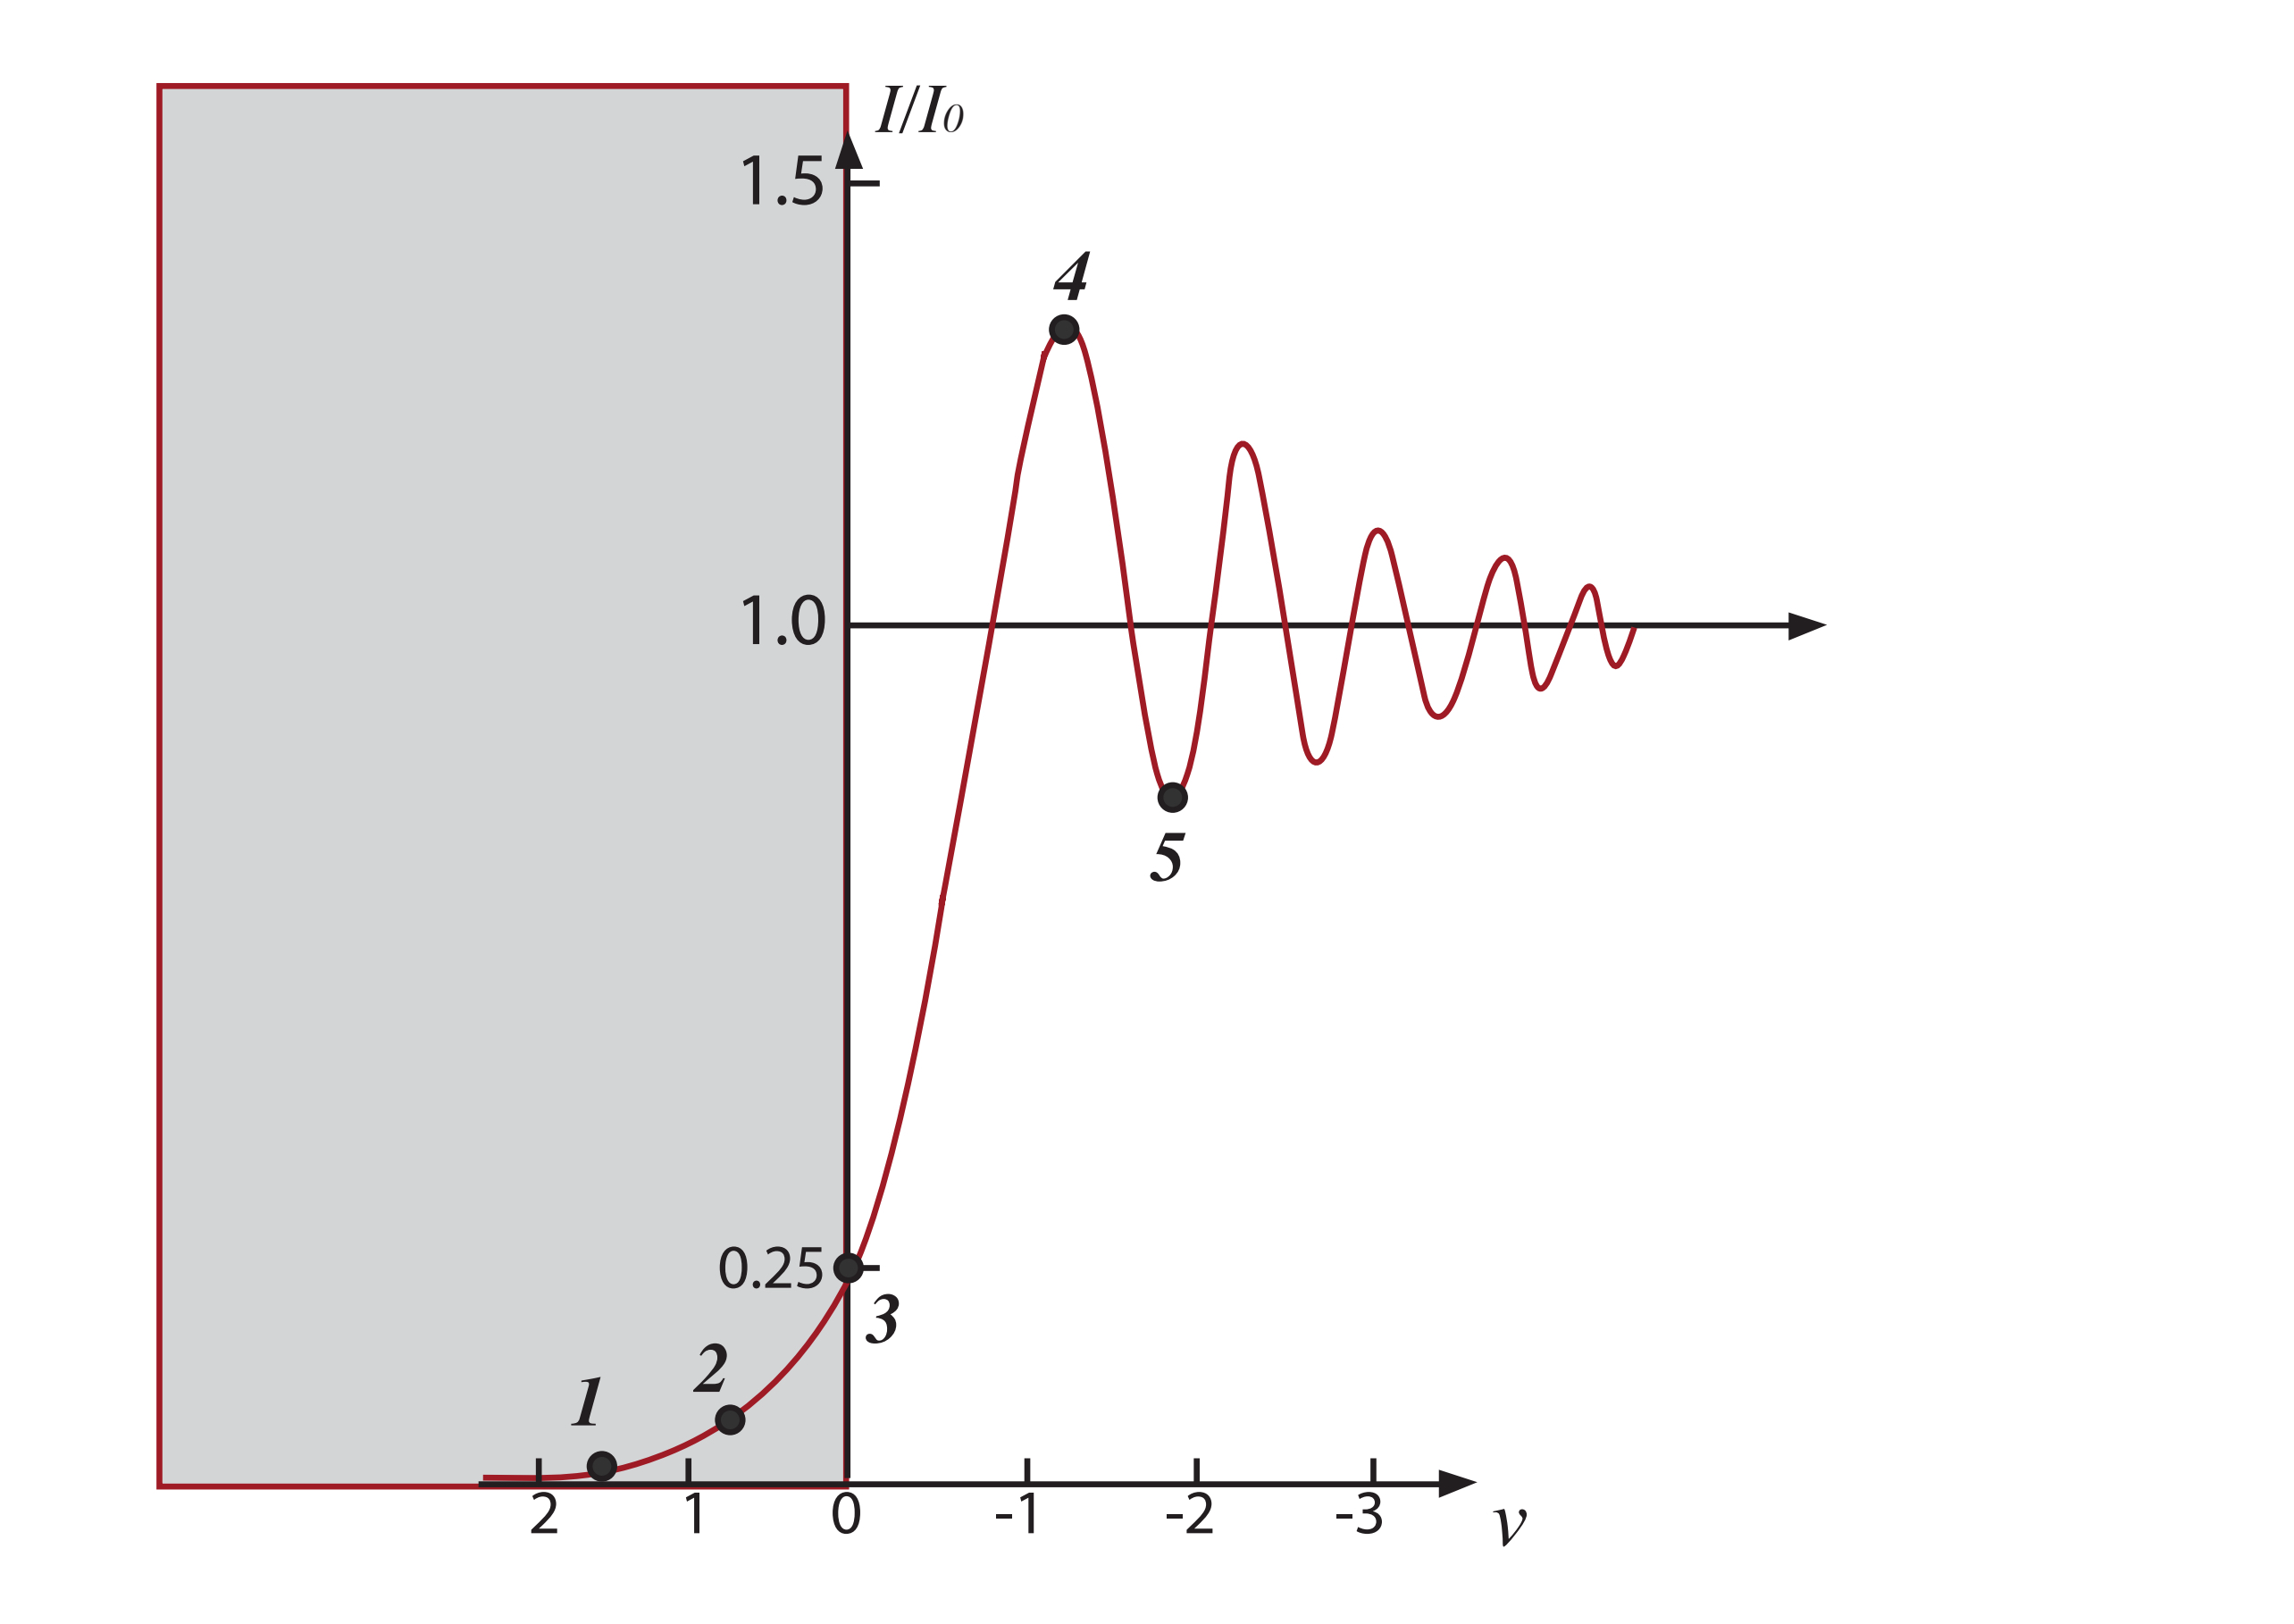
\includegraphics[scale=0.1]{06-Semiinfinito.png}
    \caption{}
    \label{Fig:06.1-03}
\end{figure}

\section{Difracción de Fresnel en el eje}

\subsection{Apertura circular}

\begin{figure}[h!]
    \centering
    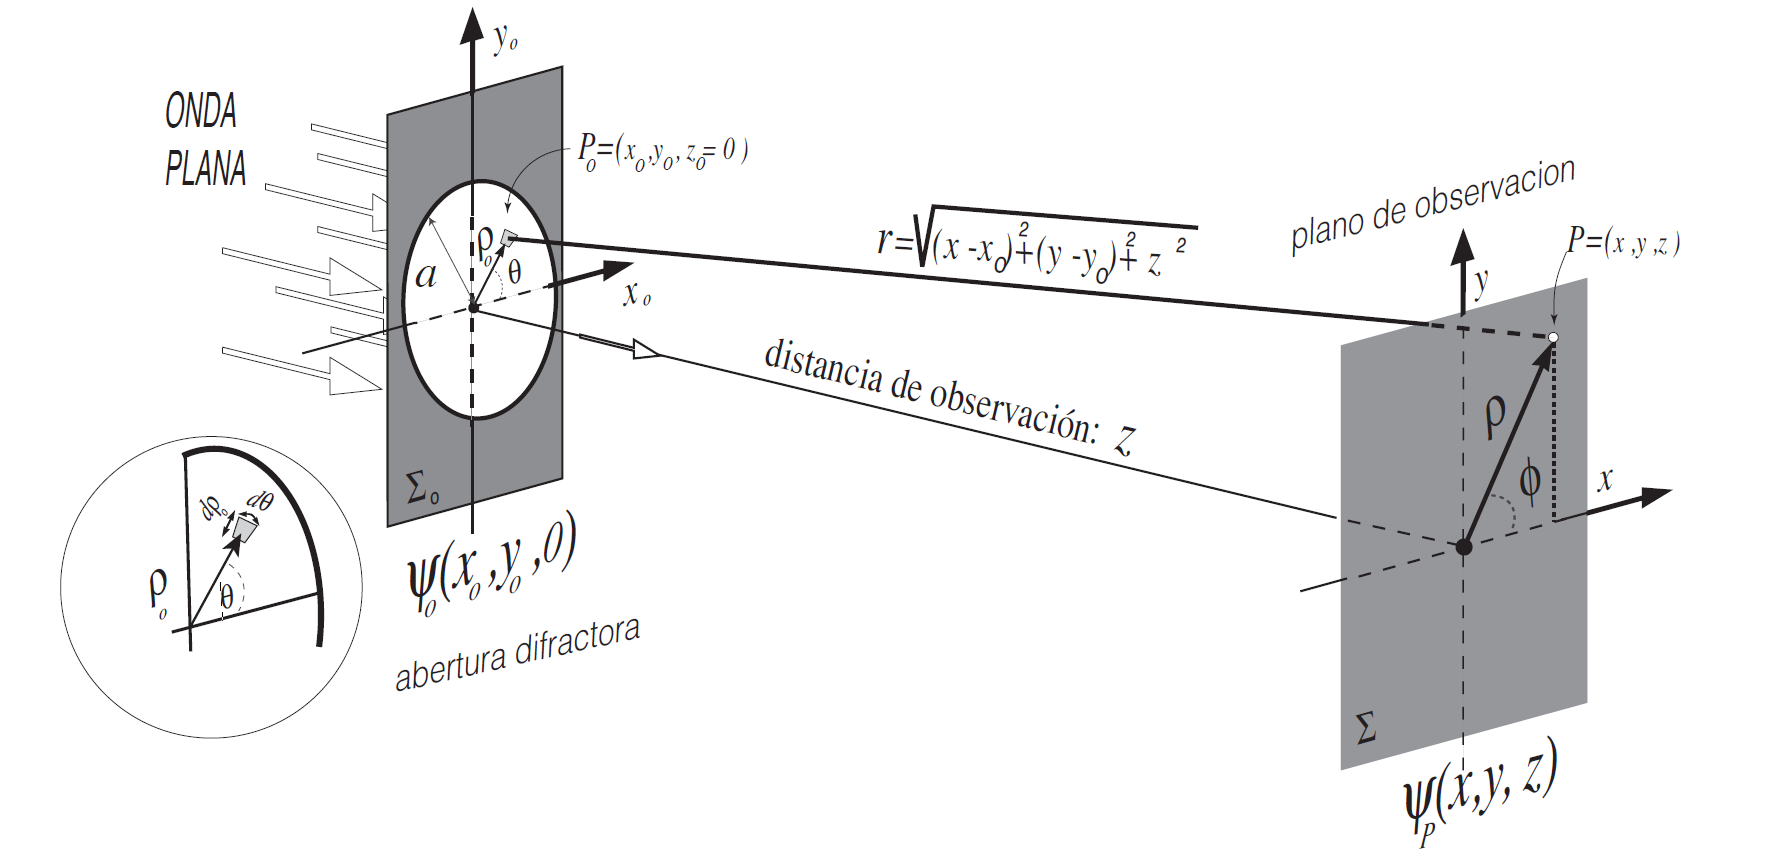
\includegraphics[scale=0.5]{06-Circular.png}
    \label{Fig:06.1-02}
\end{figure}

Consideremos la difracción de Fresnel en aberturas de simetría circular de radio $a$ e iluminadas con una onda plana. En esta sección trabajaremos en coordenadas polares. La difracción de Fresnel en el punto $P=(x=0,y=0,z)$

\begin{eqnarray}
    \psi_P (\rho=0,z) &  =   & \frac{-ie^{ik_0}}{\lambda_0z} \int_0^{2\pi} \int_0^a e^{\frac{ik_0}{2z} \rho^2_0} \rho_0^2 \D \rho_0 \D \theta \\&  =  &  -e^{ik_0z} \ccorchetes{e^{\frac{ik_0}{2z}\rho^2_0}}_0^a = - e^{ik_0z }\ccorchetes{e^{\frac{ik_0}{2z}a^2}-1}
\end{eqnarray}
de tal modo que la intensidad viene dada por

\begin{equation}
    I(0,z) = 2 \ccorchetes{1-\cos \parentesis{\frac{\pi a^2}{\lambda_0 z}}} = 4 \sin^2 \parentesis{\frac{\pi a^2}{2 \lambda_0 z}}
\end{equation}
Los máximos y los mínimos de intensidad se obtienen en los puntos de coordenada $z$:

\begin{equation}
  \mathrm{Maximos}: \  \frac{\pi a^2}{2\lambda_0z} = \frac{(2m+1)\pi}{2} \tquad 
  \mathrm{Minimos}: \  \frac{\pi a^2}{2\lambda_0z} = m \pi
\end{equation}
aunque en el límite $z\rightarrow \infty$, tenemos que $I\rightarrow 0$. 


\subsection{Difracción de fresnel por obstáculo circular}

Ante la dificultad de calcular analíticamente la difracción de Fresnel en puntos fuera de eje, Fresnel abordo el problema de forma alternativa. En un instante determinado el frente de onda se encuentra a una cierta distancia de $S$, y a una distancia $r_0$ de un punto $P$ donde se vaa evaluar la intensidad observada. \\ 

La intersección entre la onda esférica generada en $S$ y las $j$ esferas de radios $r=r_0 + j \lambda/2$ centradas en $P$ definen las circunferencias que delimitan las \textit{zonas semiperiódicas de Fresnel}. Las ondas secundarias generadas dentro de cada zona llegan con una fase distinta a $P$, según estén situadas las fuentes puntuales que las generan. Las ondas generadas por fuentes contiguas a la circunferencia de radio menor llegan a $P$ con una fase que se incrementando hasta $\pi$ cuando estas provienen de puntos contiguos a la circunferencia mayor que delimita la zona. De esta forma tenemos regiones donde la onda secundaria contribuye a un aumento de intensidad (respecto la onda recta), lo cual ocurre si están en fase; y regiones donde la onda secundaria destruye la intensidad, para lo cual deben estar en oposición de fase. \\

\begin{figure}[h!]
    \centering
    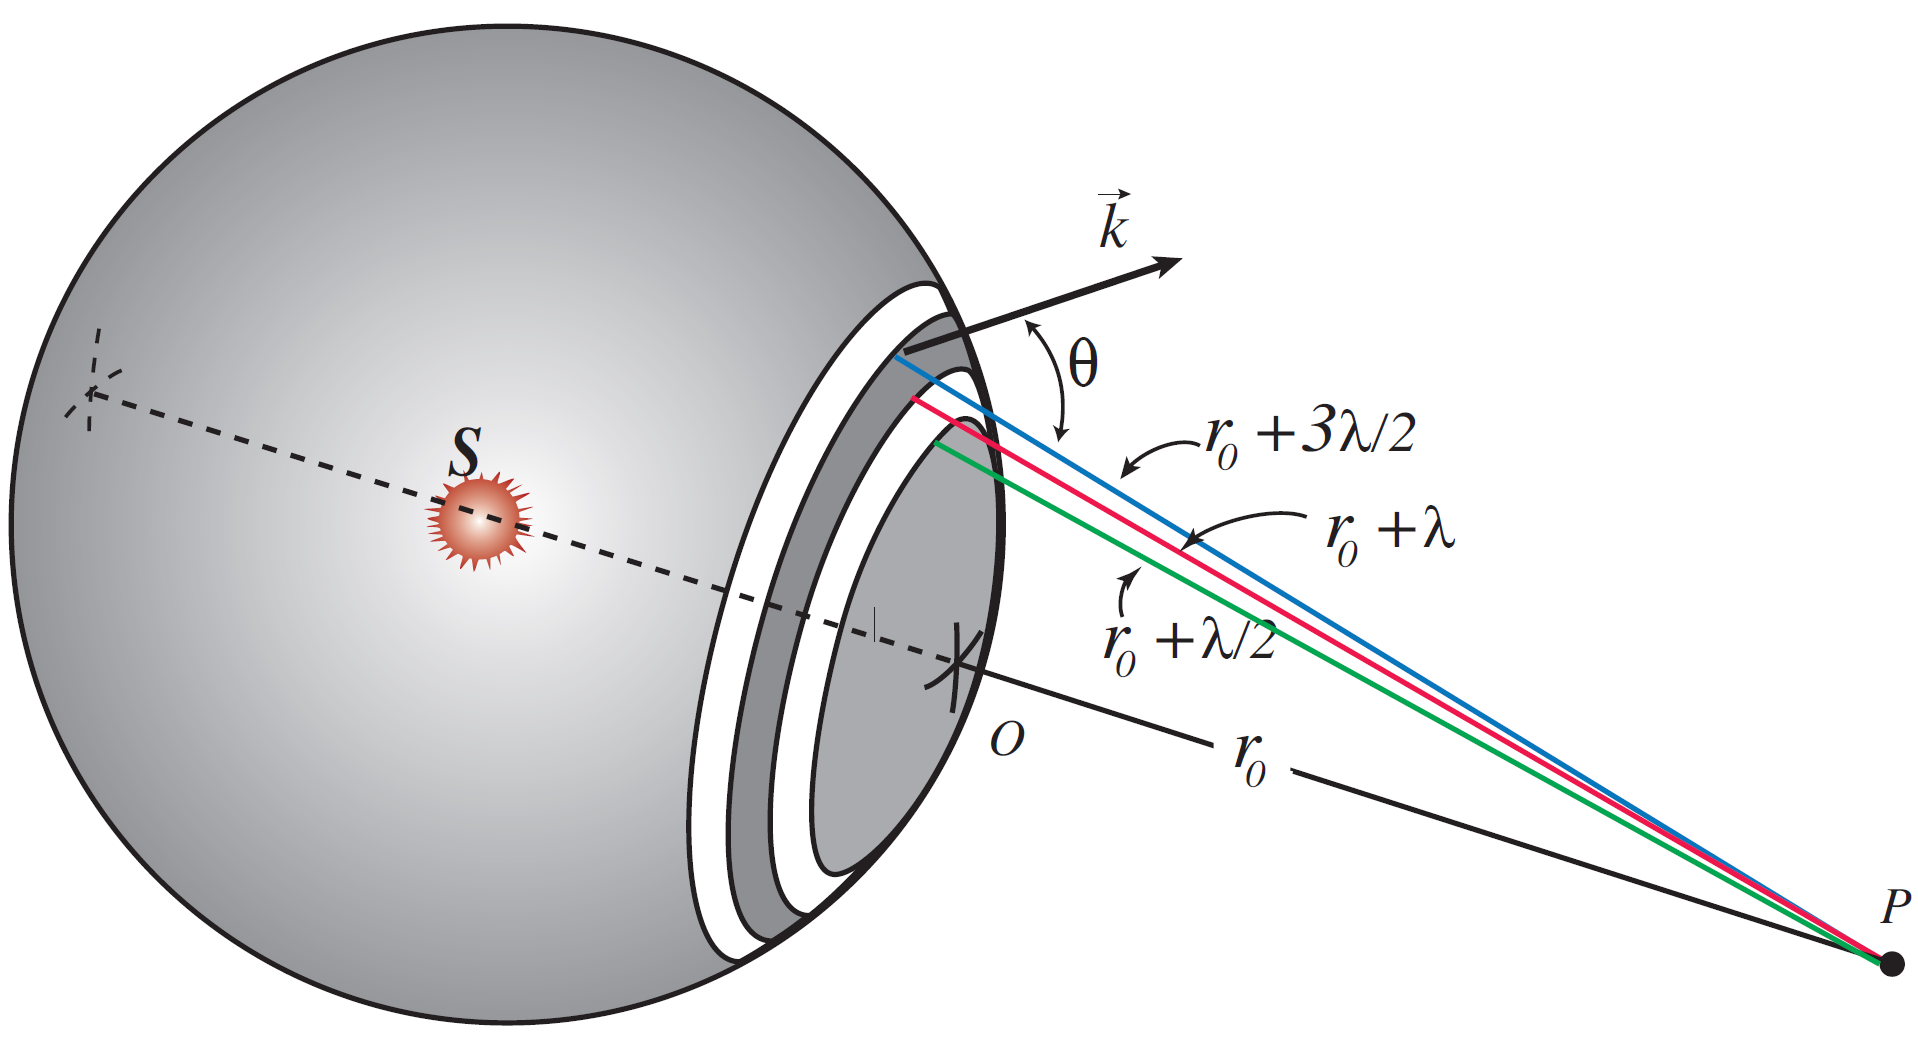
\includegraphics[scale=0.26]{06-Fresnel.png}
    \caption{}
    \label{Fig:06.2-01}
\end{figure}

Existe un método gráfico para analizar cualitativamente varios problemas de difracción que aparecen, principalmente, en configuraciones circulares simétricas. Imaginemos que solo llega a $P$ la primera zona de Fresnel y la dividimos en $N$ subzonas por intersección de esferas centradas en $P$ de radios $r_0+n\lambda /2N$ con $n=1,2 \ldots ,N$. Cada subzona contribuye a la perturbación en $P$, cuya resultante es precisamente la amplitud $E_1$. Como la diferencia de fase en la zona completa, desde $O$ a su borde, es de $\pi$ radiantes (correspondientes a $\lambda /2$), cada subzona se desplaza $\pi /N$ radianes. En la figura $a$  se muestra la suma vectorial $\En_1$ de los fasores de la subzona donde, por conveniencia, se ha tomado $N=10$. \\

\begin{figure}[h!]
    \centering
    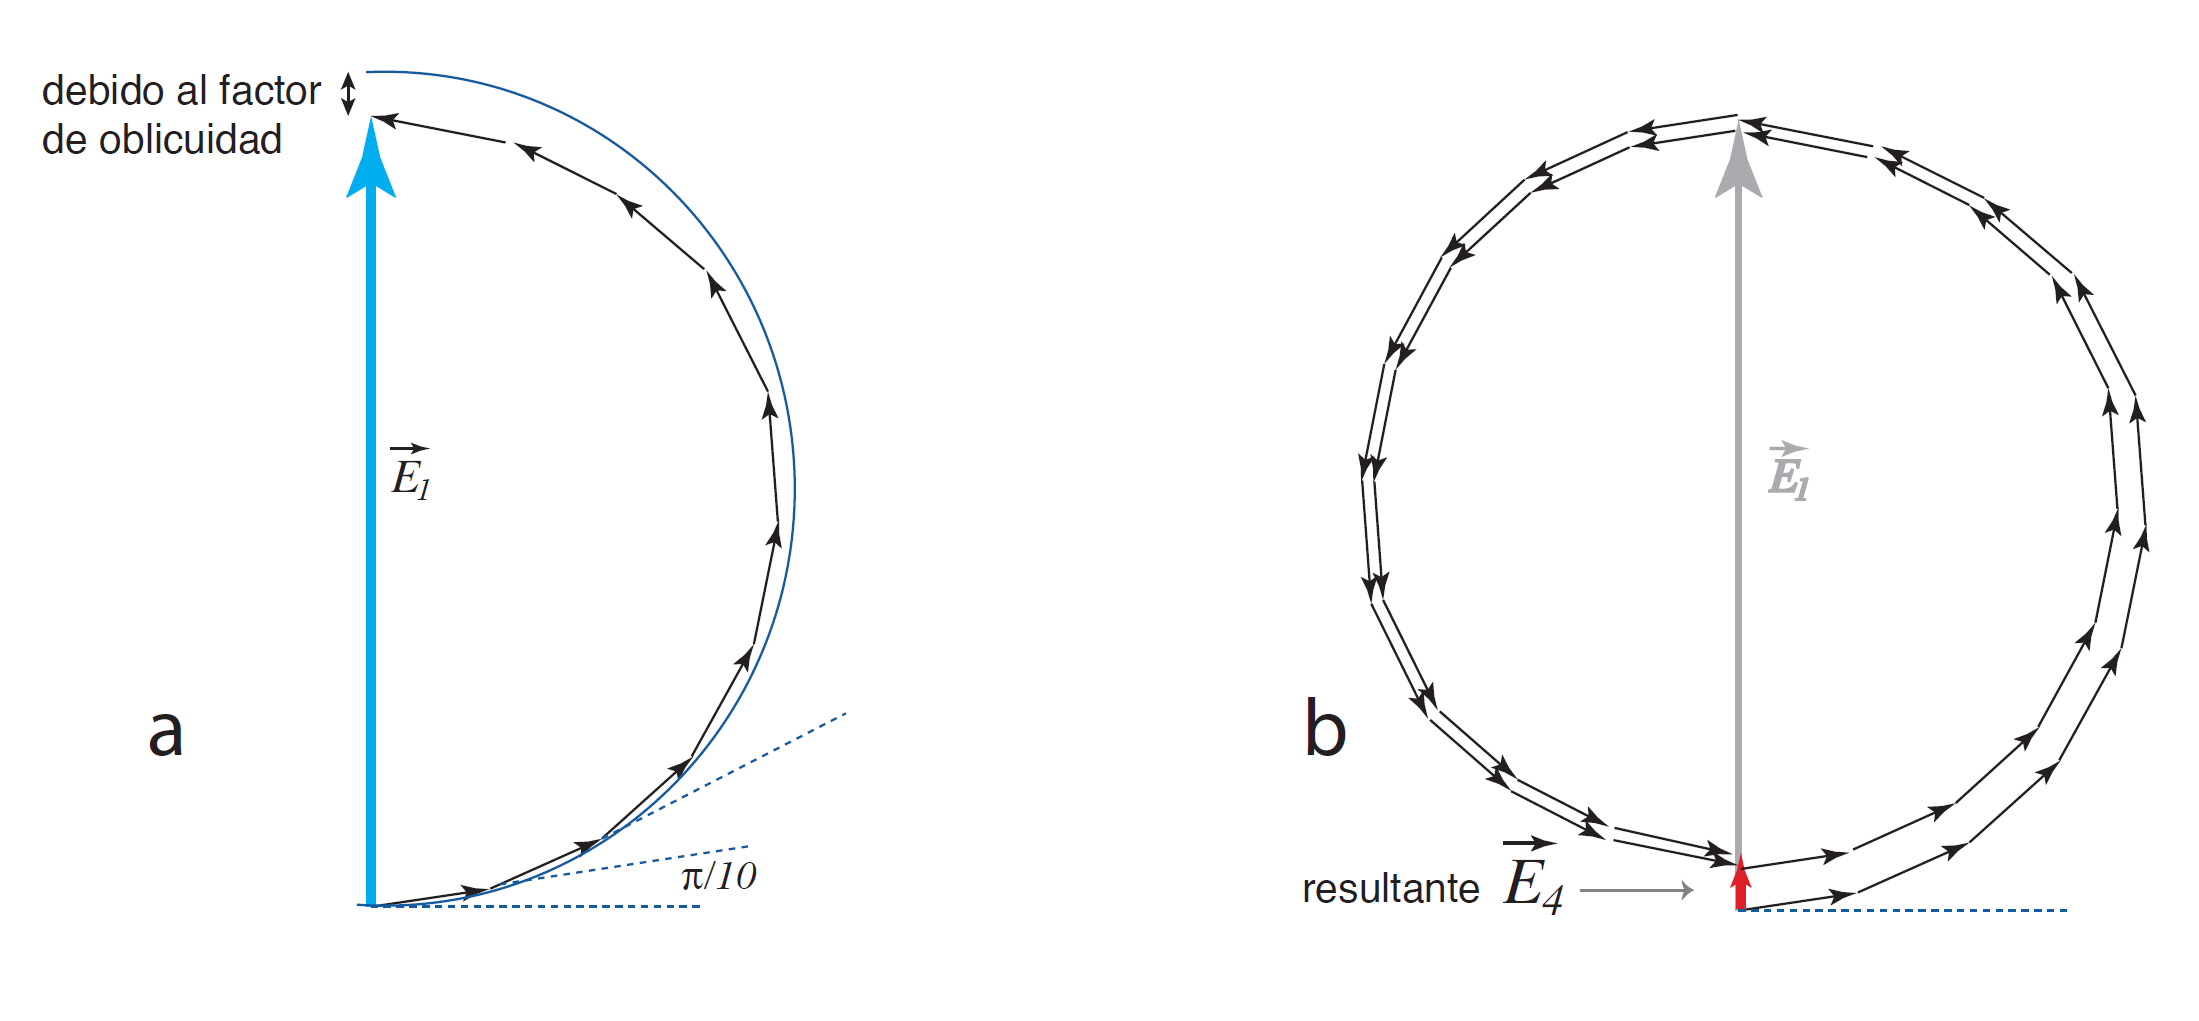
\includegraphics[scale=0.27]{06-Grafico.png}
    \caption{}
    \label{Fig:06.2-02}
\end{figure}

La cadena de fasores se desvía muy ligeramente del círculo, porque al avanzar en la esfera las superficies se van inclinado y disminuyendo ligeramente ya hay que computar los factaores de oblicuidad. Esos factores reducen el peso de zonas que emiten ondas con una dirección privilegiada $\kn$ que forman un ángulo $\theta$ cada vez mayor con $\rn$. Si se van sumando las amplitudes correspondientes a estas 10 subzonas, se va formando una espiral, que se denomina \textbf{curva de vibración}. En la figura $b)$ de \ref{Fig:06.2-02} vemos que se puede contabilizar 4 zonas, $\En_4$, obteniéndose por tanto un valor pequeño de intensidad, lo que ocurre siempre que computemos un número par de zonas, que van neutralizándose una con la anterior, dado que hay un desfase total de $\pi$ radiantes entre zonas consecutivas. \\

En el límite en el que contabilizamos infinitas zonas (es decir que dejamos pasar toda las zonas de Fresnel posible, como si no hubiera obstáculo) la espiral tiende a $1/2$ de la amplitud de la primera zona. Dicho de otra forma, la amplitud que observamos en el punto $P$ si dejamos pasar solo la primera zona es el doble de la que observaríamos si dejáramos pasar toda la onda. Traduciendo a intensidades, tendríamos cuatro veces más intensidad que si dejamos pasar solo la primera zona.  \\

Los resultados de las zonas semiperiódicos de Fresnel y la curva de vibración permiten comprender el comportamiento difractivo de las aberturas circulares, y no solo producida por aberturas circulares. Analicemos el siguiente caso:


\begin{figure}[h!]
    \centering
    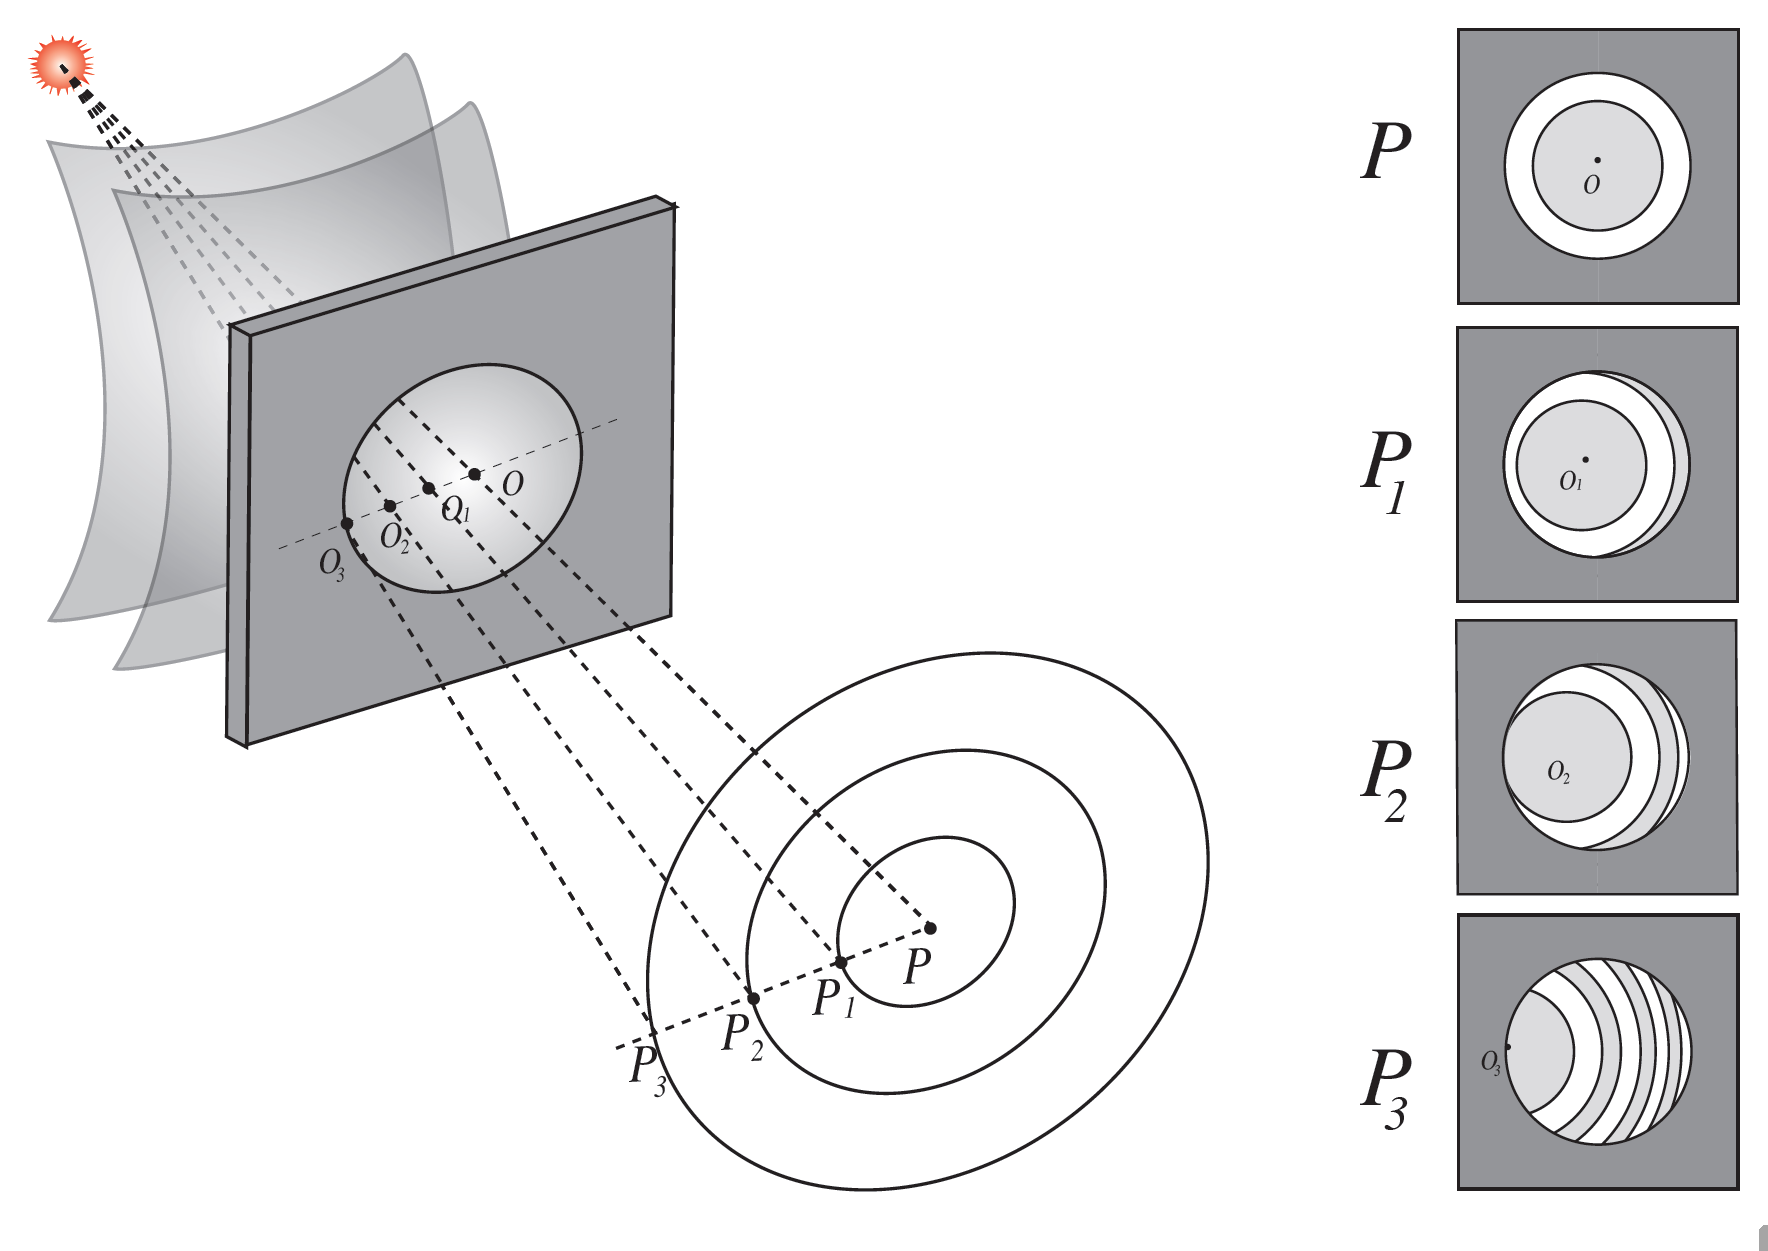
\includegraphics[scale=0.28]{06-Semiperiodicas.png}
    \label{Fig:06.2-03}
    \caption{}
\end{figure}

Supongamos que tenemos una onda esférica que incide sobre una abertura circular. Supongamos que no situamos en un punto $P$ y desde el, a través de la abertura vemos solo las 2 primeras zonas de Fresnel completas (imagen $P$). Como se ha explicado ya, con dos zonas semiperiódicas la intensidad es nula (o casi nula). Supongamos que nos desplazamos ahora transversalmente a un punto $P_1$ desde donde vemos la abertura de forma oblicua (segunda imagen $P_1$). Desde este punto vemos menos la segunda zona (con lo cual ganamos luz en fase con la primera zona). Concluimos pues que tenemos más intensidad. De esta forma podemos ir desplazándonos transversalmente a puntos $P_2,P_3$... viendo diferentes secciones de las franjas, con lo cual obtendríamos máximos y mínimos. Tenemos pues oscilaciones de amplitud (por tanto también de intensidad) al desplazarlo transversalmente. Por simetría ciruclar, esto pasará la desplazarse transversalmente en cualquier dirección. 



\section{Elementos ópticos difractivos}

Una de las consecuencias más interesantes del procedimiento de subdivisión de un frente de onda en \textit{zonas semiperiódicas} propuesto por Fresnel es la posibilidad de modular la intensidad difractada en eje mediante de un tipo de abertura modificada que permita bloquear ciertas zonas semiperiódicas (las que están en oposición de fase), y dejando de trasmitir a las que estén en fase $2\pi$. Este tipo de elemento selectivo de zonas semiperiódicas se conoce como \textbf{Placas zonales de Fresnel}. Consideremos esta posibilidad con detalle, para ello se ilumina con una onda plana las zonas $N$ semiperiódicas de Fresnel ($a_1,a_2,a_3,...,a_N$) y analizando la interferencia de la luz proveniente de estas zonas: 

\begin{equation}
    \psi (0,0,z) = - e^{ik_0z} \parentesis{\left. e^{\frac{ik_0}{2z}\rho^2} \right]_{0}^{a_1} + \left. e^{\frac{ik_0}{2z}\rho^2} \right]_{a_1}^{a_2} +
    \left. e^{\frac{ik_0}{2z}\rho^2} \right]_{a_2}^{a_3} + \cdots + \left. e^{\frac{ik_0}{2z}\rho^2} \right]_{a_{N-1}}^{a_N}  }
\end{equation}

Por razones prácticas vamos a considerar que solo dejamos pasar tres zonas de radios consecutivos que cumplan esta relación:

\begin{equation}
    a_1^2 = b^2 \quad \quad a_2^2=2b^2 \quad \quad a_3^2 = 3b^2 = a^2
\end{equation}
La amplitud será:

\begin{equation}
    \psi (0,0,z) \approx e^{-ik_0z} \parentesis{\ccorchetes{e^{\frac{i2\pi}{\lambda_0}\frac{\lambda_0 D}{2D}}-1} + \ccorchetes{e^{\frac{i2\pi}{\lambda_0}\frac{2\lambda_0 D}{2D}}-e^{\frac{i2\pi}{\lambda_0}\frac{2\lambda_0 D}{2D}}} + \ccorchetes{e^{\frac{i2\pi}{\lambda_0}\frac{3\lambda_0 D}{2D}}-e^{\frac{i2\pi}{\lambda_0}\frac{2\lambda_0 D}{2D}}}}
\end{equation}
De esta forma tenemos que

\begin{equation}
    \psi_j (0,0,D) = - e^{ik_0D} 2 (-1)^j \quad \rightarrow \quad \psi (0,0,D) = e^{-ik_0D}(-2+2-2)=2e^{ik_0D}
\end{equation}

\subsection{Placas zonales de Fresnel}

Una \textbf{placa zonal de Fresnel de amplitud} es un dispositivo que tiene transparentes y opacas alternas, de forma que permite bloquear las regiones semiperiódicas de Fresnel que contribuyen con fase opuesta. De esta forma conseguimos incrementar mucho la intensidad, de tal modo que se produce una redistribución de la energía. Partiendo de un número impar $N$ de zonas, obstruyendo las pares (signo +) o las impares (signo -), obtenemos:

\begin{equation}
    \psi (0,0,D) = \pm \frac{N\pm1}{2} 2e^{ik_0 D} \quad \Rightarrow \quad I(0,0,D) = (N\pm1)^2
\end{equation}

Si en vez de obstruir las zonas semiperiódicas que contribuyen fase opuesta, lo que hacemos es introducirles un desfase $\pi$ adicional, conseguimos que aporten positivamente a la intensidad total. Las placas de Fresnel que logran esto se denominan \textbf{placas zonales de fase}. De este modo partiendo de un número impar $N$ de zonas, y cambiando de fase $\pi$ las pares, tendríamos que:

\begin{equation}
    \psi (0,0,D) = 2N e^{ik_0D}  \ \Rightarrow \ I(0,0,D) = 4N^2
\end{equation}
Vemos que las placas zonales de fase son mas eficientes si $N\gg 1 \Rightarrow 4N^2 \gg (N+1)>N^2 > (N-1)^2$. Por ejemplo para $N=10$ tenemos que $I=400I_0$. 

\subsection{Propiedades ópticas de la placa zonal de fase}

\subsubsection{Foco primario}

El radio de la zona semiperiódica de Fresnel determinada por el contador $m$, viene determinado por el incremento de $m$ semilongitudes de onda respecto al camino óptico seguido por la onda qeu se propagada en eje. Ambas deben confluir en oposición de fase ($m$ impar) o en fase ($m$ par) en el punto $P$ situado la distancia $f_0$. La relación entre el radio de la zona y la posición del máximo (o mínimo) de intensidad en eje se pueden establecer a partir de las relaciones geométricas de la figura:

\begin{equation}
    f_0^2 + a_m^2 = \ccorchetes{f_0 + m \frac{\lambda_0}{2}}^2 \quad \rightarrow \quad f_0^2 +a_m^2 = f_0^2 + 2 f_0 m \frac{\lambda_0}{2}+ \ccorchetes{m \frac{\lambda_0}{2}}^2
\end{equation}
despreciando el último término tenemos que:

\begin{equation}
    a_m = \sqrt{m f_0 \lambda_0}
\end{equation}

\begin{figure}[h!]
    \centering
    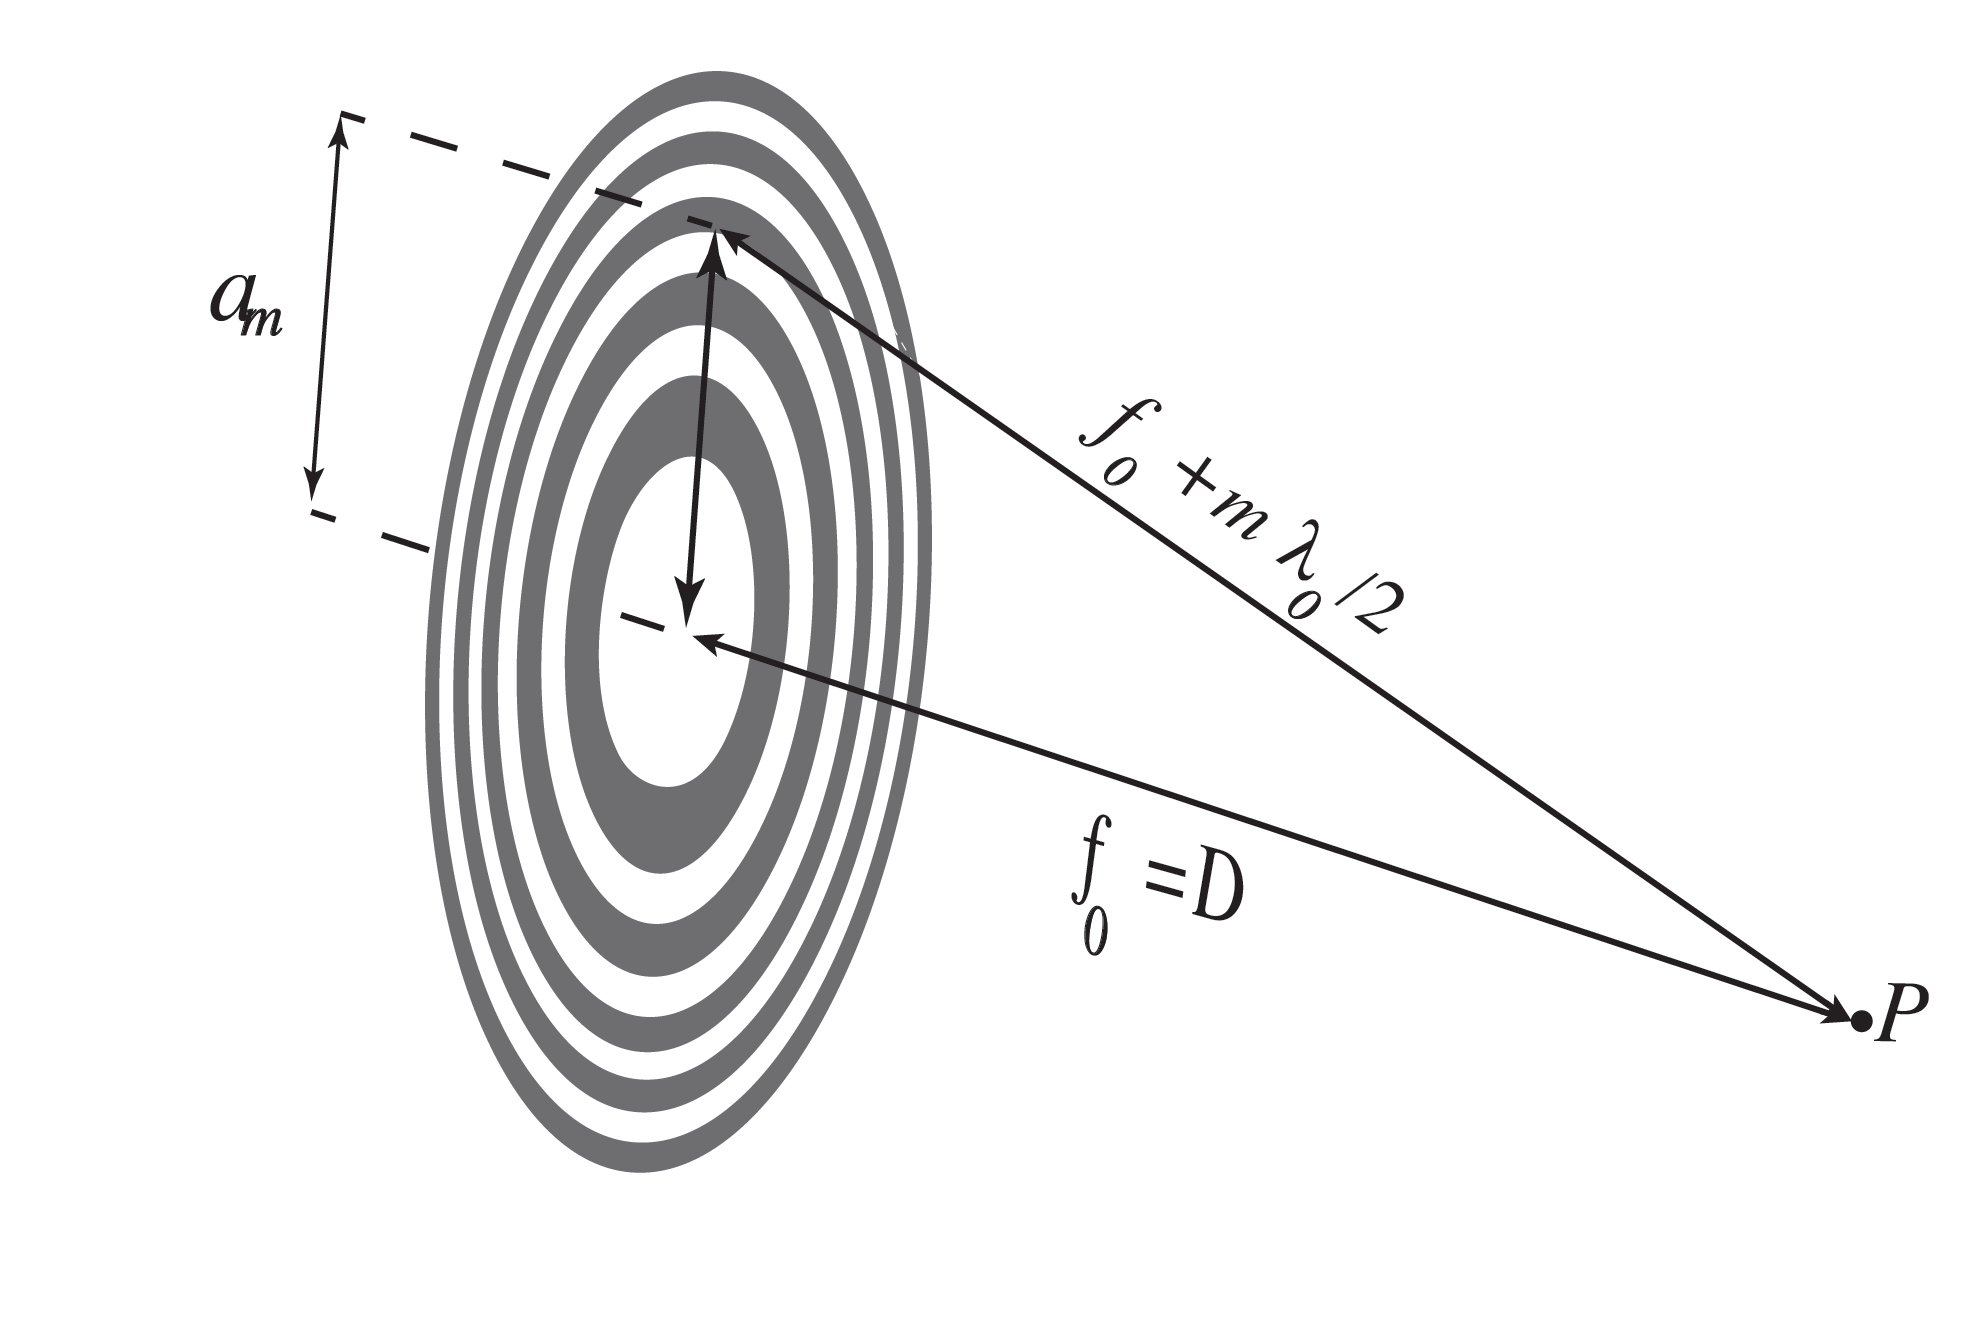
\includegraphics[scale=0.25]{06-Focoprimario.png}
    \caption{}
    \label{Fig:06.3-01}
\end{figure}

\subsubsection{Foco secundario}

\begin{figure}[h!]
    \centering
    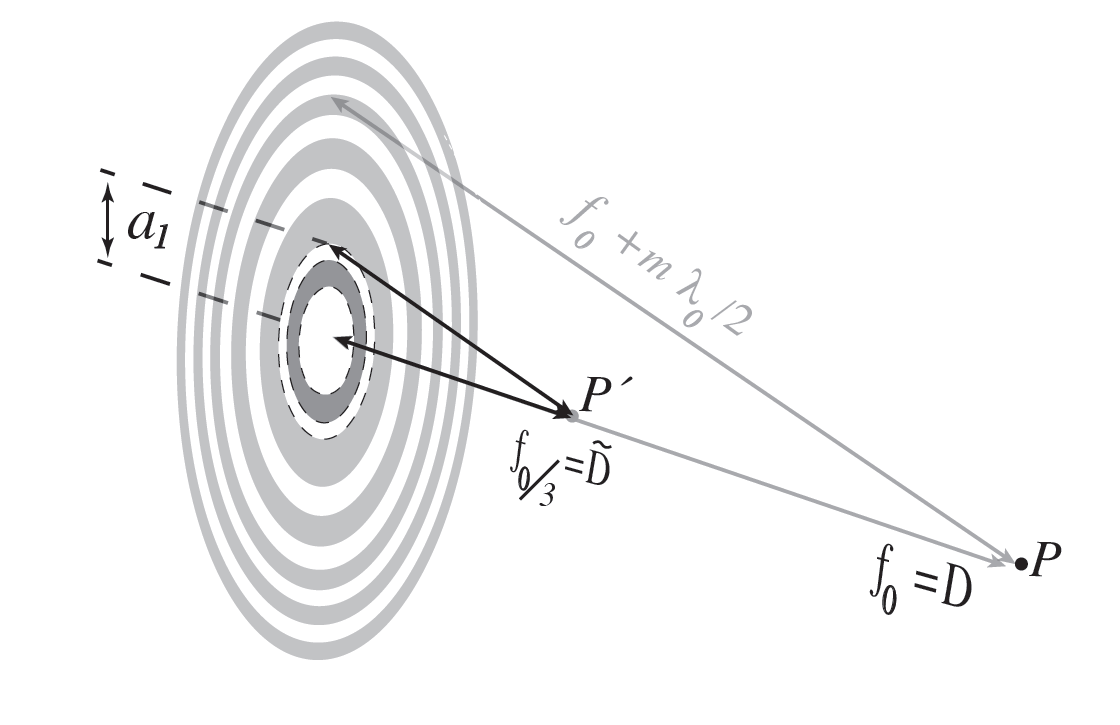
\includegraphics[scale=0.4]{06-Focosecundario.png}
    \caption{}
    \label{Fig:06.03-02}
\end{figure}

Si a su vez, subdividimos la primera zona en tres (o en un número impar de ellas), y repetimos el procedimiento, podremos determinar la intensidad que llega un punto del eje situado ahora a una distancia $\tilde{D}$. El radio de esta primera subzona sería:

\begin{equation}
    \tilde{a}_1^2 = \lambda_0 D = \frac{a_1^3}{3} =  \frac{\lambda_0D}{3}
\end{equation}
generándose también ondas divergentes qeu parecen provenir de focos negativos (virtuales): 

\begin{equation}
    \frac{1}{z_2} - \frac{1}{z_1} = \frac{1}{f_s} = \frac{2s+1}{f_0} = \frac{2s+1}{D} = \frac{(2s+1)\lambda_0}{a_1^2}
\end{equation}


Una \textbf{red de difracción} es un dispositivo compuesto por un agrupamiento de aberturas difractoras, habitualmente de decenas o cientos de aberturas por milímetro. Las placas zonales de Fresnel son un tipo especial de redes de difracción, de periodicidad espacial cuadrática, a diferencia de las redes de difracción de periodicidad lineal. Esta diferencia sustancial implica que para hacer converger a un plano de observación la luz difractada por una red de difracción lineal, se requiere del uso de una lente convergente, tal y como se puede ver en la imagen \ref{Fig:06.3-3}.

\begin{figure}[h!]
    \centering
    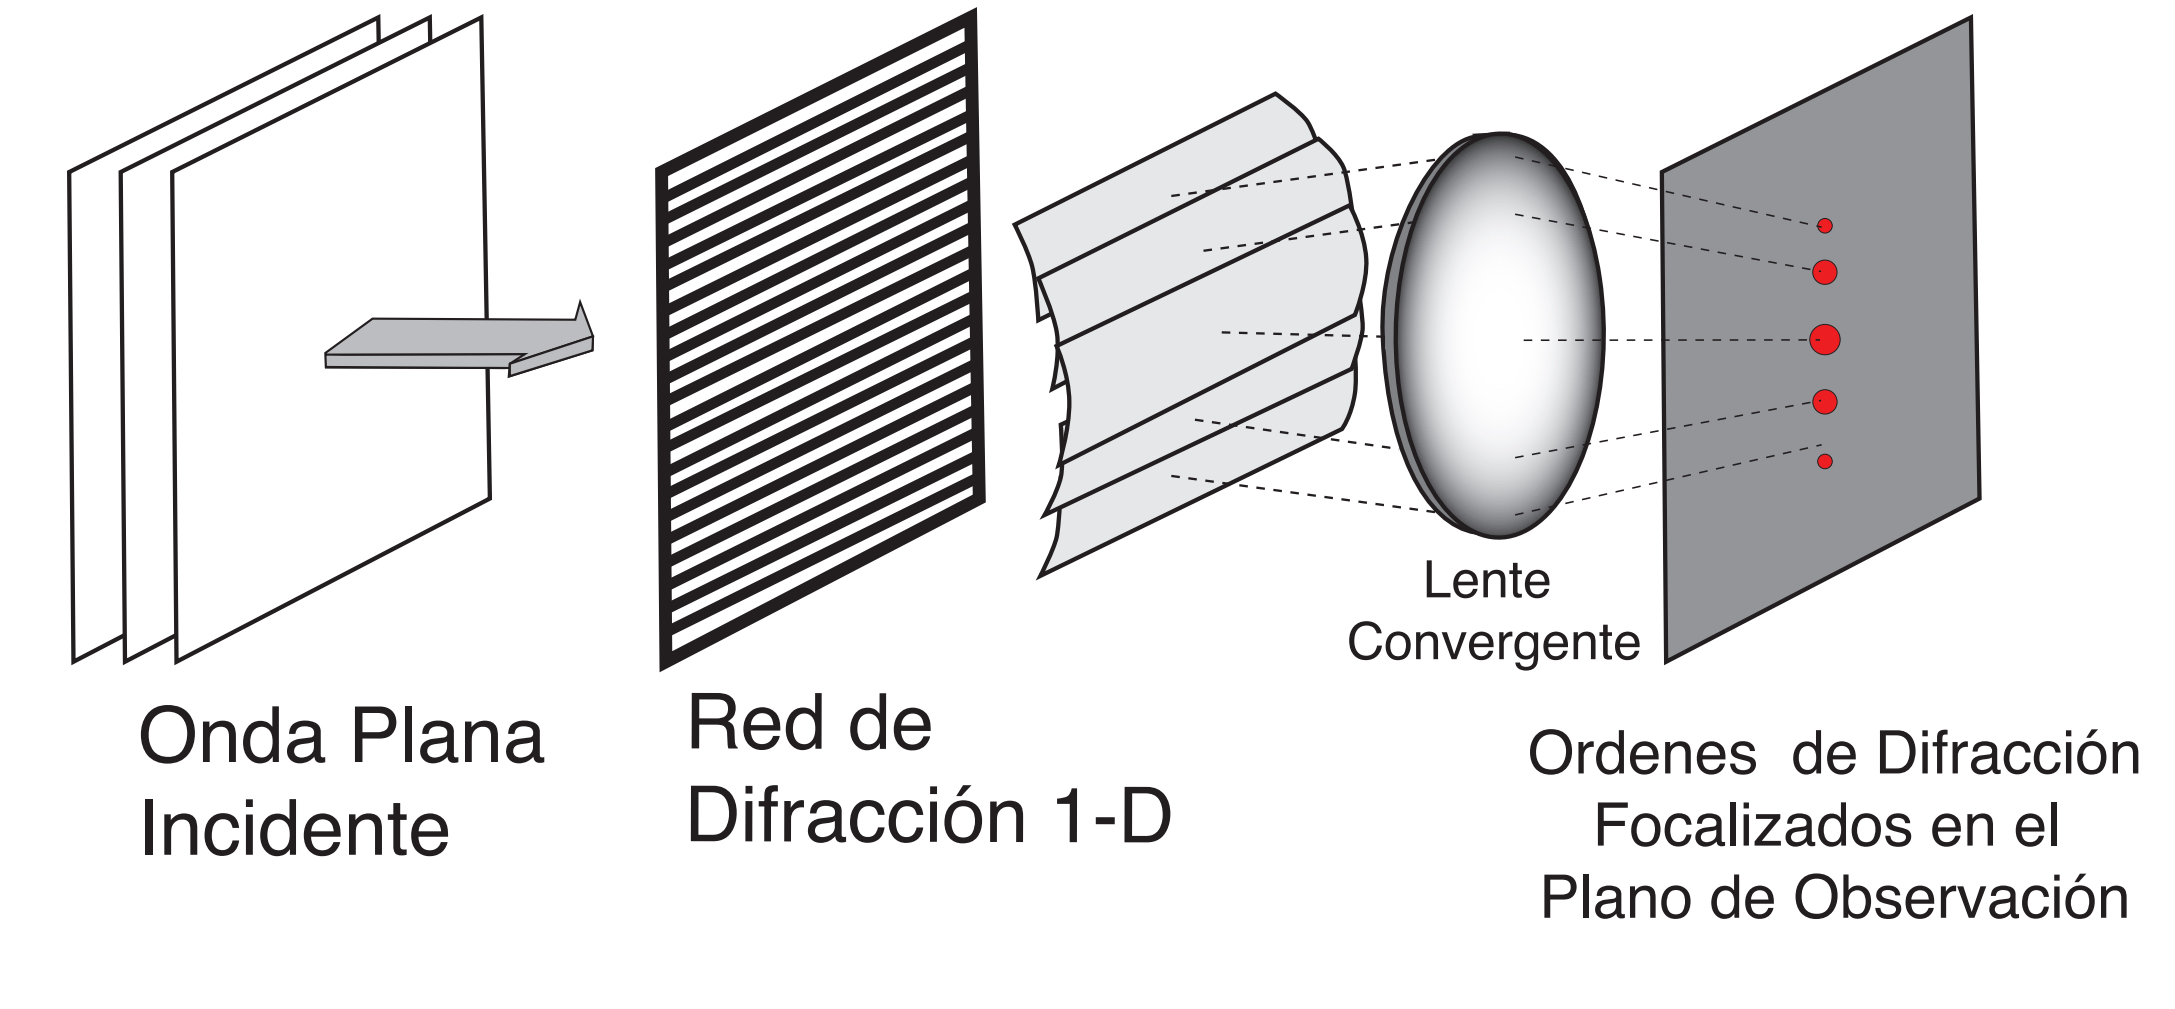
\includegraphics[scale=0.2]{06-Placazonal.png}
    \caption{}
    \label{Fig:06.3-03}
\end{figure}

Sin emgargo en una placa zonal de fase con periodicidad cuadrática, la convergencia va implícita en este factor y por tanto no requiere el uso de un elemento de fase cuadrática como es la lente convergente. 

\begin{figure}[h!]
    \centering
    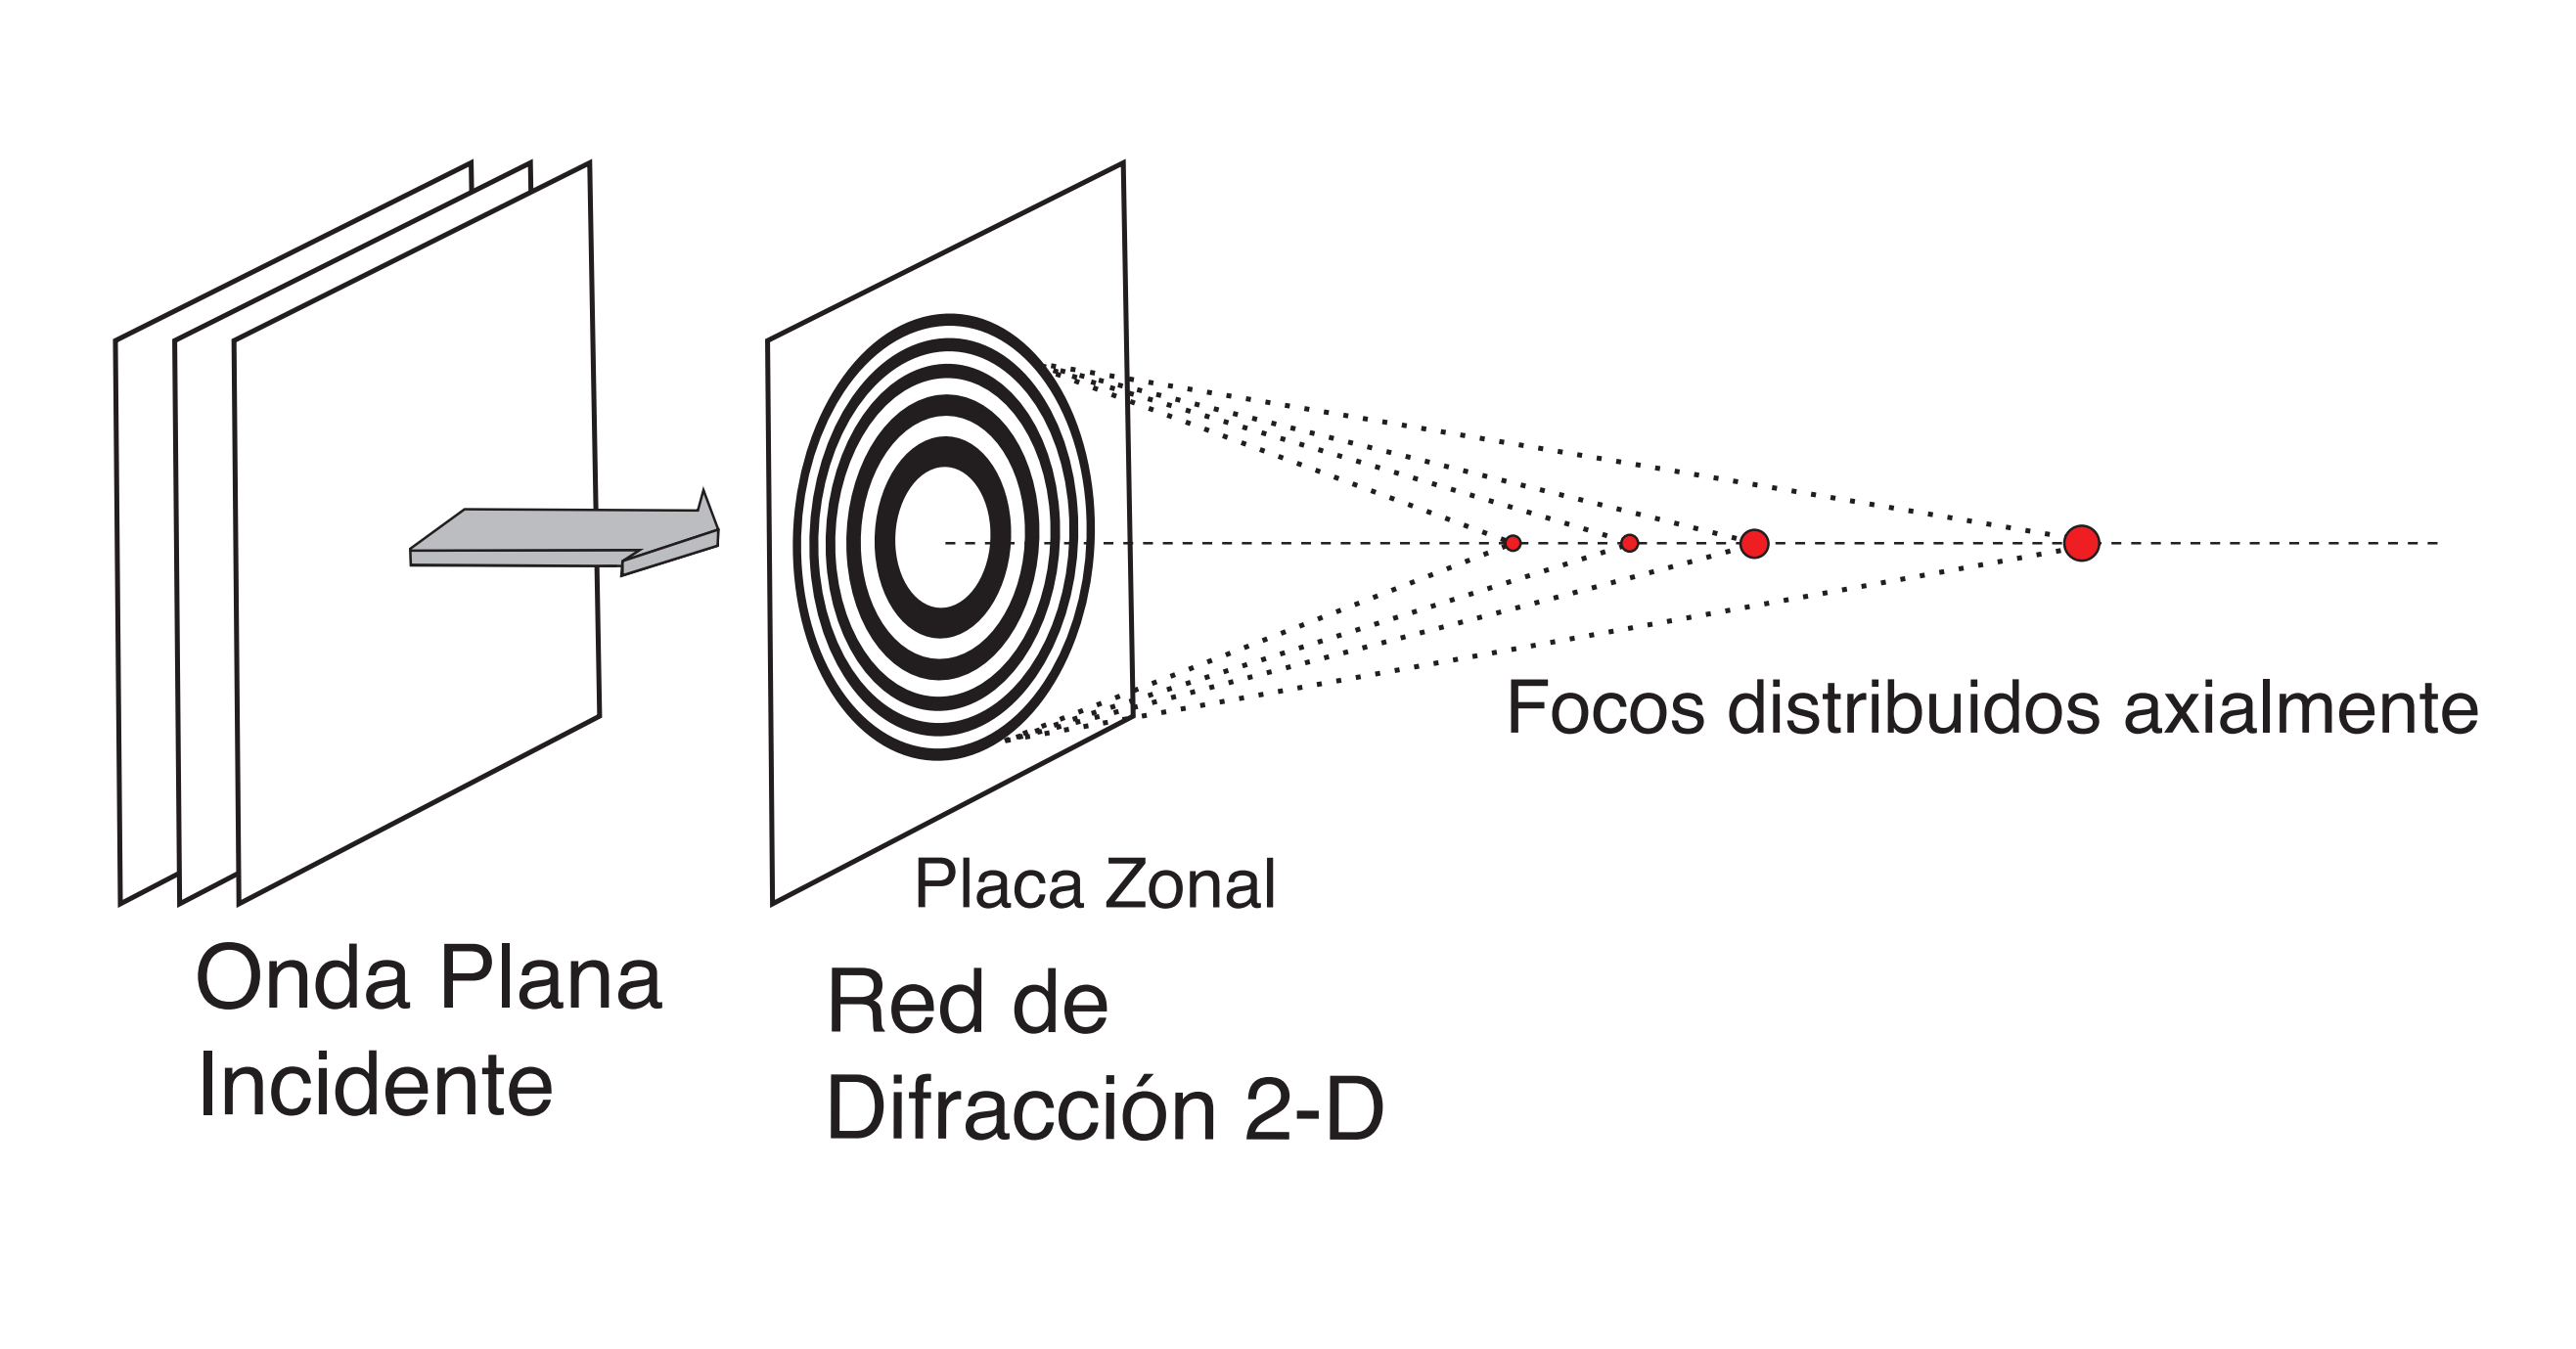
\includegraphics[scale=0.15]{06-Placazonal2D.png}
    \caption{}
    \label{Fig:06.3-04}
\end{figure}


\subsection{Tipos de placa zonales}

\subsubsection{Placa zonal de fresnel: amplitud}

Partiendo de una función de trasmisión que define una placa zona lde Fresnel de la siguiente forma:

\begin{equation}
    t_{FZP} (r) = \left\lbrace \begin{array}{ll}
       1  &  \ r_{2m}^2 \leq r^2 < r_{2m+1}^2 \\
       0  &  \ r_{2m+1}^2 \leq r^2 < r_{2m+2}^2 \\
    \end{array} \right.
\end{equation}
Haciendo un desarrollo en serie de esta función de trasmisión tenemos que:

\begin{equation}
    t_{FZP} = \frac{1}{2} + \sum_{j = - \infty}^{\infty} \frac{1}{i \pi j} \exp \ccorchetes{i \frac{\pi j}{\lambda f} r^2} \tquad  j \in \text{impar}
\end{equation}
Es inmediato comprobar que los términos del sumatorio corresponden a las ondas esféricas divergentes (si $j>0$) o convergentes (si $j<0$) de los focos dados por la expresión:

\begin{equation}
    f_j = - \frac{f}{j} = - \frac{r_1^2}{j \lambda}, \ j \text{impar} \ \Rightarrow \ \pm f,\pm f/3,\pm f/5, \pm f/7, \ldots
\end{equation}
La eficiencia (intensidad de cada onda en relación a la intensidad incidente) es:

\begin{equation}
    n_{\pm j} = \left| \frac{1}{i\pi j} \right|  \ j \ \text{impar}
\end{equation}
por lo que $\eta_{\pm 1} \approx 10\%$.


\subsubsection{Placa zonal de fresnel: fase}

Si partimos de una función de trasmisión de fase, que define una placa zonal de Fresnel de la siguiente manera:

\begin{equation}
    t_{FZP} (r) = \left\lbrace \begin{array}{ll}
       1  &  \ r_{2m}^2 \leq r^2 < r_{2m+1}^2 \\
       -1  &  \ r_{2m+1}^2 \leq r^2 < r_{2m+2}^2 \\
    \end{array} \right.
\end{equation}
Haciendo el desarrollo en serie de esta función 

\begin{equation}
    t_{FZP} =  \sum_{j = - \infty}^{\infty} \frac{2}{i \pi j} \exp \ccorchetes{i \frac{\pi j}{\lambda f} r^2} \tquad  j \in \text{impar}
\end{equation}
Nuevamente podemos comprobar que los términos del sumatorio corresponden a las ondas esféricas divergentes (si $j>0$) o convergentes (si $j<0$) de los focos dados por la expresión:

\begin{equation}
    f_j = - \frac{f}{j} = - \frac{r_1^2}{j \lambda}, \ j \text{impar} \ \Rightarrow \ \pm f,\pm f/3,\pm f/5, \pm f/7, \ldots
\end{equation}
Aun teniendo el mismo número de focos que la placa zonal de fase de amplitud, la eficiencia en los ordenes +1 y -1 es mayor:

\begin{equation}
    \eta_{\pm j} = \left|\frac{2}{i\pi j}\right|^2 \ j \text{impar}
\end{equation}
tal que $\eta_{\pm1}\approx 40\%$.

\subsubsection{Placa zonal de Gabor}

En este caso tenemos una función de trasmisión de la forma:

\begin{equation}
    t_{SPZ} (r) = \frac{1}{2} \ccorchetes{1+\beta \sin \parentesis{\frac{\pi}{\lambda f} r^2}} \quad \beta \leq 1
\end{equation}
o usando la fórmula de Euler:
\begin{equation}
    t_{SPZ} (r) = \frac{1}{2} + \frac{\beta}{4i} e^{i\frac{\pi j}{\lambda f} r^2} -
    \frac{\beta}{4i} e^{i\frac{\pi j}{\lambda f} r^2}
    \quad \beta \leq 1
\end{equation}
En esta ocasión solo se obtienen tres ondas, una onda plana y dos esféricas, una convergente y otra divergente, que se focalizan en $\pm f$, con eficiencia:

\begin{equation}
    \eta_{\pm 1} = \left| \frac{1}{4i} \right| \approx 6.25 \% \quad \beta=\pm 1
\end{equation}
Esta sería la placa zonal más parecida a una lente convencional, pero con focos de peor eficiencia, y por tanto no competitiva para substituir a lentes refractivas. 

\subsubsection{Placa sinusoidal zonal de fresnel}

Podría aumentarse la eficiencia haciendo esta última placa zonal como elemento de fase. Así la función de trasmisión:

\begin{equation}
    t_{SPZ} (r) = \exp \ccorchetes{ \frac{i}{2} \parentesis{\pi+\beta \sin \parentesis{\frac{\pi}{\lambda f} r^2}}}r \quad \beta \leq 1
\end{equation}
desarrollando en serie:
\begin{equation}
    t_{SPZ} (r) = e^{i \frac{\pi}{2}} \sum_{j = - \infty}^{\infty}  J_j \parentesis{\frac{\beta}{2}} \exp\ccorchetes{i j \frac{\pi}{\lambda f} r^2}
\end{equation}
En esta ocasión solo se obtienen tres ondas, una onda plana y dos esféricas, una convergente y otra divergente, que se focalizan en $\pm f$, con eficiencia:

\begin{equation}
    \eta_{\pm 1} = \left| \frac{1}{4i} \right| \approx 6.25 \% \quad \beta=\pm 1
\end{equation}
donde $J_j$ son \textit{funciones de Bessel}. Estas placas se obtienen por blanqueamiento de la anterior. Tenemos pues elementos de fase con múltiples órdenes difractados, que focalizan en:

\begin{equation}
    f_j = - \frac{f}{j} = - \frac{r_1^2}{j \lambda} \ \Rightarrow \ \pm f, \pm f/2, \pm f/3, \ldots
\end{equation}
La eficiencia en este caso viene dada por

\begin{equation}
    \eta_{\pm j} = \left| \exp \left\lbrace i\frac{\pi}{2} \right\rbrace J_j \parentesis{\frac{\beta}{2}}^2 \right| 
\end{equation}
con $\eta_{\pm 1} \approx 34 \%$ con mejores resultados pero infinitos focos.

\subsection{Placa zonal de Kinoform}

Es posible diseñar y construir un tipo de placa zonal que presente un comportamiento similar a una lente. Debe ser una placa zonal con pocos focos y de alta eficiencia.  Este tipo de placas se denominan \textbf{placas zonales de Kinoform}. \\

La placa zonal de Kinoform es un elemento de fase qeu introduce un salto de fase $2\pi$ en zonas sucesivas, mediante modulación del relieve (que es un hiperboloide) del elemento. Así se produce un espectro de Fourier asimétrico y mejora la eficiencia de la difracción. Analizando la fase acumulada por la onda al atravesar la zona central (eje óptico), la placa zonal introduce una fase debido a su espesor que, como veremos, en la zona central decrece al alejarse del eje. Al ser mas fina la lámina, introduce menos fase, pero esta se compensa con el hecho de tener que recorrer más camino para llegar al punto focal situado en eje, con lo cual todas las ondas llegan a ese punto, en fase. En las demás zonas ocurre algo similar. \\

El perfil de la placa ya hemos dicho que eran hiperboloides, donde el \textit{espesor} $z(r)$: 

\begin{equation}
    z(r) = \frac{n_p}{n_p^2-n_e^2} \quad \eta=\frac{n_e}{n_p} (n_p-n_e)^2  \quad \delta = \frac{n_e}{n_p} \sqrt{n_p^2 - n_e^2} \quad \lambda_0 = n_e \lambda_e = n_p \lambda_p 
\end{equation}
en aproximación paraxial tenemos un perfíl parabólico:

\begin{equation}
    z(r) = z_{\max} \parentesis{m - \frac{r^2}{2 \lambda_0 f}} \quad z_{\max} = \frac{\lambda_0}{(n_p-n_e)n_e} 
\end{equation}
La función de trasmisión de una placa de Kinoform viene dada por:

\begin{equation}
    t_{K} (x,y) = e^{i\phi(x,y)} \quad \phi(x,y) = \phi (r) = \frac{2\pi}{\lambda_0} (n_p-n_e) z_{\max} \parentesis{m-\frac{r^2}{2 \lambda_0 f}} 
\end{equation}
la función de trasmisión desarrollada en la serie de fourier:

\begin{equation}
    t_{K} (x,y) = \sum_j C_j \exp \ccorchetes{i \frac{2\pi j}{r_1^2}r^2} \quad C_j = e^{i2\pi \alpha m} \ccorchetes{\frac{e^{-i2\pi (\alpha+j)}-1}{2 \pi (\alpha +j)}}  \quad \alpha = (n_p - n_e) \frac{z_{\max}}{\lambda_0}
\end{equation}
La eficiencia de cada orden es de 

\begin{equation}
    \eta_j = |C_j|2 = \sinc^2(\alpha+j)
\end{equation}
El parámetro $\alpha$ se denomina \textbf{parámetro de diseño} ya que puede establecerse de forma que la eficiencia sea máxima en un orden dado y cero en el resto: 

\begin{itemize}
    \item Si $\alpha=1$ solo tendremos el orden +1, obteniendo así una lente difractiva monofocal de alta eficiencia. \\
    \item Si $\alpha=0.5$ los órdenes 0 y 1 tiene una eficiencia del 40\%, puede considerarse una lente bifocal (despreciando órdenes superiores, que se reparten el 20\% de la energía restante). Este tipo de placaz zonales focales sirven para sustituir el cristalino en casos de catarartas. 
\end{itemize}

\chapter{Difracción de Fraunhofer}
\section{Integral de Fraunhofer}

Ya hemos tratado en el capítulo \ref{Sec:5} la aproximación de Fresnel y la aproximación de Fraunhofer. La aproximación de Fresnel es también conocida como la \textit{aproximación parabólica}, y eso ha hecho más asequible la resolución de la integral, pero solo para puntos del eje en aperturas circulares/cuadradas. En otros casos necesitábamos métodos alternativos como el de las zonas semiperiódicas de Fresnel. \\

La resolución de la integral se simplificará notablemente si fuese posible eliminar el factor $x_0^2$ e $y_0^2$. Esto se consigue imponiendo la condición de que este factor sea muy pequeño, esencialmente reduciendo las dimensiones de la abertura frente a la separación axial de los planos (o aumentando $\lambda$). Cuando se cumple esto estamos ante la difracción de Fraunhofer. Ya hemos presentado la integral de Fraunhofer en la ecuación \ref{Ec:05.04-12}, pero dado que va a ser usada de manera constante en este tema la escribimos aquí:

\begin{equation}
     \psi (x,y,z)  \approx \Ecal_0 (x,y,z) \int_A \psi (x_0,y_0,z) e^{-i \frac{2\pi}{\lambda_0 z} \ccorchetes{xx_0+yy_0}} \D x_0 \D y_0
\end{equation}
donde $\Ecal_0(x,y,z) = \frac{-i}{\lambda_0 z} e^{ik_0z} e^{\frac{ik_0}{2z}(x^2+y^2)}$, donde podemos usar las \textbf{frecuencias espaciales} $f_x=x/z\lambda_0$ 
y $f_y=y/z\lambda_0$ para crear así una suerte de trasformada de Fourier, tal que

\begin{equation}
    \psi (x,y,z) = \Ecal_0(x,y,z) \TF [\psi (x_0,y_0)]
\end{equation}
La forma más práctica para que se cumplan las condiciones de la aproximación de Fraunhofer es la utilización de una lente esférica convergente, cuyo factor cuadrático es idéntico (pero con signo negativo>) al factor de fase que se quiere eliminar. 

\section{Estudio canónico}
\subsection{Abertura rectangular}

Sea una abertura rectangular, con una función de trasmisión definida como


\begin{equation}
    t(x_0,y_0) \left\lbrace
    \begin{array}{ll}
        1 \ & |x_0|\leq a, \ |y_0|\leq b  \\
        0 \ & |x_0|> a, \ |y_0|>b
    \end{array}
    \right.
\end{equation}
iluminando normalmente la abertura con una onda plana de amplitud unidad. Dado que el problema integral es separable e introduciendo las coordenadas de la abertura en los límites de integración correspondientes, tenemos que la integral resultante viene dada por

\begin{equation}
    \psi (x,y,z) = \Ecal_0 \int_{-a}^{+a} \int_{-b}^{-a} e^{i2\pi(f_xx_0+f_yy_0)} \D x_0 \D y_0
\end{equation}
de tal modo que podemos obtener:

\begin{equation}
    \psi (x,y,z) = 4 \Ecal_0 \ccorchetes{a \sinc \parentesis{\frac{k_0 a}{z}x}}  \ccorchetes{b \sinc \parentesis{\frac{k_0 b}{z}y}}\label{Ec:07.2-03}
\end{equation}
Por lo que la intensidad máxima viene dada por $I_0 = 4^2 |\Ecal_0|^2 (ab)^2$. La intensidad general viene dada por: 
\begin{equation}
    I (x,y,z) =I_0 \ccorchetes{\sinc^2 \parentesis{\frac{k_0 a}{z}x}}  \ccorchetes{ \sinc^2 \parentesis{\frac{k_0 b}{z}y}} \label{Ec:07.2-04}
\end{equation}
Llamamos \textit{máximo principal} al máximo que hay en el punto $x=y=0$ del plano de observación. Dado que la función obtenida es un senc, lógicamente existirán máximos y mínimos a lo largo de los ejes x e y, obteniendo así los máximos cuando el seno se hace máximo y mínimos cuando se hace mínimo. Así:

\begin{itemize}
    \item \textbf{Mínimos nulos:} obtendremos mínimos en el eje x y en el eje y en aquellos valores que verifiquen

    \begin{equation}
        x_m = m \frac{z\lambda_0}{2a} \tquad y_n = n \frac{z \lambda_0}{2a}
    \end{equation}

    \item  \textbf{Máximos secundarios:} en este caso los máximos secundarios se hallan derivando la función $\sinc(x)$ e igualando a cero, obteniendo una ecuación trascendente:

    \begin{equation}
        \tan \parentesis{k_0 \frac{a}{z}x} = k_0 \frac{a}{z}x \tquad  
        \tan \parentesis{k_0 \frac{b}{z}y} = k_0 \frac{b}{z}y
    \end{equation}
    Las soluciones de esta ecuación se obtiene gráficamente, de tal modo que podemos hallar una solución aproximada:

    \begin{equation}
        k_0 \frac{a}{z} x_m \approx \parentesis{m\pm \frac{1}{2}} \tquad 
        k_0 \frac{b}{z} y_n \approx \parentesis{n \pm \frac{1}{2}}
    \end{equation}
\end{itemize}

Así obtenemos valores de la intensidad en la difracción de Fraunhofer de una abertura rectangular de dimensiones $2a \times 2b$ es:

\begin{equation}
    I_{mn} \approx \frac{I_0}{(m\pm1/2)^2(n\pm1/2)2 \pi^4}
\end{equation}

\begin{figure}[h!]
    \centering
    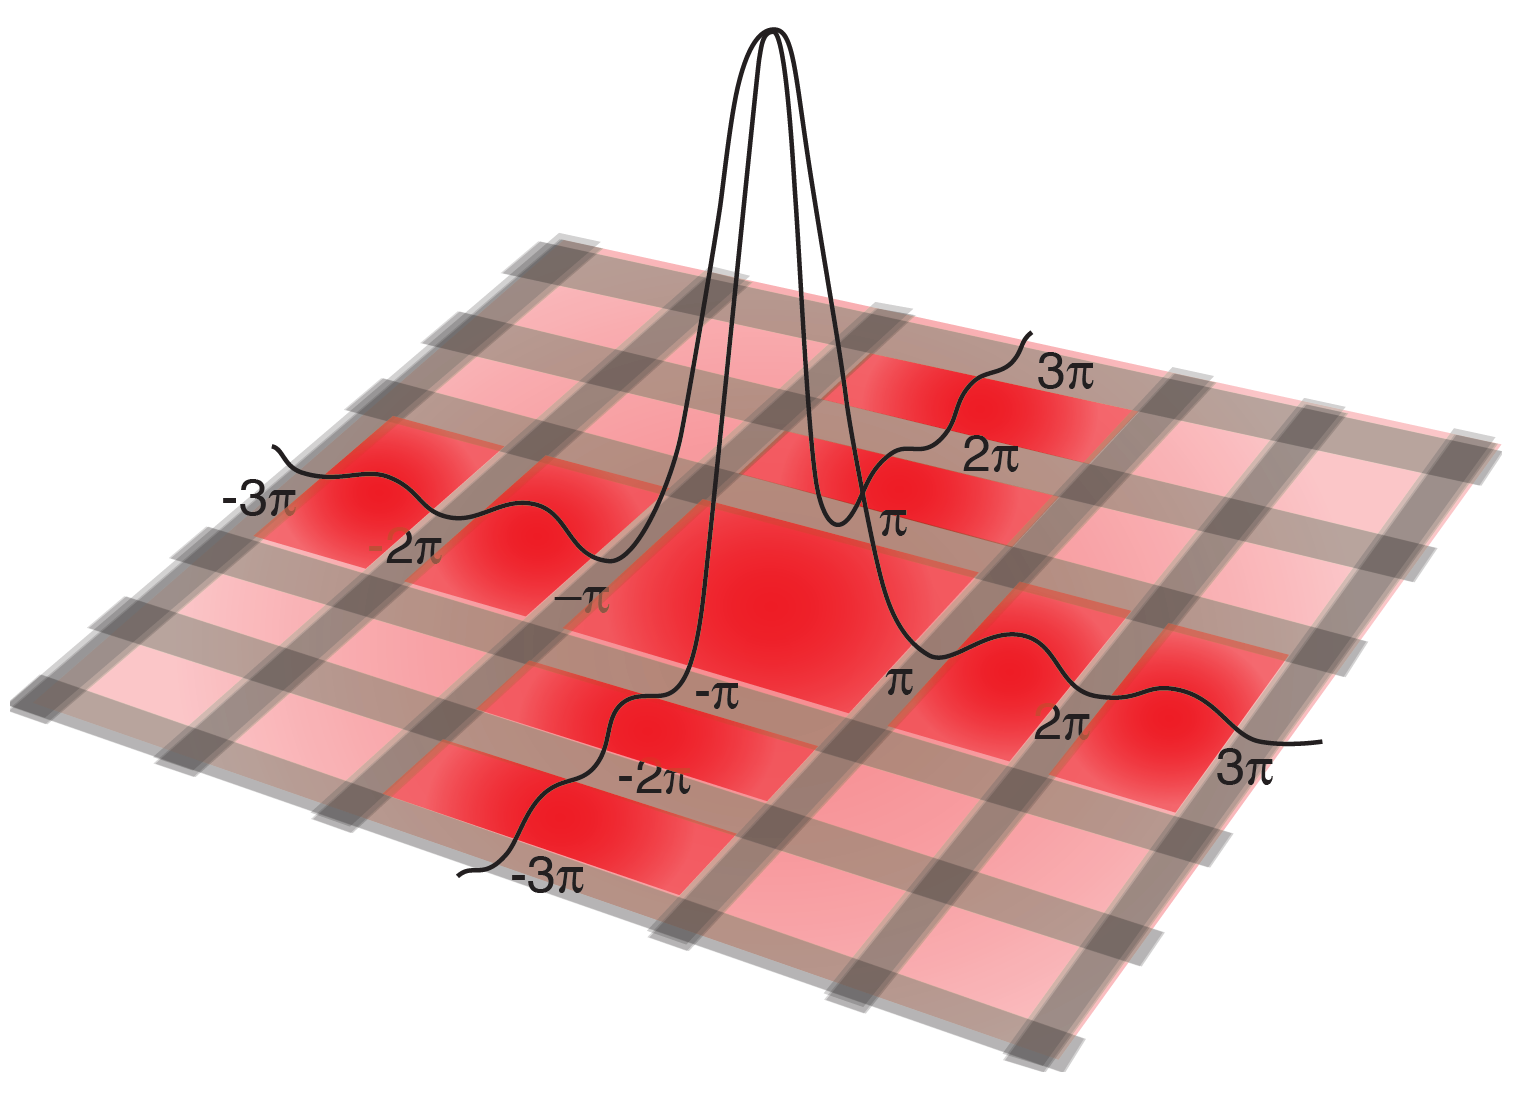
\includegraphics[scale=0.35]{07-Extremos.png}
    \caption{}
    \label{Fig:07.2-01}
\end{figure}


\subsection{Abertura lineal}

Analizando la expresión \ref{Ec:07.2-03}, si consideramos que una de las dimensiones de la abertura, por ejemplo la altura $b$, va aumentando, entonces $I_y(f)$ va colapsando a lo largo de $y$ y por tanto $I_y(f)$ va tendiendo a cero, excepto en las proximidades del eje $y$. Cuando $y=0$ da igual lo grande que sea $b$, seguiremos teniendo un máximo de dicho $\sinc$. Por otro lado la intensidad en $I_x(f)$ permanece invariable, en virtud de la inseparabilidad de la  e Fraunhofer. De este modo tenemos que la intensidad de una rendija que verifica que $a\ll b$ seguirá la ecuación de amplitud

\begin{equation}
    \psi_{\mathrm{rendija}} =  \Ecal \ccorchetes{2a \frac{\sin (k_0 a z /z)}{k_0ax/z}} \delta (y)
\end{equation}
siendo la intensidad

\begin{equation}
    I_{\mathrm{rendija}}(x,y,z) = I_0 \sinc^2 \parentesis{k_0 \frac{a}{z}x} \tquad I_0 = |\Ecal|^2 4a^2
\end{equation}


\subsection{Abertura circular}

Partiendo de la integral de difracción-Fraunhofer para las coordenadas polares, tenemos que

\begin{equation}
    \psi (\rho,f) = \Ecal_0 (\rho,f) \int_0^a \int_0^{2\pi} e^{i\frac{k_0}{f} \rho \rho_0 \cos (\phi-\phi_0)} \rho_0 \D \rho_0 \D \phi_0
\end{equation}
A esta clase de integrales las llamamos las \textbf{funciones de Bessel}, de tal modo que 

\begin{equation}
    \psi (\rho,f) = \Ecal_0 \frac{2 \pi a f}{k_0 \rho} J_1 \parentesis{\frac{k_0 \rho a}{f}}
\end{equation}

\section{Instrumento óptico}
\subsection{Teoría de Airy}

La función de Bessel tiene un comportamiento similar al de un seno, de tal forma que la función de Airy tiene un comportamiento similar a un $\sinc$. Los máximos y mínimos de la fitura de Airy deben calcularse numéricamente. El resultado más relevante de los efectos ópticos es la anchura radial o máximo central (principal) de la figura de Airy. 

\begin{figure}[h!]
    \centering
    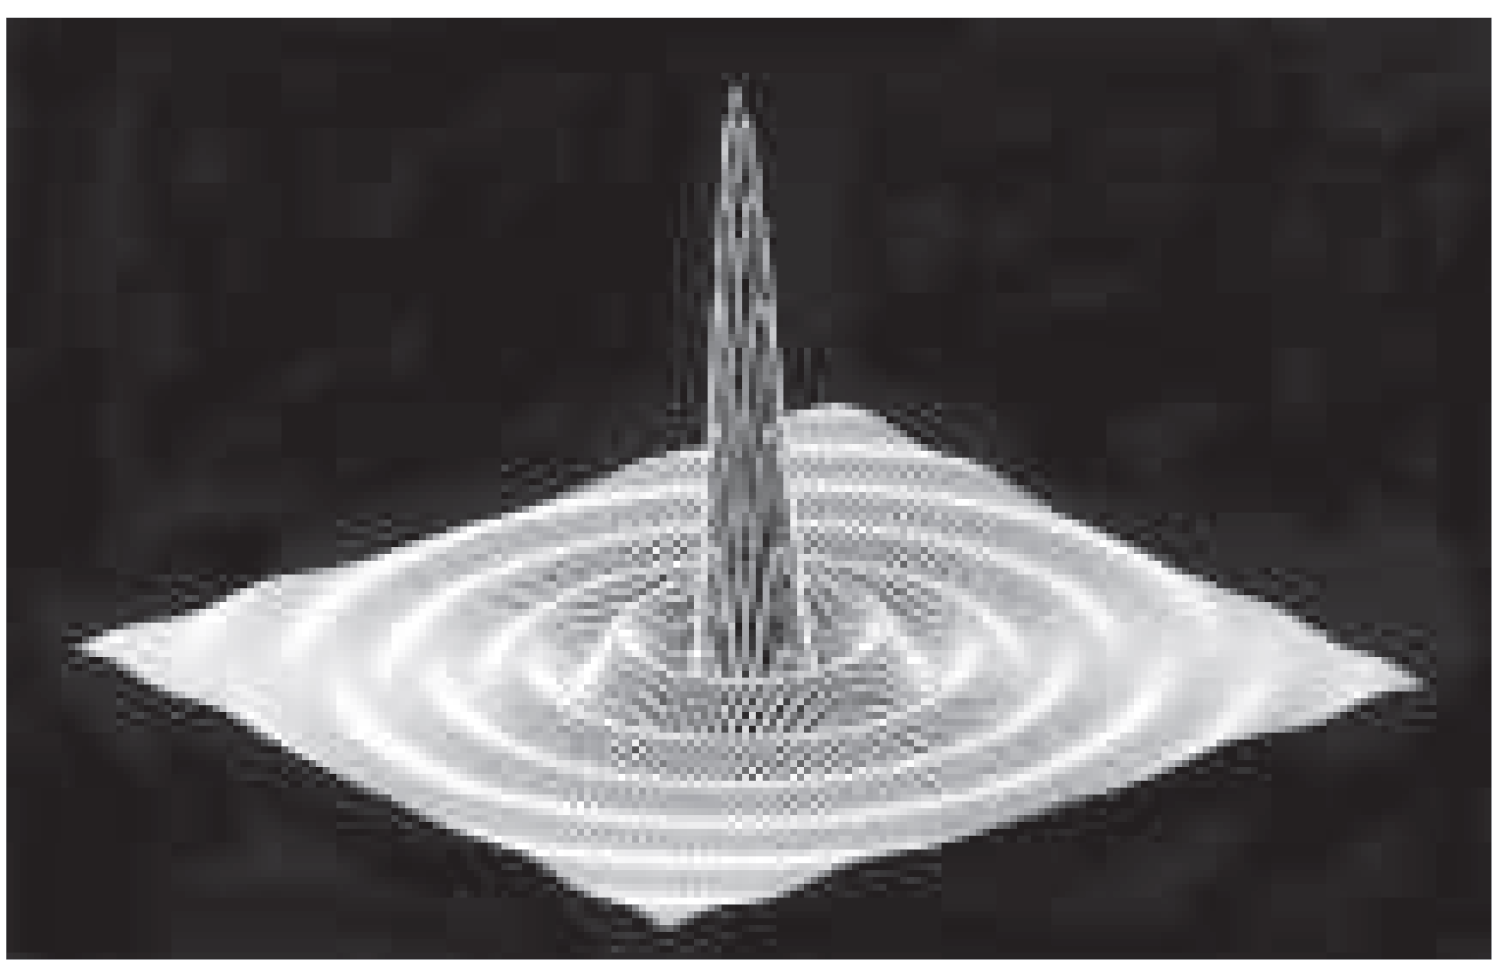
\includegraphics[scale=0.3]{07-Airy.png}
    \caption{función de airy}
    \label{Fig:07.3-01}
\end{figure}


\subsection{Poder de resolución}
Es evidente que la estructura difraccional de la imagen de un punto luminoso axial producido por una lente es la misma que la imagen producida en el foco de una lente cuando esta se ilumina normalmente con una onda plana. De hecho una onda plana es análoga a una esférica procedente del infinito. Por otra parte la \textit{resolución} o discernimiento transversal de dos imágenes en el mismo plano producidas por un sistema óptico de dos fuentes puntuales (incoherentes) verá determinada según el criterio de resolución elegido. 

\subsubsection{Poder de resolución espacial: Rayleigh}

El criterio de resolución de Rayleigh establece que para resolver justamente dos puntos próximos en la imagen, el centro de la mancha de Airy de uno coincide con el primer mínimo de la de otro:

\begin{equation}
    q = 1.22 \frac{\lambda_0 f}{D} \ \Rightarrow \ \Delta \theta_{\min} = \Delta \Phi_{\min} = \frac{q}{f} = 1.22 \frac{\lambda_0}{D}
\end{equation}

\subsubsection{Poder de resolución espacial: Sparrow}

Sparrow propone tomar como límite de resolución una distancia menor, correspondiente a la condición

\begin{equation}
    \ccorchetes{\derivadas{^2 I(r)}{r^2}}_{r<S_p} = 0
\end{equation}
La distribución de intensidad resultante de la superposición de las dos figuras de Airy alcanza un máximo plano cuya anchura coincidirá con la separación entre los picos individuales. 

\section{Redes de difracción ópticas}

\subsection{Difracción de fraunhofer bajo traslaciones de la abertura}

Recordemos el patrón interferencial de una abertura centrada en $x_0=y_0=0$. Consideremos una abertura desplazada un $x_0=x_0'+q_0$ y $y_0=y_0'+p_0$. Cuando iluminamos la abertura desplazada tendremos que:

\begin{equation}
    \psi'(x,y,z) = \Ecal_0 \int \int t_A (x_0',y_0') \psi (x_0',y_0') e^{-ik_0 (\alpha (x_0'+q_0)+\beta(y_0'+p_0))} \D x_0' \D y_0'
\end{equation}
donde sacando de la integral el factor de fase que no depende de las variables de integración, sino del valor de los desplazamientos, observamos que 

\begin{equation}
    \psi ' (x,y,z) = e^{-ik_0 (\alpha q_0 + \beta p_0)} \psi (x,y,z)
\end{equation}
Al desplazar la abertura no cambia el patrón de difracción solo cambia su fase. Iluminando ambas aperturas $A'$ y $A$ (como en la figura \ref{Fig:07.4-01}) tenemos que 

\begin{equation}
    I_{A+A'} = 2 I_0 \ccorchetes{1+\cos (k_0(\alpha q_0 + \beta p_0))}
\end{equation}
En el caso de dos aberturas estrechas de dimensiones $a$ y $b$ con $b\gg a$ que se estudiaron en el capítulo \ref{Chapter:2}, tenemos el interferómetro de Young. 


\begin{figure}[h!]
    \centering
    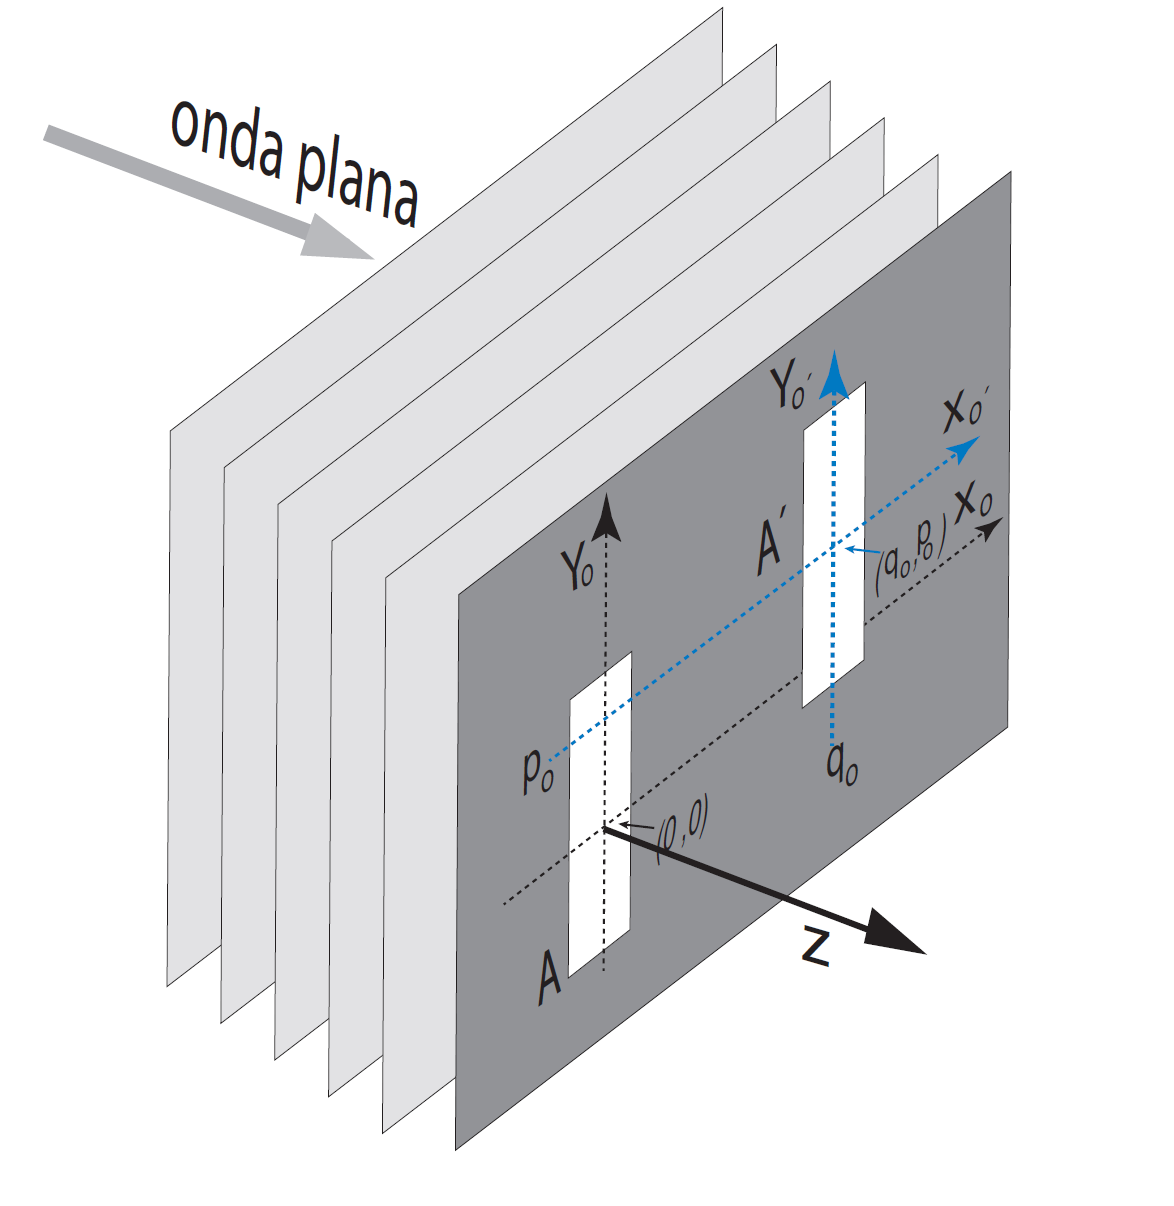
\includegraphics[scale=0.35]{07-Redesdifraccion.png}
    \caption{}
    \label{Fig:07.4-01}
\end{figure}

\subsubsection{La doble rendija}
Los campos difractados por cada rendija son:

\begin{equation}
    \psi_1(x,y,z) = 4 \Ecal_0 ab \sinc \parentesis{\frac{k_0a}{z}x} \quad 
    \psi_2(x,y,z) = 4 \Ecal_0 ab e^{-ik_0 \frac{d}{z}x} \sinc \parentesis{\frac{k_0a}{z}x}
\end{equation}
El patrón de difracción cuando interfieren las amplitudes de ambas rendijas será:

\begin{equation}
I(x,y,z) = I_{00} \sinc^2(k_0ax/z) \ccorchetes{1+\cos\parentesis{k_0 \frac{d}{z}x}}    
\end{equation}

\begin{figure}[h!]
    \centering
    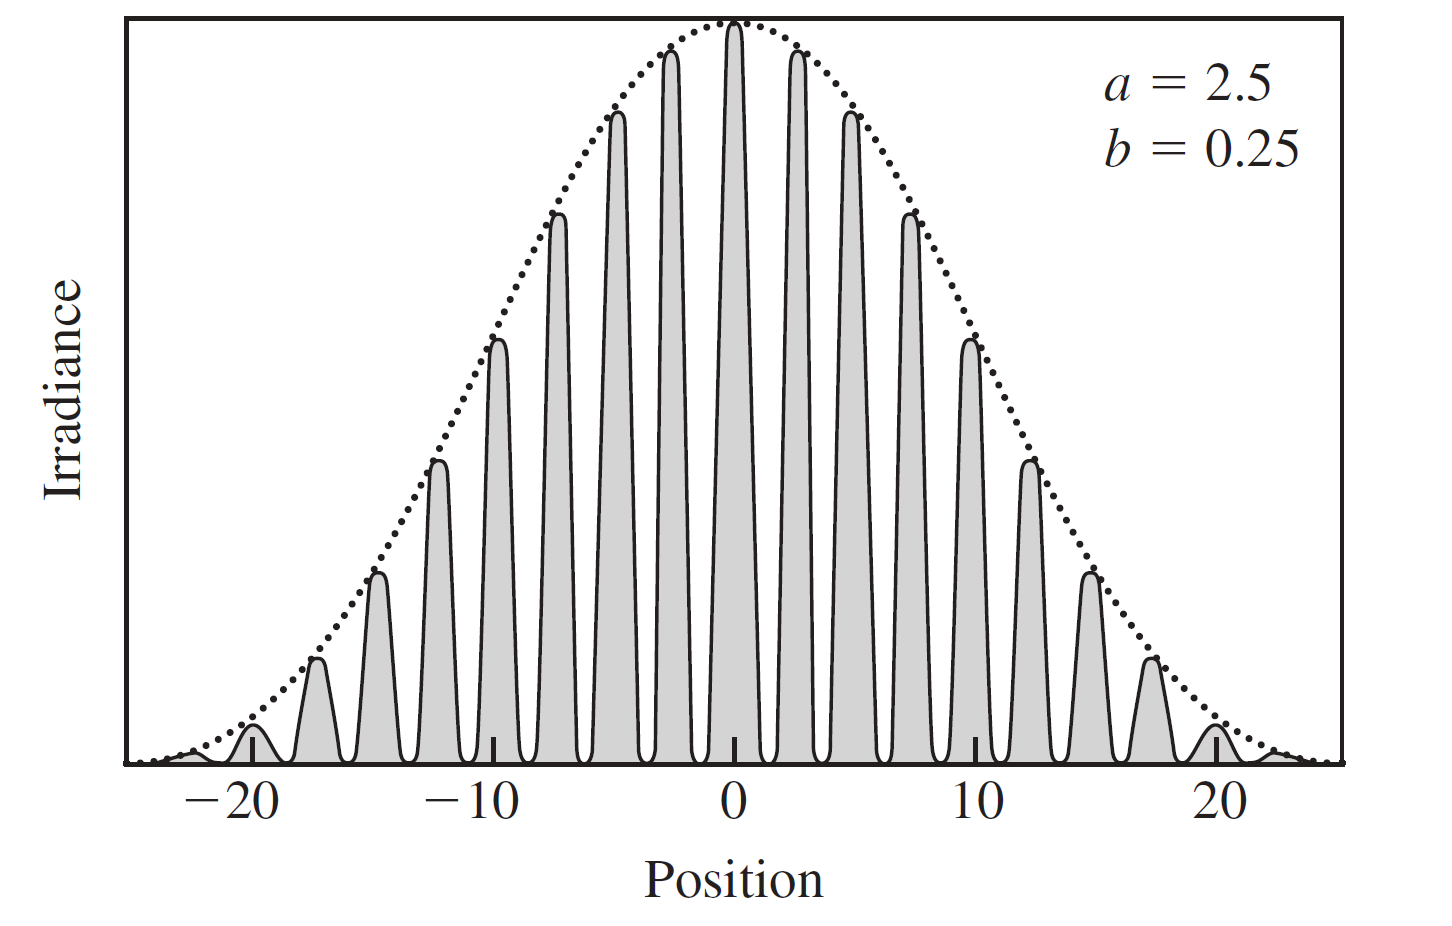
\includegraphics[scale=0.35]{07-Doblerendija.png}
    \caption{}
    \label{Fig:07.4-02}
\end{figure}



\subsubsection{Superposición de $N$ rendijas}

\begin{figure}[h!]
    \centering
    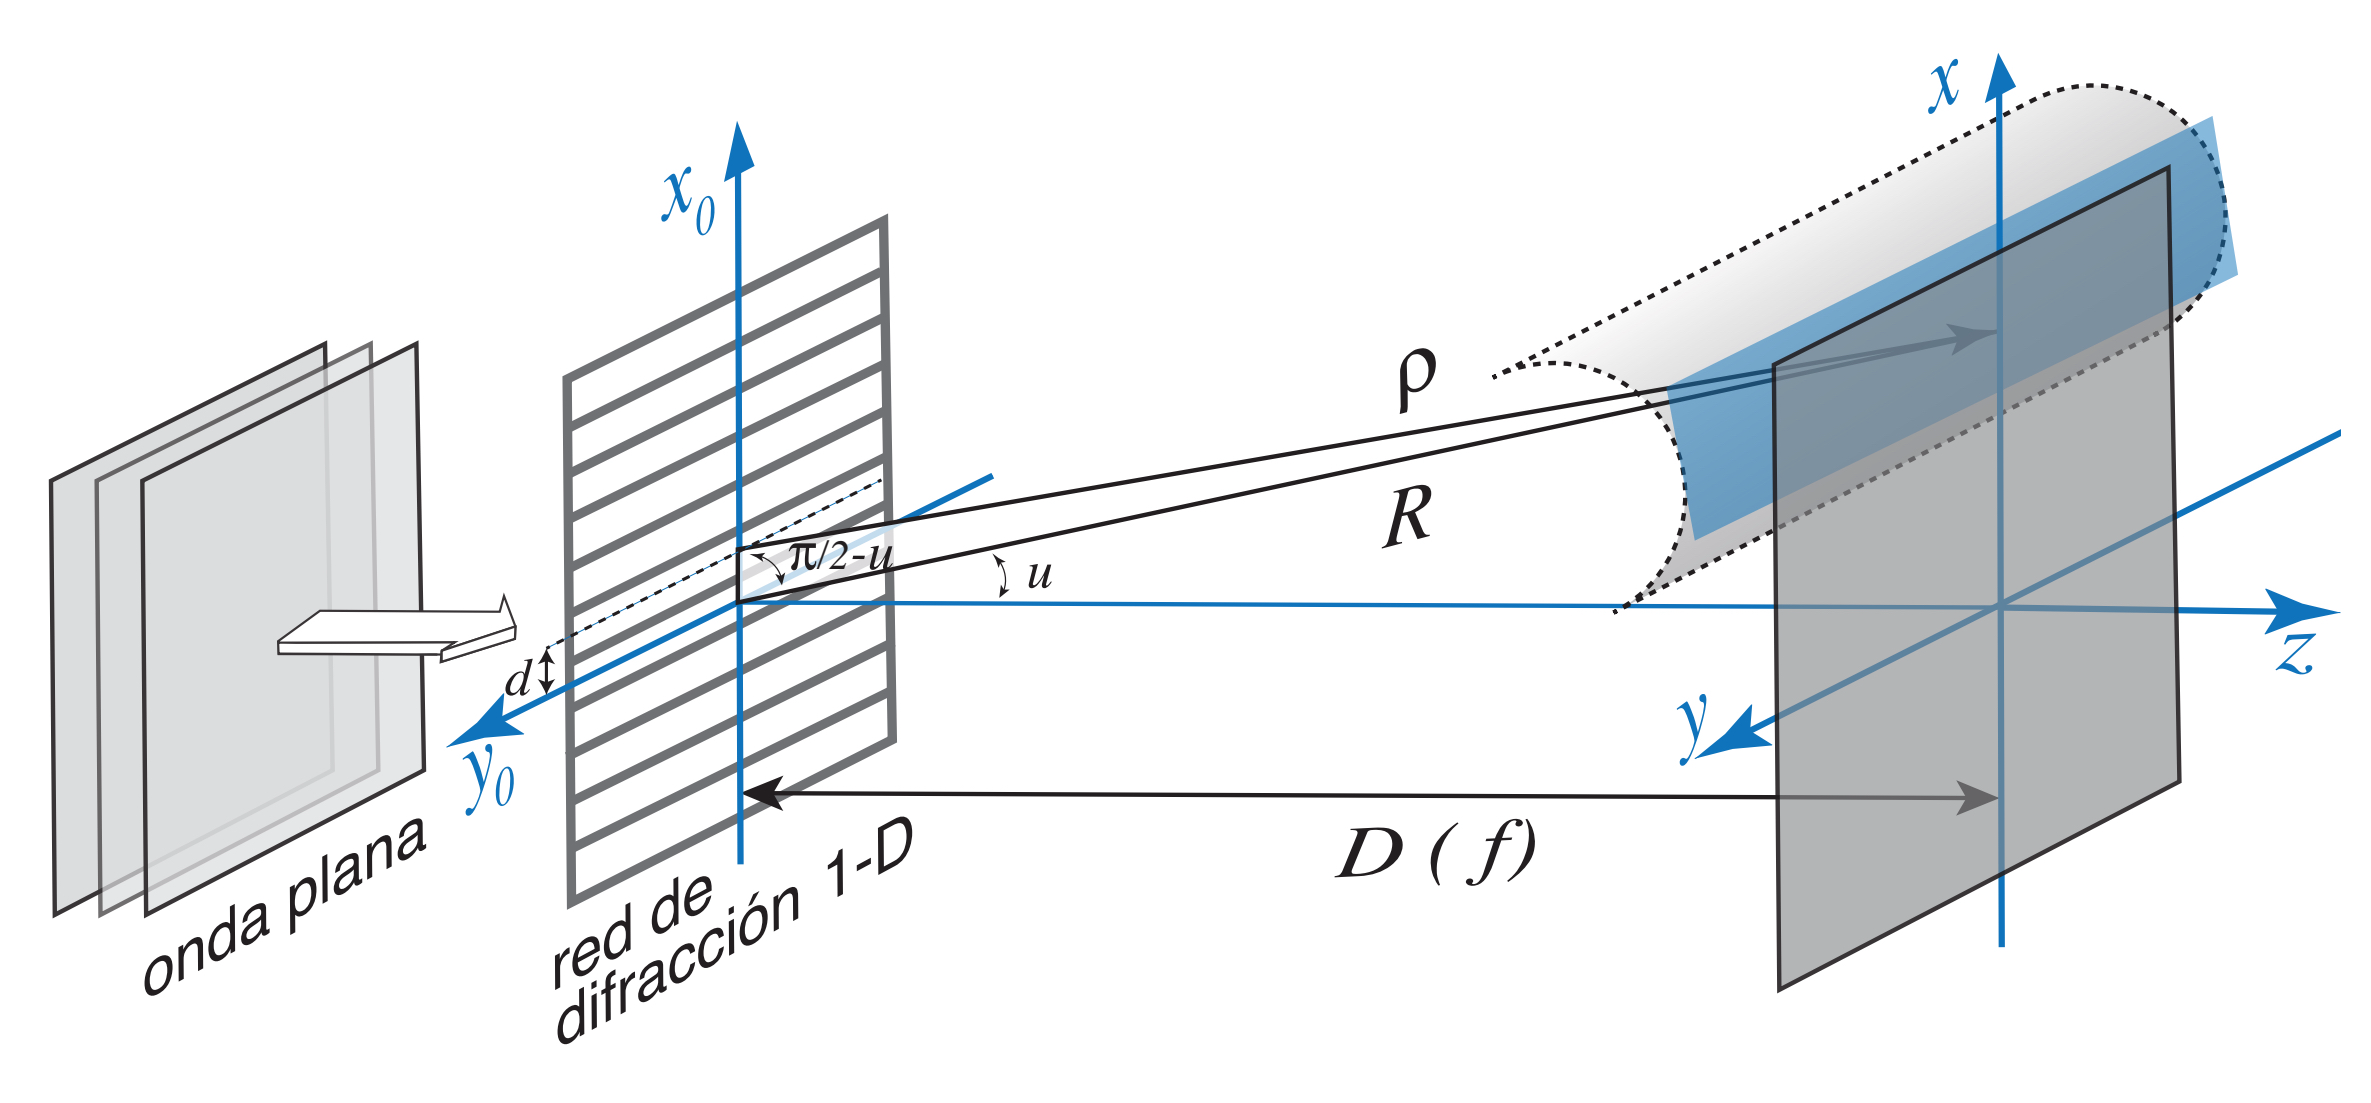
\includegraphics[scale=0.2]{07-Redesdifraccion2.png}
    \caption{}
    \label{Fig:07.4-03}
\end{figure}

Sea la fase en coordenadas cilíndricas $k_0\rho$. Debemos aplicar el teorema del coseno al triángulo que se puede ver en la figura \ref{Fig:07.4-03}. Así tendremos que

\begin{equation}
    \rho \approx R - x_0 \sin (u) 
\end{equation}
donde $R^2=D^2+x^2$. En ese caso tenemos que la amplitud de una rendija, que es una onda cilíndrica, viene dada por 

\begin{equation}
    \psi (x,x_0,u) \approx \frac{1}{R^{1/2}} e^{ik_0 R} e^{-ik_0 x_0 \sin (u)} = \mathcal{A} e^{-ik_0 x_0 \sin (u)}
\end{equation}
donde hemos usado las aproximaciones necesarias. Suponiendo $N$ rendijas con sus correspondientes desfases $\delta$ debido al desplazamiento $d$ en el plano $x_0=0,d,2d\ldots \rightarrow \delta = k_0 \Delta = k_0 d \sin (u)$. La amplitud total debida a las N rendijas será:

\begin{equation}
    \psi  (\delta) = \mathcal{A} \ccorchetes{1+e^{-i\delta}e^{-i2\delta}+\cdots+e^{-i(N-1)\delta}+} = \mathcal{A} \frac{1-e^{-iN\delta}}{1-e^{i\delta}}
\end{equation}
esto es, una progresión de tal modo que la intensidad, salvo el factor $1/R$, viene dada por

\begin{equation}
    I (\delta ) = \sinc(k_0 a x /f) \frac{\sin^2(N\delta  /2)}{\sin^2(\delta/2)}
\end{equation}

\begin{figure}[h!]
    \centering
    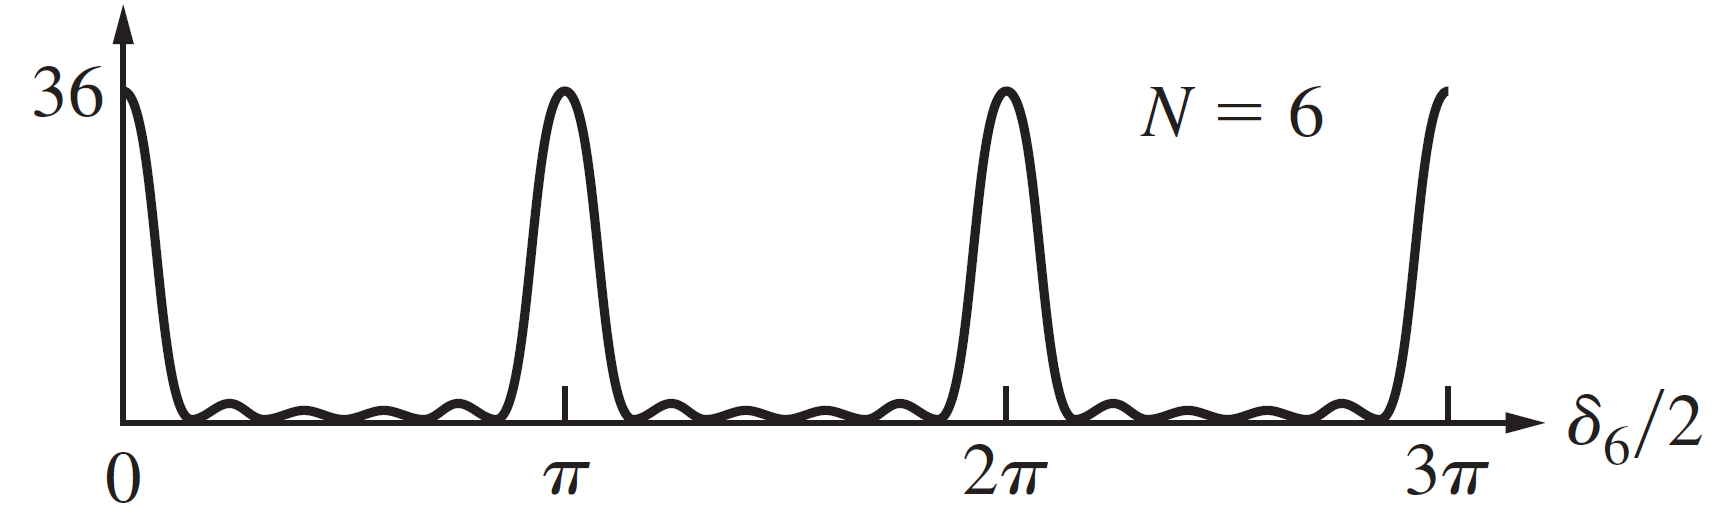
\includegraphics[scale=0.2]{07-Multiplesrendijas.png}
    \caption{}
    \label{Fig:07.4-05}
\end{figure}


\subsection{Propiedades espectrales de las redes}

Para evaluar la semi-anchura del máximo principal calculemos primero la posición del primer mínimo:

\begin{equation}
    \delta_{\min} = \frac{2n \pi}{N} \ \Rightarrow \ \Delta \delta_{1/2} = 2 \pi / N   
\end{equation}

la \textbf{anchura} del máximo principal será entonces

\begin{equation}
    \Delta \delta = 2 \Delta \delta_{1/2}
\end{equation}
La \textbf{anchura angular} $\Delta u_{1/2}$ alrededor de un máximo principal angular $u_m$:

\begin{equation}
    \delta = k_0 d \sin (u_m) \ \Rightarrow \ \Delta \delta = k_0 d \cos (u_m) \Delta u_m
\end{equation}
es decir

\begin{equation}
    \Delta u \approx \frac{\Delta \delta}{k_0 d \cos (u_m)}  \tquad \Delta u \approx \frac{4 \pi}{k_0 d N} \ \mathrm{si} \ u \ll
\end{equation}
considerando la focal de la lente, la anchura lineal será:

\begin{equation}
   \tan (u_m) = \frac{x_m}{f} \Rightarrow \Delta x \approx \frac{f\Delta u_m}{\cos^2(u_m)}  \tquad x_m \approx \frac{4 \pi f}{k_0 d N} \ \mathrm{si} \ u \ll
\end{equation}





\begin{thebibliography}{n}
\bibitem{libro-1} David Griffiths; 
{\it Introduction to Electrodynamics}; Pag 342-344. 


\end{thebibliography}




\end{document}